\documentclass[a4paper,11pt,oneside]{book}

\usepackage[a4paper,left=2.5cm,right=2cm]{geometry}
\usepackage[utf8]{inputenc}%%%Este paquete permite poner acentos directamente%%%
\usepackage[spanish]{babel}
\usepackage{eurosym}
\usepackage[T1]{fontenc}
\usepackage{lmodern}
\usepackage{fancyvrb}
\usepackage{hyperref}
\usepackage{amsmath,amssymb,amsthm,amscd}
\usepackage[nonumberlist, toc]{glossaries}
\usepackage[pdftex]{color,graphicx}
\usepackage{float}
\usepackage{listingsutf8}

\lstset{language=Python, basicstyle=\footnotesize, breaklines=true, extendedchars=true, texcl=true}

\lstset{literate=
  {á}{{\'a}}1 {é}{{\'e}}1 {í}{{\'i}}1 {ó}{{\'o}}1 {ú}{{\'u}}1
  {Á}{{\'A}}1 {É}{{\'E}}1 {Í}{{\'I}}1 {Ó}{{\'O}}1 {Ú}{{\'U}}1
  {à}{{\`a}}1 {è}{{\`e}}1 {ì}{{\`i}}1 {ò}{{\`o}}1 {ù}{{\`u}}1
  {À}{{\`A}}1 {È}{{\'E}}1 {Ì}{{\`I}}1 {Ò}{{\`O}}1 {Ù}{{\`U}}1
  {ä}{{\"a}}1 {ë}{{\"e}}1 {ï}{{\"i}}1 {ö}{{\"o}}1 {ü}{{\"u}}1
  {Ä}{{\"A}}1 {Ë}{{\"E}}1 {Ï}{{\"I}}1 {Ö}{{\"O}}1 {Ü}{{\"U}}1
  {â}{{\^a}}1 {ê}{{\^e}}1 {î}{{\^i}}1 {ô}{{\^o}}1 {û}{{\^u}}1
  {Â}{{\^A}}1 {Ê}{{\^E}}1 {Î}{{\^I}}1 {Ô}{{\^O}}1 {Û}{{\^U}}1
  {œ}{{\oe}}1 {Œ}{{\OE}}1 {æ}{{\ae}}1 {Æ}{{\AE}}1 {ß}{{\ss}}1
  {ű}{{\H{u}}}1 {Ű}{{\H{U}}}1 {ő}{{\H{o}}}1 {Ő}{{\H{O}}}1
  {ç}{{\c c}}1 {Ç}{{\c C}}1 {ø}{{\o}}1 {å}{{\r a}}1 {Å}{{\r A}}1
  {€}{{\EUR}}1 {£}{{\pounds}}1
}



\definecolor{rojo}{rgb}{1,0,0}
\definecolor{negro}{rgb}{0,0,0}

\parskip=5mm

\newglossaryentry{Guitar Hero}{name=Guitar Hero, description={Juego lanzado en 2005, por Harmonix que se basa con el controlador en forma de guitarra simula a una guitarra verdadera}}

\newglossaryentry{Rock Band}{name=Rock Band, description={Juego lanzado en 2007, que se basa en simular una banda de rock, con sus diferentes partes vocales, guitarra y bajo, batería y piano}}

\newglossaryentry{Pads}{name=Pads, description={Parte de una batería-MIDI donde se ha de golpear para que imite el sonido de ese instrumento, normalmente cada pad solo emite una nota, variando su potencia dependiendo del golpe, la excepción suele ser el charles que tiene posición abierto y cerrado, en las baterías profesionales hay pads que tienen varias zonas de golpeo y emiten un sonido dependiendo de la zona y la potencia}}

\newglossaryentry{Lanes}{name=Lanes, description={Columnas donde van los chips visuales del juego musical}}

\newglossaryentry{Chips}{name=Chips, description={Nota visual que va bajando por los lanes para indicarnos cuando se ha de tocar}}


\makeindex
\makenoidxglossaries


\begin{document}
 
\title{Reproductor de canciones DTXMANIA para entornos libres}
\author{Guillermo Eduardo Cabezas Castillo}
\date{\today}

\maketitle 

\tableofcontents
\listoffigures
\chapter*{Agradecimientos}
\begin{flushright}
\textit{Dedicado a \\
mi familia}
\end{flushright}

\chapter{Introducción}

	 El objetivo de este proyecto es un reproductor de canciones DTXMANIA, en entornos de código abierto. Para ello se tendrá que implementar la idea de como es este formato, y que es necesario hacer para poder reproducirlo con algunos de sus añadidos.


\par
  Como primera toma de contacto se puede decir que el formato DTXMANIA, es un formato musical, especializado en baterías.

\section{El proyecto DTXMANIA en el contexto actual}
  
  El origen del formato DTXMANIA proviene de una serie de juegos musicales desarrollados en Japón. Cuando los usuarios de dichos juegos que tenían conocimientos prácticos del uso de instrumentos de percusión (en concreto baterías) los probaron, se dieron cuenta de que con una serie de modificaciones adicionales dichos juegos podían ser un apoyo eficiente para mejorar su técnica habitual. De aquí surge la idea de desarrollo de este proyecto en el que se propone y se lleva a cabo un entorno basado en software libre para posibilitar el uso de dicha práctica.
  
  Debido al auge que han tenido este tipo de juegos a partir del famoso \gls{Guitar Hero}, con la finalidad de mostrar el amplio abanico de juegos e ideas existentes en el mercado, se hace necesario exponer un conjunto representativo de los principales juegos de tipo musical que disponen de un componente físico para simular instrumentos.
  
  En consecuencia a la gran diversidad de entornos y sistemas existentes también se hace necesario efectuar un pequeño repaso a los formatos musicales digitales que dan soporte a dichos desarrollos ya que van a estar altamente integrados en este proyecto.
  
\subsection{Historia de los principales juegos musicales}
	Cuando se piensa en un juego/simulador principal lo que primero puede venir a la mente, por ser lo más conocido es el caso del \Gls{Guitar Hero}, aunque es el más conocido también se tiene que hacer un repaso a otros juegos de corte musical para poder entender la evolución de este tipo de juegos y más concretamente los que tienen como instrumento principal la batería ya que sera uno de los principales objetivos del proyecto.

\subsubsection{Guitar Hero}
\gls{Guitar Hero} es una popular franquicia de videojuegos musicales.

La serie \gls{Guitar Hero} es conocida por el uso de un dispositivo con forma de guitarra que se utiliza como control de juego para simular y hacer música con ella, representando notas de colores en la pantalla que corresponde a cada uno de los botones del controlador. Los juegos de la serie permiten tanto partidas individuales como multijugador, pudiendo estas últimas ser cooperativas o competitivas. La serie ha utilizado una amplia gama de canciones de rock de diversas épocas, tanto licenciadas como independientes, hechas desde los años 60 hasta el presente, muchas de ellas son de bandas muy exitosas.

La serie ha vendido alrededor de 15 millones de juegos, ganando aproximadamente 1000 millones de dólares.



\gls{Guitar Hero} es un juego inusual debido a que viene con un control que recrea a una ``Gibson les Paul'' en lugar de los controles comunes. Jugar con el controlador en forma de guitarra simula a una guitarra verdadera, a excepción de los ``Botones Traste'' y la ``Barra de Sonido'' en lugar de los Trastes y las seis cuerdas. El desarrollo de Guitar Hero fue inspirado en el juego Guitar Freaks de Konami, que en esos tiempos no era muy popular en Estados Unidos.

\begin{figure}[H]
% Centramos la figura
\begin{center}
% Incluimos el gráfico y definimos el ancho y alto
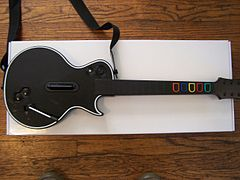
\includegraphics[scale=2.0]{Imagenes/Guitar_Hero_3_controller.jpg}
% Ponemos Leyenda al gráfico
\caption{Controlador del Guitar Hero}
\label{Controlador del Guitar Hero}
\end{center}
\end{figure}


Su control básicamente son unos \gls{Chips}  que van bajando por la pantalla y se tiene que sincronizar el pulsar el botón asociado de la guitarra simulada cuando llegan a la parte más baja. Estos chips están sincronizados con la canción.


\begin{figure}[H]
% Centramos la figura
\begin{center}
% Incluimos el gráfico y definimos el ancho y alto
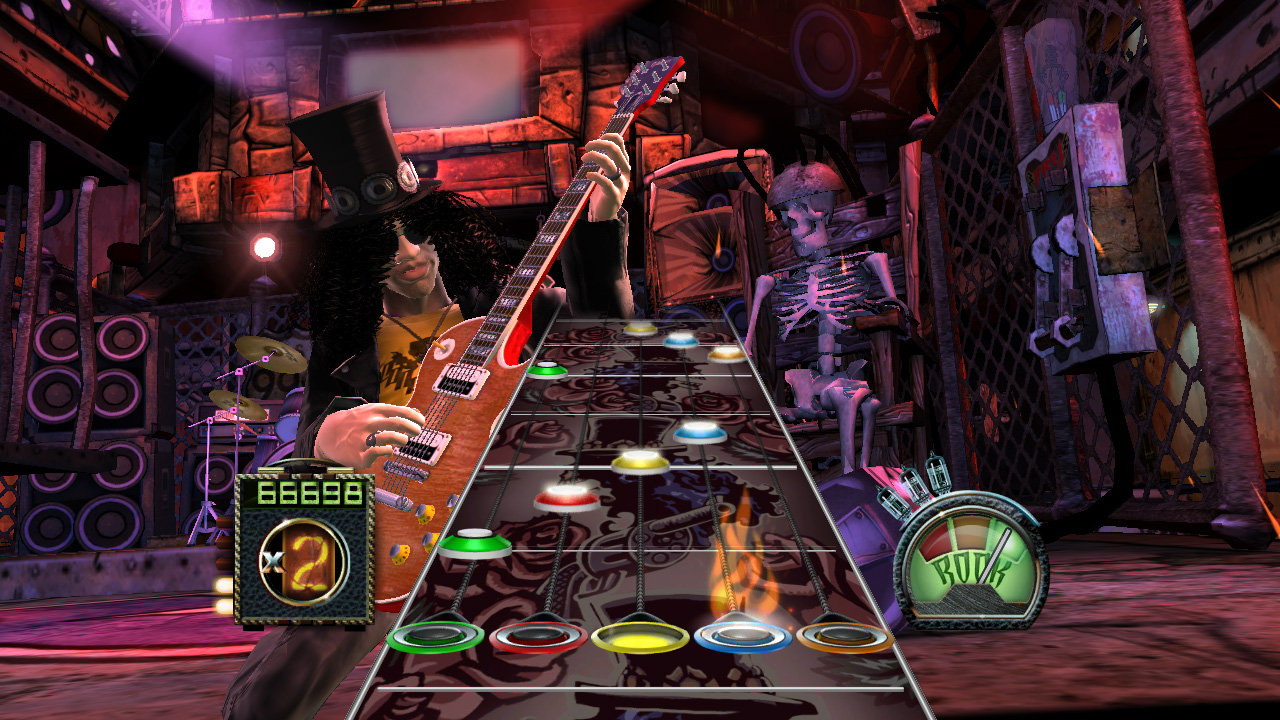
\includegraphics[scale=0.3]{Imagenes/guitar-hero-3.jpg}
% Ponemos Leyenda al gráfico
\caption{Interfaz del Guitar Hero}
\label{Interfaz del Guitar Hero}
\end{center}
\end{figure}

Comentar que hay una barra de vida y esta baja o sube según vamos dando a las notas más correctamente o menos. Si la vida bajara mucho se para la canción y se vuelve al menú principal.


\subsubsection{Rock Band}

Los productores del juego \gls{Guitar Hero} después de lanzar varias versiones de éste, constataron que el empuje inicial de la dinámica de juego se estaba quedando obsoleto y que si deseaban continuar debían de aportar nuevas ideas al producto. Es entonces cuando deciden lanzar al mercado el \gls{Rock Band}.

\gls{Rock Band} es una serie de videojuegos de música en los cuales permite que hasta cuatro jugadores puedan jugar a tocar algunas de las canciones más populares de música Rock, jugando con los instrumentos de la empresa(o también con los instrumentos de \gls{Guitar Hero}). Los jugadores pueden jugar con una guitarra, un bajo, una batería y cantando con un micrófono, además de el teclado (desde el Rock Band 3)

Exceptuando el control de micrófono, la idea básica continua siendo la misma, simular en mejor o peor medida los instrumentos antes citados, con el sistema ya creado en el \gls{Guitar Hero}.


La primera batería que salio a la venta para el \gls{Rock Band} en principio contaba solamente con cuatro \gls{Pads} y un pedal.

\begin{figure}[H]
% Centramos la figura
\begin{center}
% Incluimos el gráfico y definimos el ancho y alto
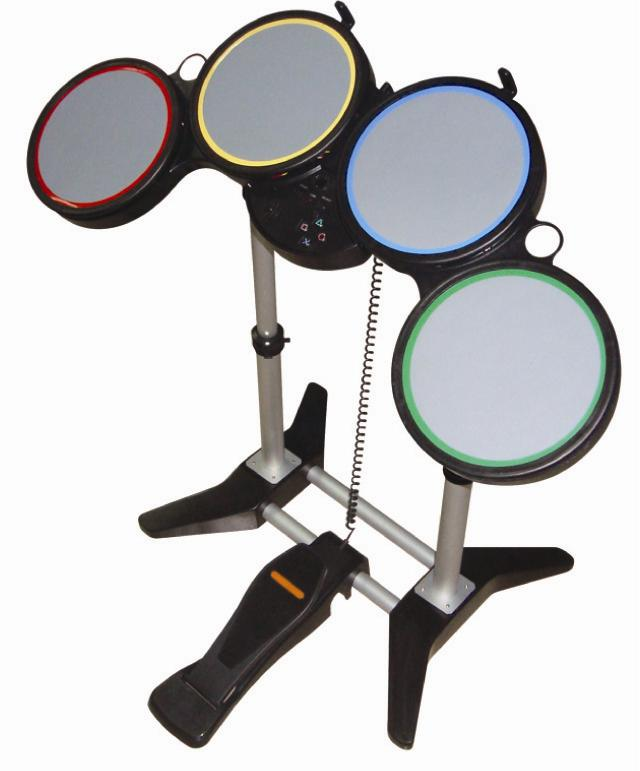
\includegraphics[scale=0.3]{Imagenes/Drum-Controller-for-Rock-Band.jpg}
% Ponemos Leyenda al grafico
\caption{Batería de Rock Band}
\label{Batería de Rock Band}
\end{center}
\end{figure}

Más adelante con el juego Rock Band Pro, ya salio la posibilidad de una batería con siete \gls{Pads} y un pedal, evidentemente con la batería avanzada se podía jugar con las canciones de la batería básica.

\begin{figure}[H]
% Centramos la figura
\begin{center}
% Incluimos el gráfico y definimos el ancho y alto
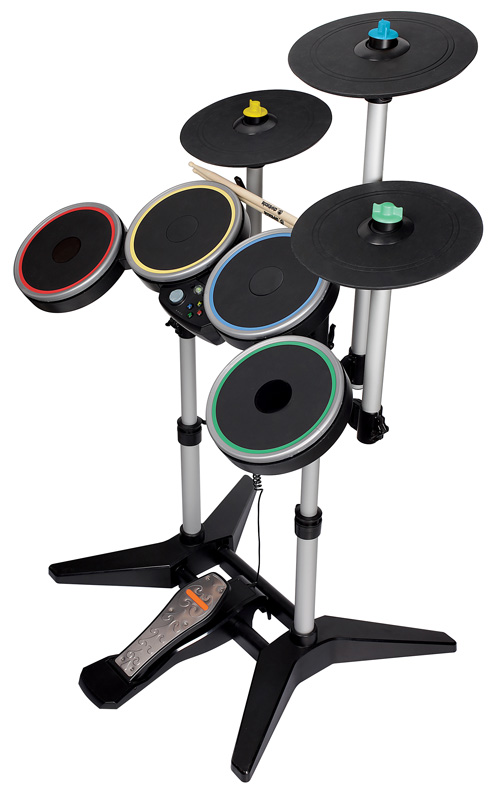
\includegraphics[scale=0.2]{Imagenes/rb3-drums.jpg}
% Ponemos Leyenda al grafico
\caption{Batería de Rock Band Pro}
\label{Batería de Rock Band Pro}
\end{center}
\end{figure}

Uno de los problemas que tuvo la gente al encontrarse con estas canciones con un nuevo formato, es que la compañía solamente dio la posibilidad de actualizar las canciones antiguas al nuevo formato pagando.


\subsubsection{Frets on fire}
Debido al auge de estos juegos musicales no se tardo en sacar una versión libre de estos, el más famoso de ellos fue el Frets on fire, que copiaba el juego \gls{Guitar Hero}.
De modo que el jugador simula el acto de tocar una guitarra. Las notas aparecen en la pantalla sincronizadas con la canción, y son tocadas manteniendo presionadas las teclas correctas y marcándolas pulsando Enter en el momento preciso. El punteo en las notas correctas incrementa el coeficiente por el que se multiplican los puntos ganados al tocar (x2, x3 y hasta x4), pero una sola nota incorrecta hace que este coeficiente vuelva a x1. Si bien no hay ningún objetivo establecido para las canciones, la puntuación obtenida puede ser comparada con la del resto de jugadores en la web oficial.

El carácter más distintivo del juego es la forma de controlarlo: el teclado se coge con ambas manos como si de una guitarra se tratase, con la mano izquierda en los botones F1-F5 y la derecha en el botón Enter. Debido que algunos teclados no reconocen la pulsación simultánea de algunas de estas teclas, el juego permite cambiarlas para evitar este problema.

Su fecha de salida fue el 3 de agosto de 2006. Un detalle muy importante es que de inicio ya incorporaba el poder agregar ``mods'' para maximizar su funcionalidad y modificar su apariencia física según los gustos del jugador.

\subsubsection{FoFiX}
Un mod muy famoso del Frets on Fire fue el FoFix fue una versión libre del \gls{Rock Band}.

Estos juegos al ser libres todo su código se puede mirar y modificar. Aunque mayoritariamente fueron detrás de sus originales en cuanto a las modificaciones que se programaban. Si el \gls{Guitar Hero} insertaba un modo donde las canciones eran más difíciles al cabo de un tiempo en el Frets on fire se programaba un mod para ello. 
Un punto a favor de estos juegos es que si se tenía el juego original se podía copiar las canciones de estos juegos y además disponer de las propias que la comunidad creaba para ellos. Evitando de esta manera tener solo una única tienda donde estaba todo el control sobre las canciones que se creaban y sus precios.

\subsubsection{Dance Dance Revolution}
Dance Dance Revolution es la serie pionera del género de simuladores de baile en los vídeo juegos. Los jugadores se colocan sobre una ``plataforma de baile'', también llamada ``pista'' y presionan con los pies las flechas dispuestas en forma de cruz sobre esta pista, siguiendo el ritmo de la música y el patrón visual que aparece en la pantalla. De acuerdo a la sincronización que los jugadores muestren con el ritmo y lo bien que sigan el patrón de flechas, se les otorgara una puntuación (que varía de acuerdo a la versión del juego). Su primer lanzamiento, en forma de árcade, fue realizado en Japón en 1998. Desde su creación han sido producidas múltiples variaciones, incluyendo algunas para uso casero. Es clasificado como un juego Bemani (Bemani es una abreviación japonesa de la palabra Beat Mania, el nombre del primer juego musical de Konami), cuyo creador es Yoshihiko Ota, que también participó en otras series como ``pop'n music''.

En la composición de canciones para el juego participan varios artistas, incluyendo los que aparecen en la serie de discos Dance Mania, otros de Konami, como Yasuhiro Taguchi, principal compositor musical para esta serie de juegos desde DDR X y pocos, como Naoki Maeda, fundador de la serie, que se retiraron de Konami. Algunos artistas han dado letras de sus canciones como es el caso de Aerosmith que donó la canción ``I Don't Want to Miss a Thing'' para el Dance Dance Revolution Extra Mix que también está disponible en versión para PlayStation.


Durante un juego normal, 4 flechas direccionales (u 8 en Double) permanecen estáticas en la parte superior de la pantalla. Otras flechas se desplazan desde la parte inferior de la pantalla hasta las flechas estáticas en la parte superior (se cambia de posición en caso de que el jugador opte por Reversa). Un jugador debe bailar con la canción, pisando la superficie correspondiente a las flechas marcadas en la pantalla en una plataforma de baile de metal y acrílico. En algunas ocasiones dos o más flechas deben ser pulsadas al mismo tiempo, lo que obliga al jugador a saltar para pulsar 2 flechas a la vez o agacharse para pulsarlas con las manos o rodillas, en caso de 3 o 4 flechas consecutivas, estas últimas aparecen en los edits. De esta manera, el juego invita al jugador a bailar según la coreografía pre-establecida para cada canción. Por otro lado se encuentran las Freeze Arrow (implementadas desde DDRMAX) que aparecen flechas en las que hay que mantener presionado el botón correspondiente durante el tiempo establecido. A veces, ciertas canciones tienen pausas de tiempo, sobre todo, antes de la flecha o al empezar el frezze arrow, el jugador debe estar más atento a la secuencia. En algunas ocasiones dos o más Frezze Arrows deben ser pulsadas y mantenidas al mismo tiempo, ya que levantando el pie durante el Frezze Arrow cuenta como una flecha perdida. Y finalmente, las Shock Arrows (implementadas desde DDR X) que solo aparecen en unas determinadas canciones, generalmente en Challenge, y consisten en que aparecen las 4 u 8 flechas al mismo tiempo, en un color metalizado y con unos relámpagos por dentro. La misión del jugador es esquivarlas, ya que de pulsarlas, cuenta como flecha perdida, frena el combo y desaparece las flechas por una fracción de segundo. Este tipo de paso recuerda y mucho a las populares Minas de la serie de juegos musicales ``In the Groove'', de la cual Konami tiene los derechos tras su juicio con Roxor Games. Si se falla repetidamente las flechas (o pisando una Shock Arrow), la barra de vida se vé drásticamente reducida y se puede llegar a fallar la canción.

\begin{figure}[H]
% Centramos la figura
\begin{center}
% Incluimos el gráfico y definimos el ancho y alto
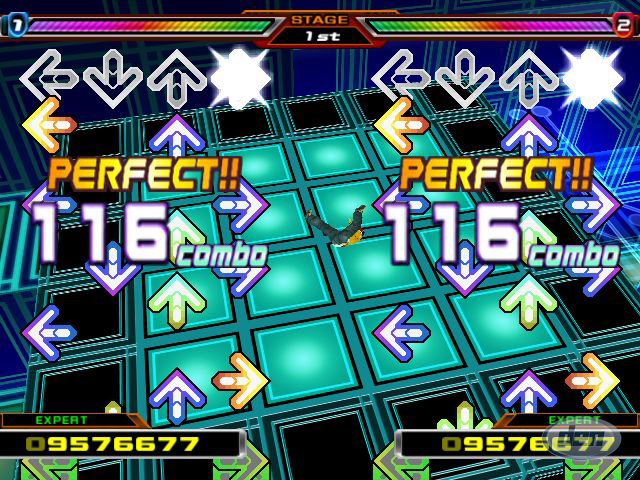
\includegraphics[scale=0.3]{Imagenes/DanceDanceScreen1.jpeg}
% Ponemos Leyenda al gráfico
\caption{Interfaz del DDR}
\label{Interfaz del DDR}
\end{center}
\end{figure}


Dependiendo del tiempo en cada paso, el paso se marca como ``Marvelous'', ``Perfect'', ``Great'', ``Good'', ``Almost'' o ``Miss'' En la parte superior de la pantalla hay una barra de vida, y empieza a la mitad al comienzo de la canción. Los pasos Great o más incrementan la barra de vida hasta que se llena. Mientras que los pasos ``Almost'' y ``Miss'' la disminuyen. Los pasos ``Good'' no tienen efecto positivo o negativo. Si a un jugador reduce su barra de vida totalmente por fallar muchas veces, falla la canción y, solo en Versus, cuando los dos jugadores fallan, o si uno de los dos logra llegar al final de una canción.
 El jugador recibe una puntuación final que puede ir de una ``AAA+'' a una ``E'' (donde ``AAA+'' la mejor calificación obtenida, ``D'' la peor y ``E'' cuando falla la canción), basado en la cantidad de pasos correctos que haya realizado, en la sincronía con el juego y el conteo de calorías quemadas (vista en la evaluación desde Supernova2 y en versiones caseras), y cuando ambos ven una ``E'' o si ha terminado todas las canciones, se termina el juego. Normalmente, si falla la canción en curso, aparece ``FAILED'' en rojo antes de la evaluación, lo mismo ocurre si termina la canción con la palabra ``CLEARED'' en verde.

En una canción, existen factores que determinan su dificultad de baile, los cuales están marcados en pies, desde 4thMIX, los beats por minuto (BPM) y desde el DDRMAX, el Groove radar (desactivado al jugar en modo Happy en X2 y X3). Originalmente, las canciones usaban fondos con gráficos o videos aleatorios, pero desde DDR Supernova, fueron remplazados por videos exclusivos o escenarios, ya que antes no sabían que canción se estaba jugando y desde DDR Supernova 2 apareció el visor de canciones en vez de fondos. Ciertas canciones con video desde DDR X2 aparecen en pantallas del escenario.

\subsubsection{Stepmania}

Stepmania es un video juego de baile y ritmo, entra en la categoría de simulación inspirado en Dance Dance Revolution. Es un software libre y totalmente gratuito, disponible para sistemas como Linux, Windows o Mac OS X, como también su código fuente es utilizado para ``In The Groove'' y ``Pump It Up Pro''.

Es idéntico a Dance Dance Revolution con la diferencia de que el usuario puede interactuar libremente con el programa, pudiendo soportar las canciones de DDR PC e incorporar canciones a su gusto, caratulas, estilos visuales, etc. Las tres primeras versiones usaban la interfaz de DDRMAX. Desarrolladores crearon SM4 en sus dos versiones. La versión CVS estaba basado en la construcción del 2006, llamándose Stepmania 3.95. Chris Danford, creador de Stepmania, bifurcó la otra versión CVS y lo llamó SM 4 Beta. Después del anuncio del 4 beta, varias versiones CVS y SVN no oficiales fueron creadas por la comunidad de Stepmania como una versión 5.

Es totalmente accesible y se puede modificar al gusto de la persona pero siempre manteniendo el estilo clásico de su núcleo.

\subsubsection{Drum Mania}
Drum Mania es un juego musical producido por Bemani, la división musical de Konami.

La fecha de salida de Drum Mania fue en 1999 como un juego arcade, después se porto a la PlayStation 2 en Japon en el año 2000 como un título de salida. Siguientes versiones del juego han salido aproximadamente una al año.

El juego puede ser enlazado con su versión de guitarra Guitar Freaks, permitiendo el juego cooperativo, versiones anteriores también se podían enlazar con Keyboard Mania. Desde el 7th mix hacia adelante, se pudo conectar al sistema de Konami e-Amusement para el juego competitivo on-line.

Drum Mania simula el hecho de tocar una batería real. Se juega usando un controlador que imita a una batería. Seis \gls{Lanes} colocadas de derecha a izquierda como el hi-hat, caja , tom alto , tom de piso , platillos y además un pedal para simular el bombo. Durante el juego, el jugador tiene que tocar los \gls{Pads} y el pedal en sincronía con los \gls{Chips} que van cayendo verticalmente desde arriba, y en sincronía con la música.

\begin{figure}[H]
% Centramos la figura
\begin{center}
% Incluimos el gráfico y definimos el ancho y alto
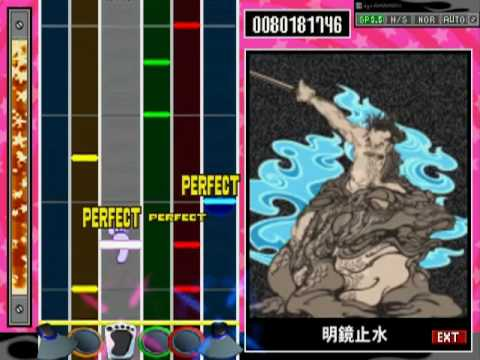
\includegraphics[scale=0.3]{Imagenes/Drum_Mania_interface.jpeg}
% Ponemos Leyenda al gráfico
\caption{Interfaz del Drum Mania}
\label{Interfaz del Drum Mania}
\end{center}
\end{figure}

La exactitud del jugador es juzgada en cada nota, y aunque el sistema de medir esta exactitud se ha cambiado a través de las versiones, actualmente el sistema emplea Perfect, Great, Good, Poor y Miss para evaluar el sincronismo de cada nota. Las categorías de Poor y Miss vaciaran el ``Excite Gauge'' del jugador mientras que mantener el sincronismo lo aumentara. Si el ``Excite Gauge'' se vaciá completamente el juego acaba. Los jugadores podrán jugar de tres a cinco canciones dependiendo de la configuración y según sus puntuaciones podrán jugar dos canciones adicionales. Cuando se completa una canción a los jugadores se les otorga una puntuación que va desde E hasta A, también incluyendo S y SS dependiendo de lo bien que hayan tocado la canción y la configuración de la puntuación en esa versión.

Drum Mania usa una batería electrónica modificada de Yamaha de la gama DTXPRESS. Esta batería es usada para navegar por los menús y pantallas de selección, también se puede navegar mediante los botones Select y Start en los laterales de la máquina. 


\begin{figure}[H]
% Centramos la figura
\begin{center}
% Incluimos el gráfico y definimos el ancho y alto
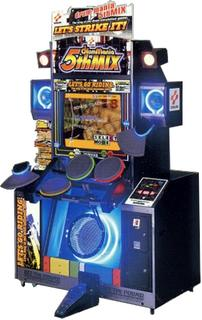
\includegraphics[scale=0.5]{Imagenes/cabinet-drummania.jpg}
% Ponemos Leyenda al gráfico
\caption{Mueble arcade del Drum Mania}
\label{Mueble arcade del Drum Mania}
\end{center}
\end{figure}

\subsubsection{Drum Mania XG / Gitadora}

En el año 2010 la serie se cambio de nombre a Drum Mania XG, aquí se introdujo el cambio en los controles de añadir un tom de suelo, un cymbal izquierdo y un pedal izquierdo a la maquina original, y para que hubiera más desarrollo en este nuevo juego se paro el desarrollo en la saga Drum Mania.

Más adelante en el año 2012 se cambio el nombre de Drum ManiaXG a Gitadora, dejando los controles iguales, limpiando mucho la interfaz del Drum ManiaXG y modificando los modos de conexión a Internet, fueron los principales cambios.


\begin{figure}[H]
% Centramos la figura
\begin{center}
% Incluimos el gráfico y definimos el ancho y alto
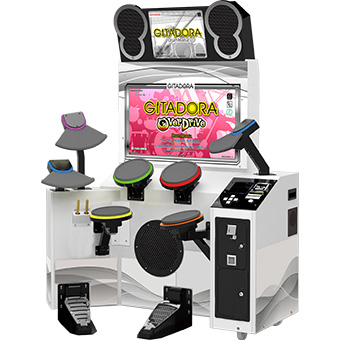
\includegraphics[scale=0.5]{Imagenes/cabinet-gitadora.jpg}
% Ponemos Leyenda al gráfico
\caption{Mueble arcade del Gitadora}
\label{Mueble arcade del Gitadora}
\end{center}
\end{figure}


\subsubsection{DTXMania}
El DTXMania es un juego musical basado en el Drum Mania, su programador lo llego a liberar en el año 2000 bajo la licencia MIT. Su idea original era coger el Drum Mania y poder ejecutarlo en un ordenador, al principio pensado para las baterías electrónicas Yamaha y poco a poco lo fue modificando para poder conectar cualquier batería electrónica MIDI, que al final se ha convertido en su principal objetivo.

Ya desde el inicio se fue separando del proyecto Drum Mania para acercarse más a un simulador real, antes que a un juego.

Fue el primero en implementar el hihat abierto y cerrado, de esta manera y si la batería MIDI tenia esta posibilidad tener que usar el pedal izquierdo, para tocar el hihat tal y como se tendría que hacer en una batería real. Siempre se dejaba el escoger como funcionaban estas opciones que programaba por si tu batería no era tan potente o por si querías acercarte más a un juego antes que a un simulador.

Se expone la manera de puntuar clásica:

     (Porcentaje de notas en Perfect x .85) + (Porcentaje de notas en Great x .35) + (Porcentaje de Max Combo x .15)

Basado en este ratio, se asignan las siguientes puntuaciones:

\begin{itemize}
  \item SS = 95.00+ 
  \item S = 80.00 - 94.99
  \item A = 73.00 - 79.99
  \item B = 63.00 - 72.99
  \item C = 53.00 - 62.99
  \item D = 45.00 - 52.99 
  \item E = 0 - 44.99 
\end{itemize}
    

Un detalle que muestra uno de los motivos que gusto a la gente que toca la batería es el siguiente, se puede tocar todas las notas de una canción y sí se ha cometido algún fallo de sincronismo no tener la canción al 100\%.

Muchos baterías vieron en este programa una gran ayuda para sus sesiones de practica gracias principalmente a dos puntos.

\begin{itemize}
\item   1. Poder detallar a que nivel querían el sincronismo.
\item   2. Con la inclusión de poder tocar con la batería electrónica podían entrenar ritmos tal y como se han de tocar en la batería acústica.
\end{itemize}

Poco a poco se fue haciendo una gran comunidad que creaba canciones para el DTXMania y aportaban ideas para cada convertirlo en una ayuda para sus sesiones de entrenamiento.


\subsubsection{DTXManiaHD}
Cuando salio el Drum Mania XG en el año 2010, el programador de DTXMania añadió los cambios que se habían realizado para poder importar las canciones del Drum Mania XG al DTXManiaHD, se hizo un gran cambio en la interfaz y se actualizo a gráficos en alta calidad, pero por el cambio que se hizo en el pedal izquierdo que se añadio al Drum Mania XG, y el ya lo tenia incluido par el hihat, ya que en Drum Mania XG se puede usar el pedal izquierdo para hihat o para doble bombo, mientras que el DTXManiaHD tenia más libertad ya que podía funcionar de esta manera y además si la batería eléctrica tenia doble pedal izquierdo se podía separar estas funciones y tenerlos independientes. 

Esto genera un problema en las canciones del DTXMania (si se quieren usar en el DTXManiaHD) ya que al solo tener un lane de bombo, lo más habitual para tocar una canción con doble bombo era poner todas las notas en ese lane y el usuario poner dos señales de su batería-MIDI para esta lane, esto entra en conflicto con como manejar el doble bombo ya que con el nuevo formato se especificaba con dos lanes todas estas notas.

El programador del DTXMania tomo la decisión de mantener los dos programas al mismo tiempo, y que fuera el usuario que escogiera según el tipo de canción que reproductor usar, o usando el DTXManiaHD saber que si usaba una canción del DTXMania podría tener conflictos con como manejar el doble bombo. Esto se explicara con más detalle más adelante del proyecto.

\subsection{Historia. Composición musical mediante ordenador}
Ahora que tenemos una visión de los simuladores y juegos musicales principales que hay actualmente, se tiene que hacer un pequeño resumen sobre la historia de la composición musical mediante ordenador para poder entender mejor las relaciones que tendremos entre baterías musicales MIDI y el reproductor de DTXMania.

En 1878, Thomas A. Edison patentó el fonógrafo, que utilizaba cilindros para grabar sonidos y poder reproducirlos de nuevos. Aunque se siguieron utilizando los cilindros durante algún tiempo, este invento revoluciono el concepto de la música.

Se suele considerar como el primer instrumento electrónico el Theremin, inventado por el profesor Léon Theremin alrededor de 1919–1920.

La grabación de sonidos dio un salto en 1927, cuando el inventor estadounidense J. A. O'Neill desarrolló un dispositivo para la grabación que utilizaba un tipo de cinta recubierta magnéticamente.

En 1942, AEG ya estaba realizando pruebas de grabación en estéreo.No obstante, estos dispositivos y técnicas fueron un secreto fuera de Alemania hasta el final de la Guerra, cuando varios de estos aparatos fueron capturados y llevados a Estados Unidos por Jack Mullin y otros. Estos grabadores capturados sirvieron de base para los primeros grabadores de cinta profesionales que fueron comercializados en Estados Unidos, el Model 200 producido por la empresa Ampex.

La cinta de audio magnética abrió un vasto campo de posibilidades sonoras para músicos, compositores, productores e ingenieros. La cinta de audio era relativamente barata y muy confiable, y su fidelidad en la reproducción mejor que cualquier otro medio de audio conocido hasta la fecha. Más importantemente, y a diferencia de los discos, ofrecía la misma plasticidad que la película: puede ser ralentizada, acelerada o incluso reproducirse al revés. Puede editarse también físicamente, incluso sólo segmentos de la cinta. O unirse diferentes trozos de cinta en loops infinitos que reproducen continuamente determinados patrones de material pregrabado. La amplificación de audio y el equipo de mezcla expandieron todavía más allá las posibilidades de la cinta como medio de producción, permitiendo que múltiples grabaciones fueran grabadas a la vez en otra cinta diferente. Otra posibilidad de la cinta era su capacidad de ser modificada fácilmente para convertirse en máquinas de eco para producir de modo complejo, controlable y con gran calidad efectos de eco y reverberación (lo que es prácticamente imposible de conseguir por medios mecánicos).

La banda sonora de Forbidden Planet, de Louis y Bebe Barron, fue compuesta completamente mediante circuitos caseros y magnetófonos en 1956.

El primer ordenador del mundo en reproducir música fue el CSIRAC, que fue diseñado y construido por Trevor Pearcey y Maston Beard. El matemático Geoff Hill programó el CSIRAC para tocar melodías de música popular. No obstante, el CSIRAC reproducía un repertorio estándar y no fue utilizado para ampliar el pensamiento musical o para tocar composiciones más elaboradas.

El impacto de los ordenadores continuó en 1956. Lejaren Hiller y Leonard Isaacson compusieron Iliac Suite para un cuarteto de cuerda, la primera obra completa en ser compuesta con la asistencia de un computador utilizando un algoritmo en la composición. Posteriores desarrollos incluyeron el trabajo de Max Mathews en Bell Laboratories, quien desarrolló el influyente programa MUSIC I. La tecnología de vocoder fue otro importante desarrollo de esta época.

A inicios de la década de los ochentas, compañías estaban vendiendo versiones compactas y de bajo precio de los sintetizadores para el público. Esto, junto con el desarrollo de el protocolo Musical Instrument Digital Interface (MIDI), hizo más fácil integrar y sincronizar sintetizadores y otros instrumentos electrónicos para su uso en la composición musical. En los noventas, los emuladores de sintetizadores comenzaron a aparecer para computadoras, conocidos como sintetizadores de software. Posteriormente, VST's y otros plugins eran capaces de emular el hardware de sintetizadores clásicos hasta cierto punto.

En 1980, un grupo de músicos y fabricantes se pusieron de acuerdo para estandarizar una interfaz a través del que diferentes instrumentos pudieran comunicarse entre ellos y el ordenador principal. El estándar se denominó MIDI (Musical Instrument Digital Interface). En agosto de 1983, la especificación 1.0 de MIDI fue finalizada.

La llegada de la tecnología MIDI permitió que con el simple acto de presionar una tecla, controlar una rueda, mover un pedal o dar una orden en un micro ordenador se pudieran activar todos y cada uno de los dispositivos del estudio remotamente y de forma sincronizada, respondiendo cada dispositivo de acuerdo a las condiciones prefijadas por el compositor.

Como el tema de composición y edición musical se escapa de los objetivos de este proyecto nos centraremos en los formatos de reproducción.

\subsubsection{Formatos sin comprimir WAV}
La manera general de almacenar audio digital es muestreando el voltaje de audio, que al reproducirlo, corresponde a un nivel de señal en un canal individual con una cierta resolución, el número de bits por muestreo en intervalos regulares (creando la frecuencia de muestreo). Estos datos después pueden ser almacenados sin comprimir o comprimidos para reducir el tamaño del formato.

Evidentemente los formatos sin comprimir son los primeros que se crearon y los más usados a la hora de una necesidad de inmediatez a costa de tener que tenerlos en memoria.

WAV (o WAVE), apócope de WAVE form audio file format, es un formato de audio digital normalmente sin compresión de datos desarrollado y propiedad de Microsoft y de IBM que se utiliza para almacenar sonidos en el PC, admite archivos mono y estéreo a diversas resoluciones y velocidades de muestreo, su extensión es .wav.

Es una variante del formato RIFF (Resource Interchange File Format, formato de fichero para intercambio de recursos), método para almacenamiento en ``paquetes'', y relativamente parecido al IFF y al formato AIFF usado por Macintosh. El formato toma en cuenta algunas peculiaridades de la CPU Intel, y es el formato principal usado por Windows.

A pesar de que el formato WAV es compatible con casi cualquier códec de audio, se utiliza principalmente con el formato PCM (no comprimido) y, al no tener pérdida de calidad, es adecuado para uso profesional. Para tener calidad CD de audio se necesita que el sonido se grabe a 44100 Hz y a 16 bits. Por cada minuto de grabación de sonido se consumen unos 10 megabytes de espacio en disco. Una de sus grandes limitaciones es que solo se pueden grabar archivos de 4 gigabytes como máximo, lo cual equivale aproximadamente a 6,6 horas en calidad de CD de audio. Es una limitación propia del formato, independientemente de que el sistema operativo donde se utilice sea MS Windows u otro distinto, y se debe a que en la cabecera del fichero se indica la longitud del mismo con un número entero de 32 bits, lo que limita el tamaño del fichero a un máximo de 4294967295 bytes (o 4 gigabytes)

En Internet no es popular, fundamentalmente porque los archivos sin compresión son muy grandes. Son más frecuentes los formatos comprimidos con pérdida, como el MP3 o el Ogg Vorbis. Como éstos son más pequeños, la transferencia a través de Internet es mucho más rápida. Además, existen códecs de compresión sin pérdida más eficaces, como FLAC.


\subsubsection{Formato con compresión Mp3}
Ahora pasamos a describir los formatos de sonido donde se emplean algoritmos de compresión. 

MPEG-1 Audio Layer III o MPEG-2 Audio Layer III, más comúnmente conocido como MP3 es un formato de compresión de audio digital patentado que usa un algoritmo con pérdida para conseguir un menor tamaño de archivo. Es un formato de audio común usado para música tanto en ordenadores como en reproductores de audio portátil.

Los archivos MPEG-1 corresponden a las velocidades de muestreo de 32, 44.1 y 48 kHz.

Los archivos MPEG-2 corresponden a las velocidades de muestreo de 16, 22.05 y 24 kHz.

MP3 fue desarrollado por el Moving Picture Experts Group (MPEG) para formar parte del estándar MPEG-1 y del posterior y más extendido MPEG-2. Un MP3 creado usando una compresión de 128kbit/s tendrá un tamaño de aproximadamente unas 11 veces menor que su homónimo en CD. Un MP3 también puede comprimirse usando una mayor o menor tasa de bits por segundo, resultando directamente en su mayor o menor calidad de audio final, así como en el tamaño del archivo resultante.

Este formato fue desarrollado principalmente por Karlheinz Brandenburg, director de tecnologías de medios electrónicos del Instituto Fraunhofer IIS, perteneciente al Fraunhofer-Gesellschaft-Schultagen - red de centros de investigación alemanes - que junto con Thomson Multimedia controla el grueso de las patentes relacionadas con el MP3.
La primera de ellas fue registrada en 1987, en ese año en el laboratorio de tecnologías de medios electrónicos, los alemanes intentaban resolver un dilema, como difundir el sonido digital.
Los archivos en CD, eran pesados y engorrosos, las lectoras de CD, eran novedad, también instalarlas en una PC, no así empezaban, a subir los primeros archivos en CD al disco duro de la computadora, todo esto ocurría en 1987, también registraron varias patentes más en 1991.
No fue hasta julio de 1995 cuando Brandenburg usó por primera vez la extensión .mp3 para los archivos relacionados con el MP3 que guardaba en su ordenador, en el proceso de desarrollo del formato participó también el ingeniero Leonardo Chiariglione quien tuvo la idea de los estándares que podrían ser útiles para este fin.
Un año después su instituto ingresaba en concepto de patentes 1,2 millones de euros. Diez años más tarde esta cantidad ha alcanzado los 26,1 millones.

Tras el desarrollo de reproductores portátiles, y su integración en reproductores para automóviles y minisistemas de sonido hogareños, el formato MP3 en 2002 llega más allá del mundo de la informática.

El formato MP3 se convirtió en el estándar utilizado para streaming de audio y compresión de audio con pérdida de mediana fidelidad gracias a la posibilidad de ajustar la calidad de la compresión, proporcional al tamaño por segundo (bitrate), y por tanto el tamaño final del archivo, que podía llegar a ocupar 12 e incluso 15 veces menos que el archivo original sin comprimir.

Fue el primer formato de compresión de audio popularizado gracias a Internet, ya que hizo posible el intercambio de ficheros musicales. Los procesos judiciales contra empresas como Napster y AudioGalaxy son resultado de la facilidad con que se comparten este tipo de ficheros.

A principios de la década de los 2000 otros formatos de audio comprimido como Windows Media Audio, ATRAC, AAC y Ogg Vorbis empiezan a ser masivamente incluidos en programas de audio para computación, dispositivos, sistemas operativos, teléfonos y reproductores portátiles, lo que hizo prever que el MP3 fuera paulatinamente cayendo en desuso, en favor de otros formatos, como los mencionados, de mucha mejor calidad. Una de las desventajas del formato MP3 es que tiene patente. Técnicamente, el tener una patente no significa que su calidad sea inferior ni superior, pero impide que la comunidad pueda seguir mejorándolo y puede obligar a pagar por la utilización del códec; lo cual ocurre en el caso de los dispositivos que lo usan como los teléfonos y las tabletas. Aun así, hoy día, el formato mp3 continúa siendo el más usado y el que goza de más éxito con una presencia cada vez mayor. Algunas tiendas en línea como Amazon venden su música en este formato por cuestiones de compatibilidad.


Un fichero MP3 se constituye de diferentes tramas que a su vez se componen de una cabecera y los datos en sí. Esta secuencia de datos es la denominada ``stream elemental''. Cada una de las tramas es independiente, es decir, pueden ser cortadas las tramas de un fichero MP3 y después reproducirlos en cualquier reproductor MP3 del Mercado. La cabecera consta de una palabra de sincronismo que es utilizada para indicar el principio de una trama válida. A continuación siguen una serie de bits que indican que el fichero analizado es un fichero Standard MPEG y si usa o no la capa 3. Después de todo esto, los valores difieren dependiendo del tipo de archivo MP3. Los rangos de valores quedan definidos en la norma ISO/IEC 11172-3.

\subsubsection{Formato MIDI}
Se tiene que describir el formato y protocolo MIDI, ya que es el principal formato tanto para composición musical, como para establecer una comunicación entre elementos de música electrónicos. Se tendrá que hacer un repaso tanto a la historia del MIDI como a sus principales objetivos.

MIDI (abreviatura de Musical Instrument Digital Interface) es un estándar tecnológico que describe un protocolo, una interface digital y conectores que permiten que varios instrumentos musicales electrónicos, ordenadores y otros dispositivos relacionados se conecten y comuniquen entre sí. Una simple conexión MIDI puede transmitir hasta dieciséis canales de información que pueden ser conectados a diferentes dispositivos cada uno.

El sistema MIDI lleva mensajes de eventos que especifican notación musical, tono y velocidad; señales de control para parámetros musicales como lo son la dinámica, el vibrato, paneo, cues y señales de reloj que establecen y sincronizan el tempo entre varios dispositivos. Estos mensajes son enviados mediante un cable MIDI a otros dispositivos que controlan la generación de sonidos u otras características. Estos datos también pueden ser grabados en un hardware o software llamado secuenciador, el cual permite editar la información y reproduciría posteriormente.

La tecnología MIDI fue estandarizada en 1983 por un grupo de representativos de la industria de la música llamado MIDI Manufacturers Association (MMA). Todos los estándar MIDI son desarrollados y publicados en conjunto por la MMA en Los Angeles, California, en Estados Unidos; y para Japón, el comité MIDI de la Association of Musical Electronics Industry (AMEI) en Tokio.

Las ventajas del uso de MIDI incluyen su tamaño (una canción completa puede ser codificada en unos cientos de líneas, por ejemplo en algunos kilobytes) y la fácil manipulación, modificación y selección de los instrumentos.

\paragraph{El desarrollo del MIDI}

Para finales de los setenta, los dispositivos electrónicos musicales se volvieron más comunes y menos costosos en América del Norte, Europa y Japón. Los primeros sintetizadores analógicos eran usualmente monofónicos y controlados mediante el voltaje producido por sus teclados. Los fabricantes usaron este voltaje para conectar instrumentos en conjunto y así un solo dispositivo podría controlar uno u otros más, sin embargo este sistema no era adecuado para los sintetizadores polifónicos y digitales. Algunos fabricantes crearon sistemas que permitían que su propio equipo fuera interconectado, pero los sistemas no eran compatibles, así que los sistemas de otros fabricantes podrían no ser sincronizados con otros.

En junio de 1981, el fundador de Roland, Ikutaro Kakehashi, propuso la idea de una estandarización al fundador de Oberheim Electronics, Tom Oberheim, que en ese entonces habló con el presidente de Sequential Circuits, Dave Smith. En octubre de 1981, Kakehashi, Oberheim y Smith discutieron la idea con los representantes de Yamaha, Korg y Kawai.

Los ingenieros y diseñadores de sintetizadores de Sequential Circuits, Dave Smith y Chet Wood, concibieron la idea de una interface para sintetizadores universal que permitiera una comunicación directa entre el equipo de varios fabricantes. Smith propuso este estándar en noviembre de 1981 a Audio Engineering Society. Por los siguientes dos años, el estándar fue discutido y modificado por representativos de compañías como Roland, Yamaha, Korg, Kawai, Oberheim y Sequential Circuits, renombrado como Musical Instrument Digital Interface. El desarrollo del MIDI fue presentado al público por Robert Moog en octubre de 1982 en la revista Keyboard.

En la exhibición NAMM de enero de 1983, Smith logró presentar la conexión MIDI entre el sintetizador analógico Prophet 600 y el Jupiter-6. El protocolo MIDI 1.0 fue publicado en agosto de 1983 El estándar MIDI fue revelado por Ikutaro Kakehashi y Dave Smith, quienes después recibieron el Grammy técnico en 2013 por su papel en el desarrollo del MIDI.

\paragraph{El impacto del MIDI en la industria de la música}

El uso del MIDI estaba originalmente limitado a aquellos que quisieran hacer uso de instrumentos electrónicos en la producción musical. El estándar permitió que diferentes instrumentos pudieran comunicarse con otros y con los ordenadores. Esto causó una rápida expansión en las ventas y en la producción de instrumentos electrónicos y software musical. Esta intercompatibilidad permitió que un dispositivo pudiera ser controlado desde otro, lo que ayudó a músicos que tuvieran la necesidad de utilizar distintos tipos de hardware. La introducción del MIDI coincidió con la llegada de los ordenadores personales, los primeros samplers (los cuales permitían reproducir sonidos pre-grabados en presentaciones en vivo para incluir efectos que previamente no eran posibles fuera de los estudios) y los sintetizadores digitales, los cuales permitían almacenar sonidos preprogramados y posteriormente ser utilizados mediante un botón. Las posibilidades creativas que permitió la tecnología MIDI ayudaron a revivir la industria de la música durante los ochenta.

El formato MIDI introdujo muchas capacidades, las cuales transformaron la manera en que los músicos trabajaban. La secuenciación MIDI hizo posible que un usuario sin habilidad para la escritura musical pudiera desarrollar arreglos complejos. Un acto musical con uno o dos miembros, ambos operando múltiples dispositivos MIDI, puede ser una presentación con un sonido similar a grupos con mayor número de músicos. El costo de contratar músicos para un proyecto podría ser reducido o eliminado, y producciones complejas pueden ser realizadas en un sistema pequeño como una estación de trabajo MIDI, un sintetizador con un teclado integrado y un secuenciador. Músicos profesionales pueden realizar esto en un espacio llamado ``home recording'', sin la necesidad de alquilar un estudio de grabación profesional con personal.Trabajando la preproducción en tal entorno, una artista puede reducir los costos de grabación llegando al estudio con un trabajo que está parcialmente completo.
Las partes rítmica y de fondo pueden ser secuenciadas y posteriormente reproducidas en el escenario. Las presentaciones requieren menor transportación y tiempo de preparación del equipo debido a las diferentes y reducidas conexiones necesarias para reproducir varios sonidos. La tecnología educativa compatible con MIDI ha transformado la educación musical.

En 2012, Ikutaro Kakehashi y Dave Smith ganaron el Grammy técnico por el desarrollo del MIDI en 1983.

\paragraph{Control de instrumentos}

El MIDI fue inventado para que los instrumentos musicales se pudieran comunicar unos con otros y que un instrumento pudiera controlar a otro. Los sintetizadores analógicos que no tenían un componente digital y que fueron construidos antes del desarrollo del MIDI pueden ser ajustados con kits que convierten los mensajes MIDI a voltajes de control analógicos. Cuando una nota es tocada en un instrumento MIDI, ésta genera una señal digital que puede ser usada para activar la nota en otro instrumento. La capacidad de un control remoto permite que instrumentos de gran tamaño sean remplazados con pequeños módulos de sonido. Esto permite a los músicos combinar instrumentos para alcanzar un sonido pleno o para crear combinaciones como un piano acústico y cuerdas. MIDI también permite que otros parámetros de los instrumentos sean controlados de manera remota. Los sintetizadores y los samplers tienen varias herramientas para el modelado de un sonido. La frecuencia de un filtro y el ataque de una envolvente, o el tiempo que tarda un sonido en llegar a su valor máximo son ejemplos de los parámetros de los sintetizadores, y pueden ser controlados de manera remota a través de MIDI. Dispositivos de efectos tienen diferentes parámetros, como el tiempo de reverberación o delay. Cuando el número de un controlador MIDI es asignado a unos parámetros, el dispositivo responderá a los mensajes que reciba de dicho controlador. Controles como perillas, switches y pedales pueden ser utilizados para enviar estos mensajes. Un conjunto de parámetros establecidos puede ser guardado en la memoria de un dispositivo como un patch. Estos pueden ser seleccionados de manera remota a través de cambios de programa MIDI. El MIDI estándar permite una selección de 128 programas diferentes, pero los dispositivos pueden permitir más ajustando sus patches en bancos con 128 programas cada uno y combinando el mensaje de cambio de programa para la selección de un banco.

\paragraph{Composición}

Los eventos MIDI pueden ser secuenciados a través de un editor MIDI o una estación de trabajo especializada. Varias DAW están específicamente diseñadas para trabajar MIDI como componente integral. Las secuencias MIDI han sido desarrolladas en varios DAW para que los mensajes MIDI puedan ser modificados. Estas herramientas permiten a los compositores probar y editar su trabajo con una mayor rapidez y eficiencia que otras soluciones como la grabación multipista, mejorar la eficiencia de compositores y permitir crear arreglos complejos.

Debido a que el MIDI es un conjunto de comandos que crean sonidos, las secuencias MIDI pueden ser manipuladas de diferentes maneras en comparación con el audio pregrabado. Es posible cambiar la tonalidad, la instrumentación o el tempo de un arreglo MIDI y re-acomodar sucesiones de manera individual. La habilidad de componer ideas y escucharlas de manera inmediata permite a los compositores experimentar. Programas de composición algorítmica permiten que ejecuciones generadas por computadora puedan ser utilizadas como ideas para canciones o acompañamiento.

Algunos compositores tomaron ventaja de la tecnología MIDI 1.0 y el General MIDI (GM) que permitía transferir datos musicales entre varios instrumentos utilizando un set de comandos y parámetros estandarizado. Los datos compuestos a través de una secuencia MIDI pueden ser guardados como Standard MIDI File (SMF), distribuidos de manera digital y reproducidos por cualquier computadora o instrumento electrónico que esté adherido al mismo estándar MIDI, GM, y SMF. Los datos MIDI son mucho más pequeños que las grabaciones de archivos de audio.

\paragraph{MIDI y los ordenadores}



En la época en que el MIDI fue introducido la industria de la computación estaba enfocada en ordenadores mainframe.Los ordenadores personales no eran muy comunes.
El mercado de los ordenadores personales se estabilizó al mismo tiempo en que el MIDI apareció, con ellos los ordenadores se convirtieron en una opción viable para la producción musical. 
En los años posteriores a la ratificación de la especificación MIDI, las características MIDI fueron adaptadas a varias de las primeras plataformas, incluyendo Apple II Plus, IIe y Macintosh, Commodore 64 y Amiga, Atari ST, Acorn Archimedes, y PC DOS.Machintosh fue la favorita entre los músicos estadounidenses.

Se encontraba a un precio competitivo, y sería años después que la eficiencia y su interfaz gráfica sería igualada por las PC's. El Atari ST fue el favorito de Europa, donde las Machintosh eran más caras. Las computadoras Apple incluían un hardware de audio que era más avanzado que el de sus competidores. La Apple IIGS usaba un chip de sonido digital diseñado para el sintetizador Ensoniq Mirage.
En posteriores modelos se empleó un sistema especializado de audio con procesadores mejorados, los cuales llevaron a las demás compañías a mejorar sus productos. El Atari ST era preferido debido a que los conectores MIDI estaban integrados directamente en la computadora. La mayoría del software musical de la primera década de publicación del MIDI fue para la Apple o el Atari. Para el lanzamiento del Windows 3.0 en 1990, las PC's habían mejorado su interfaz gráfica junto con sus procesadores, por lo que diferentes softwares comenzaron a aparecer en diferentes plataformas.


\paragraph{Archivos MIDI estándar}


El formato estándar MIDI permite una manera estandarizada para almacenar, transportar y abrir secuencias en otros sistemas. El compacto tamaño de estos archivos ha permitido que sean implementados de manera numerosa en ordenadores, teléfonos y páginas de Internet.
Fueron creados para su uso universal e incluir información como el valor de las notas, tiempo y nombre de las pistas.

La lírica puede ser incluida como metadata, que puede ser visualizada en máquinas de karaoke. La especificación SMF fue desarrollada y mantenida por MMA. Los SMF's son creados como formato para exportar información a secuenciadores software o estaciones musicales de trabajo. Organizan los mensajes MIDI en una o más pistas y en marcas temporales para volver a reproducir las secuencias. Una cabecera contiene la información del número de pistas, tempo y en cuál de los tres formatos SMF esta el archivo. Un archivo del tipo 0 contiene la información de una presentación completa en una sola pista, mientras que las de tipo I contienen la información de cada una de las pistas ejecutadas de manera sincronizada. Los archivos de tipo II raramente son utilizados y guardan múltiples arreglos, cada uno tiene su propia pista para ser reproducida en secuencia.
Microsoft Windows empaqueta el SMF con Downloadable Sounds (DLS) en un archivo informático para el intercambio de recursos (RIFF), con archivos RMID con extensión .rmi. RIFF-RMID ha sido depreciado a favor de Extensible Music Files (XMF).


\paragraph{Intercambio de archivos}


Un archivo MIDI no es una grabación de la música.En cambio, es una secuencia de instrucciones, que puede ocupar 1000 veces menos espacio en disco que una grabación. 
Esto hizo que los arreglos hechos en archivos MIDI se convirtieran en una manera más atractiva de compartir música, antes de la llegada del Internet y dispositivos con un almacenamiento superior. Los archivos MIDI licenciados se encontraban disponibles en formato de disquete en tiendas de Europa y Japón durante los noventas. La mayor desventaja de esto era la gran variedad que existía ente las tarjetas de audio de los usuarios y las muestras de audio o sonidos sintetizados en la tarjeta que el MIDI retomaba de manera simbólica. 

Aun una tarjeta de sonidos con samples de alta calidad puede tener inconsistencias entre la calidad de un instrumento a otro, mientras que diferentes modelos de tarjetas no garantizaban un consistencia en el sonido de un mismo instrumento. Las primeras tarjetas económicas, como AdLib y Sound Blaster, utilizaban una versión simplificada de la tecnología de síntesis por modulación de frecuencias de Yamaha reproducida a través de convertidores digitales-analógicos de baja calidad. La baja calidad de reproducción de estas tarjetas ubicuas se asumía que de algún modo era debido al MIDI.
Esto creo la percepción del MIDI como audio de bajo calidad, mientras que en realidad el MIDI no tiene un sonido  y la calidad de su reproducción depende totalmente de la calidad el dispositivo que lo reproduzca (y los samples del dispositivo).


\paragraph{Software MIDI}


La principal ventaja de los ordenadores personales en un sistema MIDI es que puede ser utilizado con diferentes propósitos, dependiendo del software utilizado.La capacidad multitarea de los sistemas operativos permite la operación de varios programas de manera simultánea que puedan compartir los datos unos con otros.


\paragraph{Secuenciadores}


Un software para secuenciar permite ciertos beneficios para un compositor u arreglista. Permite que el MIDI grabado sea manipulado utilizando a través de las características de edición básicas de un ordenador como cortar, copiar y pegar o arrastrar y soltar. Los atajos de teclado pueden ser utilizados para agilizar el ritmo de trabajo y las herramientas de edición MIDI pueden ser seleccionadas a través de comandos. El secuenciador permite que cada canal sea reproducido por un sonido diferente además de mostrar una pre-visualización gráfica del arreglo. Existen distintas herramientas de edición, incluyendo una visualización en notación musical. Herramientas como loops, cuantización, aleatoriedad y transposición simplifican el proceso de creación de arreglos. La creación de beats es simplificada y el groove puede ser duplicado en la sensación rítmica de otra pista. La expresión realista puede ser agregada a través de la manipulación de controladores en tiempo real. Una mezcla puede ser llevada a cabo y el MIDI puede ser sincronizado con pistas de audio o video grabadas. Los avances pueden ser guardados y llevados a otra computadora o estudio

Los secuenciadores pueden tomar diferentes formas como editores de ritmos de batería que permiten al usuario crear ritmos a través de clics en rejillas de patrones y hacer loops con secuencias, por ejemplo el ACID Pro, que permite al MIDI ser combinado con audios pre-grabados cuyos tiempos y notas son empatados. La secuencia de cúes es utilizada para activar diálogos, efectos de sonido y segmentos musicales en transmisiones.

Existen programas que de manera dinámica pueden generar pistas de acompañamientos llamadas programas de ``auto-acompañamiento''. Estos crean el arreglo de una banda completa a partir del estilo que usuario seleccione, los resultados son enviados a un dispositivo de sonido MIDI para generar los sonidos. Las pistas generadas pueden ser utilizadas como herramientas de practica o educativas, también como acompañamiento para presentaciones en vivo o ayuda para la composición de canciones.

\paragraph{Dispositivos MIDI}

Ahora se expondra una selección de los dispositivos MIDI que existen en el mercado, además de ir exponiendo sus caracteristicas.

\paragraph{Conector clásico MIDI}

Los cables terminan en un conector DIN de 180º. Las aplicaciones estándar emplean solo tres de los cinco conductores: tierra y un par de cables balanceados que llevan un señal de 5v. Esta configuración del conector solo puede llevar mensajes en una dirección, así que es necesario un cable para una comunicación de dos vías. Algunas aplicaciones prioritarias como la alimentación phantom para algunos controladores utilizan los pines sobrantes para la transmisión de corriente directa (DC).


\begin{figure}[H]
% Centramos la figura
\begin{center}
% Incluimos el gráfico y definimos el ancho y alto
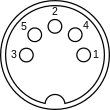
\includegraphics[scale=0.2]{Imagenes/MIDI_connector2.png}
% Ponemos Leyenda al gráfico
\caption{Conector clásico MIDI}
\label{Conector clásico MIDI}
\end{center}
\end{figure}

Optoacopladores mantienen los dispositivos MIDI eléctricamente separados de otros conectores, lo cual previene bucles de masa y protege al equipo de picos de voltage.No hay manera de detectar errores en MIDI, así que el tamaño máximo del cable es de 15 metros para limitar interferencias destructivas.

La mayoría de los dispositivos no copian los mensajes de la entrada a su puerto de salida. Un tercer tipo de puerto, el puerto ``thru'', emite una copia de todo lo que es recibido en el puerto de entrada, permitiendo que los datos sean transmitidos a otro instrumento en una ``Daisy chain''.No todos los dispositivos cuentan con un puerto thru y dispositivos que carecen de la característica de generar datos MIDI, como unidades de efectos o módulos de sonido, pueden no incluir un puerto de salida.


\paragraph{Interfaces}


La función principal de una interfaz MIDI para ordenador es sincronizar los relees entre un dispositivo MIDI y el ordenador. Algunas tarjetas de sonido de ordenador incluyen un conector MIDI estándar, mientras que en otras se conecta a través de D-sub, USB, Firewire o Ethernet. El creciente uso de conectores USB en los 2000's ha llevado a una disponibilidad de interfaces MIDI a USB que puedan transferir canales MIDI a computadoras con USB incluido. Algunos controladores MIDI están equipados con conectores USB y pueden ser conectados en ordenadores que empleen software musical.

La transmisión serial MIDI lleva a problemas de sincronización. Músicos experimentados pueden detectar diferencias de 1/3 de milisegundos (ms) (es el tiempo que tarda el sonido en viajar 4 pulgadas) y un mensaje MIDI de 3 bytes requiere 1ms para transmitirse. Debido a que el MIDI es serial, solo puede ser enviado un evento a la vez. Si un evento es enviado a dos canales a la vez, el evento con número de canal mayor no podrá ser transmitido hasta que el primero haya acabado y será retrasado 1ms. Si un evento es enviado a todos los canales al mismo tiempo, el evento con un número de canal mayor será retrasado por mucho 16ms. Esto ha contribuido a el surgimiento de interfaces MIDI con múltiples entradas y salidas debido a que la sincronización mejora cuando los eventos son enviados en diferentes puertos a diferencia de varios canales en un mismo puerto. El término ``tropiezo MIDI'' se refiere a los errores audibles resultantes de una transmisión retrasada.

\paragraph{Controladores}

Existen dos tipos de controladores MIDI: controladores para performance que generan notas y son utilizados para ejecutar música, y controladores que pueden no transmitir notas pero pueden transmitir otros tipos de eventos en tiempo real. Varios dispositivos son la combinación de los dos tipos.


\paragraph{Controladores para performance}


El MIDI fue diseñado con los teclados en mente y cualquier otro controlador que no posea un teclado es considerado como un controlador ``alternativo''. Esto ha sido visto como una limitación para los compositores que no están interesados la música que emplea teclados, la flexibilidad y compatibilidad MIDI fue introducida a otros tipos de controladores incluyendo guitarras, instrumentos de viento y cajas de ritmo.


\paragraph{Teclados}


Los teclados musicales son el tipo de controlador MIDI más común. Pueden ser encontrados en diferentes tamaños desde 25 teclas, modelos de dos octava, hasta instrumentos de 88 teclas. Algunos solo incluyen el teclado, aunque existen otros controladores en tiempo real como perillas, sliders y palancas. Usualmente existen conexiones para pedales de sustain y de expresión. La mayoría de los controladores con teclado permiten dividir el área de piano en zonas, las cuales pueden ser de diferentes tamaños y sobreponerse. Cada zona corresponde a un canal MIDI diferente y un set diferente de controladores, pueden ser usados para tocar cualquier rango de notas seleccionado. Esto permite a un solo instrumento tocar varios sonidos. Las capacidades MIDI también pueden ser encontradas en instrumentos de teclado tradicionales como pianos y pianos Rhodes. Pedaleros pueden controlar los tonos de un órgano MIDI o pueden tocar un sintetizador como el Moog Taurus.


\paragraph{Baterías y controladores de percusión}


Los teclados pueden ser utilizados para accionar sonidos de baterías pero no son prácticos para tocar patrones repetitivos como redobles debido a las dimensiones de las teclas. Después de los teclados, los pads de batería son los controladores para performance MIDI más significantes. Los controladores de percusión pueden estar integrados en cajas de ritmo, pueden ser superficies de control independientes o emular y sentirse como instrumentos de percusión. Los pads integrados en cajas de ritmos usualmente son muy pequeños y frágiles para ser tocados con baquetas, por lo que son tocados con los dedos. Drum pads especializados como el Roland Octapad o el DrumKAT son tocados con las manos o baquetas, están construidos como un set de batería. Existen otros controladores de percusión con el MalletKAT, parecido al vibráfono, y el Marimba Lumina de Don Buchla. Accionadores MIDI pueden ser instalados en una batería acústica e instrumentos de percusión. Los \gls{Pads} pueden accionar un dispositivo MIDI que puede ser casero a partir de un sensor piezoeléctrico o un pad de practica.

\paragraph{Instrumentos}

Un instrumento MIDI tiene puertos para enviar y recibir señales MIDI, un CPU para procesar dichas señales, una interfaz que permita al usuario programarlo, un circuito de audio que genere sonidos y controladores. El sistema operativo y los sonidos de fábrica usualmente están almacenados en una memoria de solo lectura (ROM).

Un instrumento MIDI también puede ser un modulo independiente (sin la necesidad de un teclado) conformado por una tarjeta de sonido General MIDI (GM, GS y /XG) editable dentro de la misma, incluyendo cambios de transport/tono, cambios de instrumento MIDI, ajuste de volumen, panel, niveles de reverberación y otros controladores MIDI. Normalmente, el modulo MIDI incluye una pantalla grande, permitiendo al usuario visualizar la información dependiendo de la función seleccionada. Otras funciones incluyen el visualizar la lírica, usualmente incluida en un archivo MIDI o Karaoke MIDI, listas de pistas, librería de canciones y pantallas de edición. Algunos módulos MIDI incluyen un armonizador y la capacidad de reproducir y reajustar archivos MP3.


\paragraph{Sintetizadores}


Los sintetizadores pueden emplear cualquier variedad de técnicas para generar sonido. Estos normalmente incluyen un teclado integrado, o pueden existir como ``módulos de sonido'' que generan sonidos a partir de un controlador externo. Los módulos de sonidos están típicamente diseñados para ser colocados en un rack de 19 pulgadas. Los fabricantes producen comúnmente un sintetizador en versiones independiente y para rack, usualmente la versión con teclado varia de tamaño.


\paragraph{Samplers}


Un sampler puede grabar y digitalizar audio, almacenarlo en una memoria de acceso aleatorio (RAM) y reproducirlo posteriormente. Los samplers normalmente permiten al usuario editar un sample y guardarlo en un disco duro, aplicarle efectos y modificar su sonido a través de las mismas herramientas usadas en los sintetizadores. También pueden tener un teclado o estar montados en un rack. Los instrumentos que generan sonidos a través de su reproducción pero que no tienen capacidades de grabación son conocidos como ``ROMplers''.

Los samplers no se convirtieron en instrumentos MIDI viables tan rápido como lo hicieron los sintetizadores debido al costo de la memoria y el poder de procesamiento en este entonces. El primer sampler MIDI de bajo costo fue el Ensoniq Mirage, lanzado en 1984. Los samplers MIDI normalmente están limitados debido a sus pequeñas pantallas empleadas para editar las formas de onda sampleadas, aunque algunos pueden ser conectados a un monitor de computadora.


\paragraph{Cajas de ritmos}


Las cajas de ritmos normalmente son dispositivos especializados que reproducen samples de batería y sonidos de percusión. Usualmente tienen un secuenciador que permite la creación de patrones ritmos para incorporarlos en el arreglo de alguna canción. Comúnmente tienen múltiples salidas que permiten que cada uno de los sonidos sea asignado a cada una. Los sonidos individuales de las baterías pueden ser reproducidos desde otro instrumento MIDI o desde un secuenciador.

\paragraph{Especificaciones técnicas}

Los mensajes MIDI están conformados de una ``palabra'' de 8 bits (llamados bytes) que son transmitidos de manera serial a 31.25 kbit/s. Esta tasa fue escogida debido a que es una división exacta de 1 MHz, la velocidad en la que varios de los primeros microprocesadores operan. El primer bit de cada palabra identifica si la palabra es un byte de estatus o de datos, los siguientes siete bits son la información. Un bit de inicio y otro de pausa son agregados a cada byte por cuestiones de sincronización, así que un mensaje MIDI requiere de diez bits para transmitirse.

Una conexión MIDI puede llevar dieciséis canales independiente de información. Los canales son numerados del 1 al 16 pero en realidad corresponden al orden del código binario del 0 al 15. Un dispositivo puede ser configurado para solo escuchar canales específicos e ignorar los mensajes enviados de otros o puede escuchar a todos los canales sin importar su dirección. Un dispositivo puede ser monofónico (el inicio de una nueva señal de ``note-on'' MIDI implica el final de la nota previa) o polifónico (múltiples notas pueden sonar al mismo tiempo, hasta que el límite de la polifonía del instrumento se haya alcanzado, las notas hayan terminado su envolvente o el comando ``note-off'' haya sido recibido. Los dispositivos que reciben los mensajes normalmente tienen cuatro combinaciones de los modos ``omni off/on'' vs. ``mono/poly''.

En la especificación técnica hay 128 Instrumentos General MIDI para el proyecto el que nos interesa es el número 10 - Caja de música.

La flexibilidad del MIDI y su gran aceptación ha llevado a varios refinamientos del estándar, además ha permitido que se aplique a propósitos más allá de los que se tenían planeados. Para ello se han diseñado extensiones al general MIDI.

\paragraph{Hardwares alternativos de transporte}

Además de la tasa de transmisión 31.25 kbit/s en un conector DIN de cinco pines, otros conectores comunes han sido usados para la misma información eléctrica y la transmisión de señales MIDI en diferentes formas a través de USB, IEEE 1394 o FireWire y Ethernet.


\paragraph{USB y FireWire}


Los miembros de USB-IF en 1999 desarrollaron un estándar para MIDI a través de USB, el ``Universal Serial Bus Device Class Definition for MIDI Devices'' El MIDI sobre el USB ha sido más común que otras interfaces que ha sido empleadas para las conexiones MIDI (serial, joystick, etc.) han desaparecido de las computadoras personales. 
Los sistemas operativos Microsoft Windows, Macintosh OS X y Apple iOS han incluido drivers para compatibilidad con ``Universal Serial Bus Device Class Definition for MIDI Devices''. Los drivers también están disponibles para Linux. Algunos fabricantes decidieron implementar una interface MIDI sobre el USB que está diseñado para operar diferente de la especificación, usando drivers personalizados.

Apple Computer desarrollo la interface FireWire durante los noventas. Comenzó a aparecer en cámaras de video digitales hacia finales de la década y en modelos de la G3 Macintosh en 1999. Fue creado para aplicaciones multimedia. A diferencia del USB, FireWire usa controladores inteligentes que pueden manejar su propia transmisión sin la atención de un CPU principal.

\paragraph{Ethernet}

La implementación del MIDI en la red de computadoras permite nuevas capacidades de conexiones y permite un canal con gran ancho de banda que las primeras alternativas de MIDI, como ZIPI, trataron de crear. Las implementaciones propietarias han existido desde los ochentas, como lo es el uso de cables fibra óptica para la transmisión.
La especificación abierta RTP MIDI del Grupo de trabajo de ingeniería de Internet está adquiriendo el apoyo de la industria debido a que los protocolos propietarios MIDI/IP requieren costos altos de licencias o no ofrecen ninguna ventaja además de la velocidad sobre el protocolo MIDI original. Apple ha apoyado este protocolo desde Mac OS X 10.4 y un driver de Windows basado en la implementación de Apple existe desde Windows XP y para las nuevas versiones.

\paragraph{Versiones de MIDI}

Una nueva versión de MIDI, llamada de manera tentativa ``Protocolo HD'' o ``High-Definition Protocol'', fue anunciada como ``HD-MIDI''. Este nuevo estándar ofrece retrocompatibilidad con el MIDI 1.0 y está planeado que soporte grandes velocidades de transmisión, permitir la detección de dispositivos con solo conectarlos, enumerarlos y ofrecer un gran rango de datos y resolución. 

Los números de los canales y los controladores aumentaran, nuevos tipos de eventos serán agregados y los mensajes serán simplificados. Nuevo eventos serán soportados como Note Update y Direct Pitch que están enfocados a controladores de guitarra. Las capas físicas propuestas incluyen protocolos basados en Ethernet como RTP MIDI y Audio Video Bridging. El protocolo HD y un protocolo de transporte basado en User Datagram Protocol (UDP) están bajo la revisión de High-Definition Protocol Working Group (HDWG) de MMA, el cual incluye a los representantes varias compañías.
Prototipos de dispositivos basados en las primeras fases del protocolo han sido mostrados de manera privada en NAMM usando tanto conexiones alambicas como inalámbricas, sin embargo es incierto si el protocolo será retomado por la industria.
En 2015, las especificaciones del protocolo HD están cerca de su finalización y MMA desarrolla las políticas de licencias y certificaciones de productos. Debido a que el costo de almacenamiento de datos ha disminuido, la música MIDI se ha visto remplazada por audio comprimido en productos comerciales, haciendo nuevamente del MIDI una herramienta para la producción musical.

La conectividad MIDI y un sintetizador de software aún se incluye en Windows, OS X y iOS pero no en Android.


\subsection{Baterías-MIDI y proyectos en entornos libre}

Visto la historia del MIDI, para entender mejor el concepto de una batería-MIDI plantearemos la idea desde crear una batería-MIDI para ir desarrollando esta bateria y luego compararla con las profesionales, de esta manera nos ayudara a entender mejor que problemas hay a la hora de desarrollar el reproductor de dtx.


\subsubsection{Arduino}


Para crear una batería simple, lo más fácil en la actualidad seria coger un microcontrolador como las placas de electrónica de Arduino. 

La primera idea más básica es coger una entrada digital de 1 bit por simplicidad y si se activa hacer que el Arduino reproduzca un sonido.
De esta manera podemos decir que tenemos una batería de 1 pad.

El primer detalle que se observaría  es que como se ha escogido una entrada digital de 1 bit nuestra batería electrónica siempre sonaría con la misma intensidad, independientemente de la intensidad que se toque al pad.

Para solucionar esto desde los años 80 se han usado unos componentes electromecánicos conocidos como sensor piezoeléctrico que es un dispositivo que utiliza el efecto piezoeléctrico para medir presión, aceleración, tensión o fuerza; transformando las lecturas en señales eléctricas.


Por tanto pasando de 1 señal digital de 1 bit, a una entrada analógica ya se tiene la posibilidad de saber la intensidad con que se ha tocado el pad.

Poniendo un sensor piezoeléctricos y conectando este a una entrada analógica, nos faltaría modificar la programación del Arduino para modificar el volumen del sonido dependiendo de la intensidad que se observa en esta entrada analógica.


El añadido siguiente es pasar a ``n'' entradas. Un detalle a tener en cuenta si la programación esta realizada para que todo sea secuencial, (que es la manera básica de programar el Arduino)  si los sonidos a reproducir son un poquito largos observaríamos que esta batería no puede hacer sonar dos \gls{Pads} al mismo tiempo.


Para resolver el problema del paralelismo a obtener en los sonidos, hay varias soluciones:
\begin{itemize}
  \item Ir a una ejecución en paralelo de nuestra idea básica de comprobar las entradas y reproducir un sonido si hay una activa.
  \item Ir a micro-controladores más potentes, para que sea más rápido a la hora de comprobar las entradas y reproducir el sonido.
  \item Separar nuestra idea de batería en dos partes una parte seria nuestro Arduino que recoge las señales de los \gls{Pads}, pero que no reproduce nada, y al tener una gran velocidad de muestreo nos podría parecer que si que esta comprobando las entradas en paralelo, y otra parte la que reproduciría los sonidos.
\end{itemize}

Como ya se ha observado en el protocolo MIDI, la idea de ir separando la generación de los eventos MIDI, con la reproducción de sonidos asociados a estos eventos MIDI, hace que pasemos a un siguiente paso de la creación de esta batería simple.


\subsubsection{Baterías-MIDI}

Ahora para continuar mejorando esta batería electrónica, lo que se debería hacer es coger un Arduino, con la posibilidad de programar una salida MIDI. 

Si se escoge un Arduino de tipo más bajo se nos daría el siguiente problema, como solo tienen un usb que se emplea para programar, o ponemos un conector extra para que haga de salida MIDI, o perdemos la opción de programar en ese usb, mientras se esta usando como salida MIDI.

Para evitar esta problemática, lo más sencillo es coger un Arduino que si que tenga la opción tener un usb para comunicarse con un ordenador sin perder el usb para programar el Arduino.

Por lo que tenemos es una batería con ``n'' \gls{Pads} con intensidad y conectándola a un sintentizador ya tenemos lo que seria una batería electrónica básica.

\begin{figure}[H]
% Centramos la figura
\begin{center}
% Incluimos el gráfico y definimos el ancho y alto
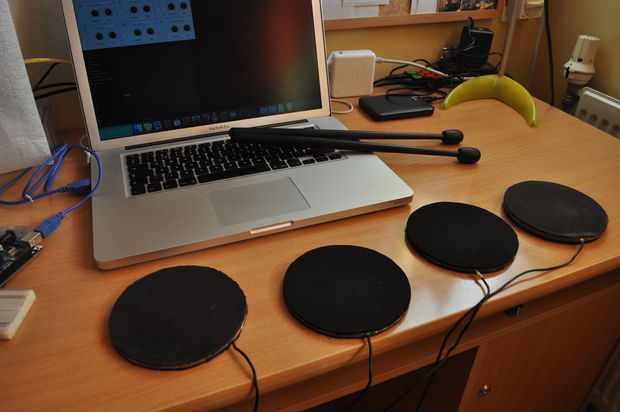
\includegraphics[scale=1.1]{Imagenes/drum-arduino.jpg}
% Ponemos Leyenda al gráfico
\caption{Ejemplo de batería electrónica de 4 pads basada en Arduino}
\label{Ejemplo de batería electrónica de 4 pads basada en Arduino}
\end{center}
\end{figure}


Aquí ya podemos establecer las diferencias con las baterías profesionales.
 

\subsubsection{Baterías-MIDI profesionales}

Evidentemente el mundo de las baterías electrónicas profesionales es muy amplio, para los objetivos de este expediente nos centraremos en las grandes diferencias que hay de esta idea básica de batería electrónica, con las baterías profesionales.

\paragraph{Baterías profesionales de entrada}

Para representar las baterías electrónicas de entrada escogemos a la Yamaha DD-65.

\begin{figure}[H]
% Centramos la figura
\begin{center}
% Incluimos el gráfico y definimos el ancho y alto
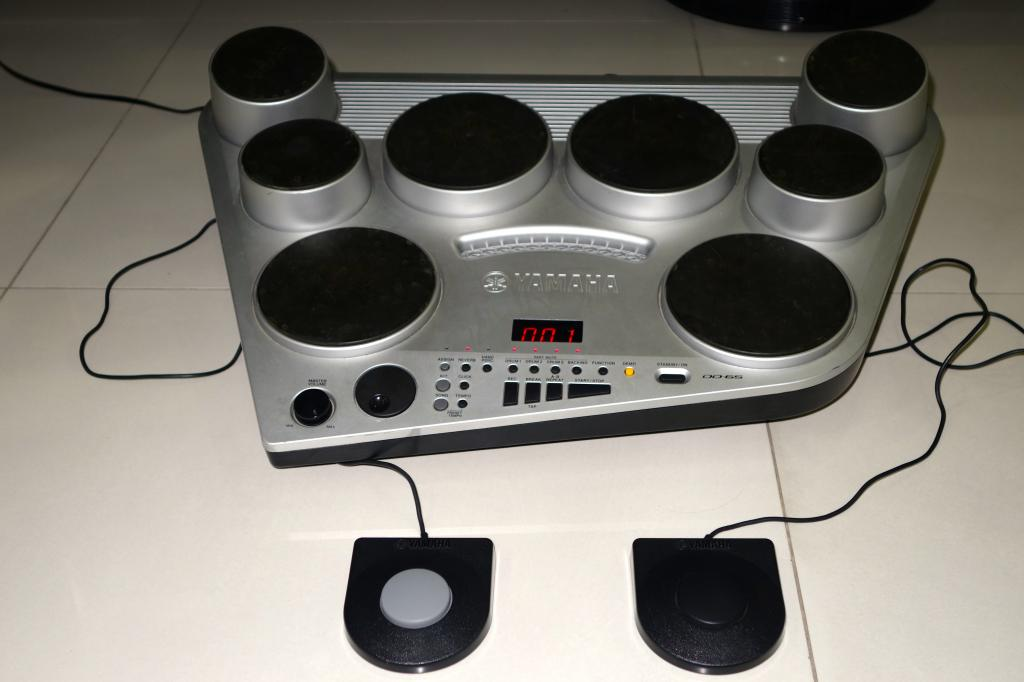
\includegraphics[scale=0.3]{Imagenes/dd-65.jpg}
% Ponemos Leyenda al gráfico
\caption{Yamaha DD-65}
\label{Yamaha DD-65}
\end{center}
\end{figure}

Como se puede observar la mayor diferencia a simple vista con la batería que se ha creado con Arduino solo es el número de \gls{Pads}, que esto hemos visto que tiene fácil solución.

Otra diferencia son los dos pedales, se podría pensar en la misma solución poner dos \gls{Pads} más y ponerlos en el suelo para activarlos con los pies. No parece que sea un gran problema a no ser que recordemos como funciona una batería real.

El hihat es un instrumento de batería que tiene un pedal asociado, este instrumento suena distinto según su pedal las dos posiciones basicas del pedal son abierto o cerrado, por lo que en nuestra batería tendríamos que actuar en consecuencia, esto solo es un detalle de programación a la hora de enviar el evento MIDI asociado al pad del hihat, ya que se tiene que enviar un evento distinto si esta el pedal pulsado o no.

En esta batería se pueden conectar otros pedales para hihat y bombo que se asemejen más a unos reales.

Esta batería tiene 254 sonidos y 50 baterías predefinidas con ellos, de todas manera se puede configurar 3 baterías con cualquiera de esos 254 sonidos, pero no se puede modificar ninguno de estos sonidos, Yamaha con este tipo de batería quiere ofrecer al público una batería portátil e independiente que sea configurable por el usuario, y para que sea portable se ha de separar de lo que sería una batería acústica en cuanto al aspecto físico.


Yamaha con esta batería lo que quiere hacer es una batería electrónica por un precio mínimo. Yamaha indica que esta batería es independiente por lo que se puede tocar sin tener que conectar a un ordenador. Aquí una de las mayores problemáticas que existe a la hora de afrontar que es una batería electrónica, ya que hay gente que entiende que se tiene que simular lo más cercano a una batería acústica, mientras que hay otro razonamiento que ya que se esta delante de un instrumento electrónico se ha de aprovechar todas las posibilidades que esto nos da aunque se separe de lo que es una batería clásica.


\paragraph{Baterías semiprofesionales}

 A mayor precio ya tenemos la gama de Roland V-Drums Lite
 
\begin{figure}[H]
% Centramos la figura
\begin{center}
% Incluimos el gráfico y definimos el ancho y alto
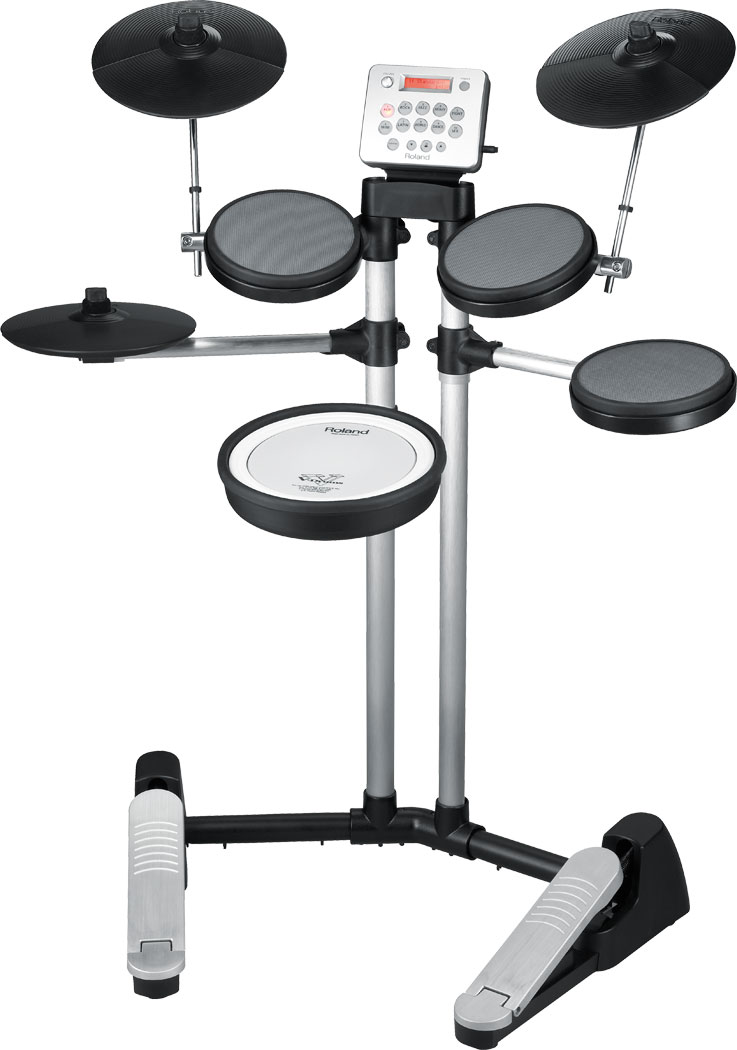
\includegraphics[scale=0.2]{Imagenes/V-Drums_Lite_HD-3.jpg}
% Ponemos Leyenda al gráfico
\caption{Roland V-Drums Lite HD-3}
\label{Roland V-Drums Lite HD-3}
\end{center}
\end{figure}

Se puede observar en esta batería la misma idea que la anterior pero físicamente más parecida a una batería real para que si alguien se acostumbra a tocar en esta batería, el cambio a una batería acústica sera mucho menor.

En esta batería tiene 20 baterías predefinidas y no da la posibilidad de modificarlas en su propio sintetizador, Roland supone que si se quiere modificar la batería se hará a través del canal MIDI-out en otro sintetizador(u ordenador).

En esta batería físicamente no se pueden modificar los \gls{Pads} ni los pedales ya que están soldados los cables que van al sintetizador.


\paragraph{Baterías profesionales}

 A mayor precio ya tenemos la gama de Roland V-Drums T, ponemos por ejemplo la TD-30.
 
\begin{figure}[H]
% Centramos la figura
\begin{center}
% Incluimos el gráfico y definimos el ancho y alto
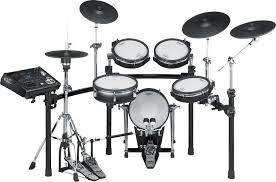
\includegraphics[scale=0.7]{Imagenes/td-30.jpg}
% Ponemos Leyenda al gráfico
\caption{Roland TD-30}
\label{Roland TD-30}
\end{center}
\end{figure}

Se puede observar que han aumentado el número de platillos, el hihat es más parecido a uno real e incluso tiene 3 pedales para tener el doble bombo y el hihat, separados e independientes.

Pero evidentemente hay mucho más, internamente la calidad del sonido que reproduce por ella misma se ha ido aumentado.

Aunque los \gls{Pads} que hacen de platillos parecen igual que los segundos y podríamos pensar que es la misma idea que nuestra batería construida con el Arduino, esta batería tiene en los platillos varios piezos para poder configurarlos de varias maneras.
La más simple es que según se detecte el piezo más superior o el del borde sonara un sonido distinto, siendo más cercano a lo que sonaría en una batería acústica.
Otra manera de configurar estos platillos es que si se toca el piezo más cercano al borde para el sonido de los otros piezos, imitando lo que pasa si se cogiera un platillo real con las manos, para hacer que deje de vibrar.

En esta batería se puede modificar tanto los samples que ha de usar cada pad o piezo.

Al tener un sintetizador totalmente independiente, también se puede modificar los pads o pedales, por otros más a gusto del percusionista.
 
\paragraph{Conclusiones}
Tal y como se ha ido exponiendo, se va a resumir las principales características por las cuales se puede diferenciar una bateria-MIDI de otra y de esta manera tener un concepto más claro de que se podrá conectar a nuestro proyecto.

La principal idea es que se ha de aproximar en la medida de lo posible a una batería acústica, por lo que independientemente o no, se tiene que poder escuchar sonidos asociados a los impactos que hagamos en los pads.

Las principales características de una batería electrónica a tener en cuenta este proyecto son:
\begin{itemize}
  \item Todas tienen salida MIDI.
  \item Número de \gls{Pads} y colocación de estos.
  \item Número de entradas dedicadas a los pedales.
  \item La capacidad de modificar los samples internos que tienen.
  \item La capacidad de modificar su funcionamiento interno.
\end{itemize}

\subsection{Actualidad de Reproductores DTXMania en entornos libres}

Se va a exponer el estado actual de los juegos DTXmania y DTXmaniaXG en entornos libres.

Todos estos programas están programados para la plataforma PC, pero entendiendo PC como Windows evidentemente plataforma x86 y como es un japones el que los esta programando usando características de Windows en Japón.

Desde hace bastante tiempo dejo el programa como software libre, la página web del programa se puede consultar en:

\url{https://osdn.jp/projects/dtxmania/} 


El mismo autor tiene el programa DTXmaniaXG, para emular los programas DrumMania XG y Gitadora.

\url{https://osdn.net/projects/dtxmaniaxg-verk/}

La gran mayoría de la documentación estando en perfecto japones.

Aunque siempre esta la opción de maquinas virtuales, estamos hablando de juegos musicales donde tanto el tema de la latencia en eventos MIDI hacia el programa como la sincronización del sonido es muy importante, por lo que esta opción es valida mientras estemos pensando en ejecutarlo en una maquina bastante potente.

La otra gran opción es usar WINE, pero aunque se ponga las opciones de lenguaje en japones, parece que no llega a crear bien o acceder a los archivos por problemas de codificación del lenguaje japones y sistema de ficheros por lo que no se llega ni acceder al menú inicial, de cualquiera de estos programas  (Versión probada de wine 2.5).

Pero también hay que pensar para otros entornos (arm/MIPS/RISCv), y ninguna de estas dos opciones son viables fácilmente para otras plataformas que no sean x86.

Hubo un proyecto antiguo llamado DigiBand el cual era un simulador/juego de baterías en entornos libres, que podía funcionar con canciones con el formato DTX, este programa tiene varios inconvenientes.
\begin{itemize}
  \item En el 2005 fue la última vez que alguien modifico el código fuente.
  \item Emplea librerías que ya en 2005 estaban deprecated.
\end{itemize}

Se ha intentado compilarlo tanto en entorno x86-64, usando un fedora 25 para ello, como en un entorno arm usando una Raspberry. Y no se ha podido compilar, tanto por las dependencias antiguas que tiene como por los cambios en las librerías que se han sucedido en estos 12 años.

\subsubsection{Otros juegos musicales}

Como muchos juegos musicales, comparten la base,por lo que vamos a mostrar que existe en la actualidad para poder afianzar la base en la que trabajar.


Los juegos de \gls{Rock Band} salieron para consolas pero no llegaron a salir para PC, por lo que  ya no digamos plataformas en entornos libres.

Hay un juego que se considera el nuevo sucesor espiritual del \gls{Rock Band} para PC, que es el PhaseShift misma idea pero gráficos más actualizados, usando como base:

\begin{itemize}
  \item Windows XP/ Vista / 7
  \item DirectX 9.0c
  \item VC++ Redist
\end{itemize}

Y cuando se les pregunta a los autores de PhaseShift por MAC o linux, contestan:
\begin{itemize}
  \item Q. Will you add support for Mac / Linux
  \item A. We do not have the resources to develop native versions, but the game is now compatible with Wine / Crossover.
\end{itemize}

Por lo que se deduce es que se podría llegar a tener en entornos ``libres'' usando WINE por lo que se puede entender que se pueden ejecutar si la maquina tiene la potencia suficiente.

El juego FoFiX como salio de un proyecto (Frets on fire) que era libre, no fue muy difícil modificarlo para que funcionar en entornos libres.
En entornos x86 no tiene mayor inconveniente el problema esta en los entornos arm que al no soler tener OpenGL, no funciona. Indicar que en el entorno de la Raspberry pi, tanto en la 2 como en la 3 activando el driver beta OpenGL, comienza a funcionar, pero no se llega a ver todo bien y todavía hay muchos flecos a resolver en el driver de OpenGL.


El juego Dance Dance Revolution como hemos comentado antes si que tiene una versión libre, el StepMania en esa versión le pasa lo mismo que al FoFiX en plataformas x86, funciona bien pero cuando nos pasamos a entornos arm es cuando hay problemas con toda la parte gráfica ya que emplea OpenGL.

Aunque existe un juego llamado PyDance que emplea librerías de muy bajo nivel, lo que hace que tenga menús muy simplificados y poca carga gráfica mientras se juega a DDR se puede hacer funcionar tanto en entornos x86 como arm sin necesidad de tener OpenGl. Eso si esta pensado para canciones de tipo DDR no DTXMANIA.  Emplearemos este programa como base para poder entender que tenemos que hacer para crear un reproductor de canciones .dtx en entornos libres.

Por lo que vemos el estado de los juegos musicales en entornos libres no es totalmente malo, pero son proyectos en los que la plataforma principal y casi se podría decir que única ha sido la x86, aunque dejando la puerta abierta a otras plataformas.


\subsection{Raspberry}

Como se ha observado casi siempre la plataforma principal ha sido la plataforma x86 para esto tipos de juegos musicales, ahora vamos a hacer un repaso a otra plataforma que esta cogiendo mucha fuerza en la actualidad, para ello expondremos el principal ordenador, con plataforma tipo arm que a nivel educativo esta cambiando la manera de entender los ordenadores.

Raspberry PI es un ordenador de placa reducida o (placa única) (SBC) de bajo coste, se podría decir que es un ordenador de tamaño reducido, del orden de una tarjeta de crédito, desarrollado en el Reino Unido por la Fundación Raspberry PI (Universidad de Cambridge) en 2011, con el objetivo de estimular la enseñanza de la informática en las escuelas, aunque no empezó su comercialización hasta el año 2012.

Aunque no se indica expresamente si es hardware libre o con derechos de marca, explican que disponen de contratos de distribución y venta con dos empresas, pero al mismo tiempo cualquiera puede convertirse en revendedor o redistribuidor de las tarjetas RaspBerry Pi, por lo que se entiende que es un producto con propiedad registrada pero de uso libre. De esa forma mantienen el control de la plataforma pero permitiendo su uso libre tanto a nivel educativo como particular.


En cambio el software sí es open source, siendo su sistema operativo oficial una versión adaptada de Debian, denominada RaspBian, aunque permite otros sistemas operativos, incluido una versión de Windows 10.

El concepto es el de un ordenador desnudo de todos los accesorios que se pueden eliminar sin que afecte al funcionamiento básico. Está formada por una placa que soporta varios componentes necesarios en un ordenador común y es capaz de comportarse como tal.

El diseño de la Raspberry Pi 1 u original incluye:

\begin{itemize}
  \item Un Chipset Broadcom BCM2835, que contiene un procesador central (CPU) ARM1176JZF-S a 700 MHz (el firmware incluye unos modos Turbo para que el usuario pueda hacerle overclock de hasta 1 GHz sin perder la garantía).
  \item Un procesador gráfico (GPU) VideoCore IV.
  \item Un módulo de 512 MB de memoria RAM (aunque originalmente al ser lanzado eran 256 MB).
  \item Un conector de RJ45 conectado a un integrado lan9512 -jzx de SMSC que nos proporciona conectividad a 10/100 Mbps
  \item 2 conexiones USB 2.0
  \item Una Salida analógica de audio estéreo por Jack de 3.5 mm.
  \item Salida digital de video + audio HDMI
  \item Salida analógica de video RCA
  \item Pines de entrada y salida de propósito general
  \item Conector de alimentación microUSB
  \item Lector de tarjetas SD
\end{itemize}


\subsubsection{Historia} 
Este proyecto fue ideado en 2006 pero no fue lanzado al mercado febrero de 2012. Ha sido desarrollado por un grupo de la Universidad de Cambridge y su misión es fomentar la enseñanza de las ciencias de la computación los niños. De hecho, en enero de este año Google donó más de 15.000 Raspberry Pi para colegios en Reino Unido. La Raspberry Pi, es una excelente herramienta para aprender electrónica y programación.

Los primeros diseños de Raspberry Pi se basaban en el microcontrolador Atmel ATmega644. Sus esquemas y el diseño del circuito impreso están disponibles para su descarga pública.

La fundación Raspberry Pi surge con un objetivo en mente: Desarrollar el uso y entendimiento de los ordenadores en los niños. La idea es conseguir ordenadores portables y muy baratos que permitan a los niños usarlos sin miedo, abriendo su mentalidad y educándolos en la ética del ``ábrelo y mira cómo funciona''. El ideólogo del proyecto, David Braven, un antiguo desarrollador de videojuegos, afirma que su objetivo es que los niños puedan llegar a entender el funcionamiento básico del ordenador de forma divertida, y sean ellos mismos los que desarrollen y amplíen sus dispositivos. El co-fundador de la fundación es Eben Upton, un antiguo trabajador de la empresa Broadcom, el cual es el responsable de la arquitectura de software y hardware de la raspberry pi.

Eben Upton, se puso en contacto con un grupo de profesores, académicos y entusiastas de la informática para crear un ordenador con la intención de animar a los niños a aprender informática como lo hizo en 1981 el ordenador Acorn BBC Micro.

La fundación da soporte para las descargas de las distribuciones para arquitectura ARM, Raspbian (derivada de Debian), RISC OS y Arch Linux; y promueve principalmente el aprendizaje del lenguaje de programación Python, y otros lenguajes como Tiny BASIC, C y Perl.

El primer prototipo basado en ARM fue montado en un paquete del mismo tamaño que una memoria USB. Tenía un puerto USB en un extremo y un puerto HDMI en el otro.

En agosto de 2011, se fabricaron cincuenta placas Alpha del modelo inicial, el Model A (o modelo A). En diciembre de 2011, 25 placas Beta del modelo B fueron ensambladas y probadas de un total de 100 placas vacías.

Durante la primera semana de diciembre de 2011, se pusieron a subasta diez placas en eBay. Debido al anticipado anuncio de puesta a la venta a final de febrero de 2012, la fundación sufrió colapso en sus servidores web debido a los refrescos de páginas desde los navegadores de gente interesada en la compra de la placa.

El primer lote de 10.000 placas se fabricó en Taiwán y China, en vez de Reino Unido, con esto se conseguía un abaratamiento en los costes de producción y acortar el plazo de entrega del producto, ya que, los fabricantes chinos ofrecían un plazo de entrega de 4 semanas y en el Reino Unido de 12. Con este ahorro conseguido, la fundación podía invertir más dinero en investigación y desarrollo.

Las primeras ventas comenzaron el 29 de febrero de 2012 (Modelo B). Las dos tiendas que vendían las placas, Premier Farnell y RS Components, tuvieron una gran carga en sus servidores inmediatamente después del lanzamiento. En los seis meses siguientes llegarían a vender  500.000 unidades.

El 16 de abril de 2012 los primeros compradores empezaron a informar que habían recibido su Raspberry Pi. El 22 de mayo de 2012 más de 20.000 unidades habían sido enviadas.

El 6 de septiembre se anunció que se llevaría la producción de placas al Reino Unido, a una fábrica de Sony y que en ella se producirían 30.000 unidades cada mes, y se crearían 30 nuevos puestos de trabajo.

El 4 de febrero de 2013, se lanzó el modelo A, que venía con solo 256Mb de RAM y sin puerto ethernet a un precio más asequible que el modelo B.

En diciembre de 2015 se pueden comprar modelos con mejores prestaciones; Raspberry Pi 2 Model B - Placa base (ARM Quad-Core 900 MHz, 1 GB RAM, 4 x USB, HDMI, RJ-45) de Raspberry Pi, manteniendo el precio de la Raspberry original.


En febrero de 2016 sale a la venta un nuevo modelo, la versión 3 con las siguientes características: ARM Quad-Core 1,2 GHz, 1 GB RAM, 4 x USB, HDMI, RJ-45 y una conectividad inalámbrica integrada de 802.11 b/g/n LAN y Bluetooth, se continua manteniendo el precio original.

\subsubsection{Hardware}
El modelo A solo tiene un puerto USB, carece de controlador Ethernet y cuesta menos que el modelo B, el cual tiene dos puertos USB y controlador Ethernet 10/100. En 2014 se lanzó el modelo Raspberry Pi 2 B. El modelo lanzado en 2015 es el Raspberry Pi Zero. Y en 2016 se ha lanzado el modelo Raspberry Pi 3 B.


A pesar que el Modelo A no tiene un puerto RJ45, se puede conectar a una red usando un adaptador USB-Ethernet suministrado por el usuario. Por otro lado, a ambos modelos se puede conectar un adaptador Wi-Fi por USB, para tener acceso a redes inalámbricas o internet. El sistema cuenta con 256 MB de memoria RAM en su modelo A, y con 512 MB de memoria RAM en su modelo B. Como es típico en los ordenadores modernos, se pueden usar teclados y ratones con conexión USB compatible con Raspberry Pi.

El Raspberry Pi no viene con reloj en tiempo real, por lo que el sistema operativo debe usar un servidor de hora en red, o pedir al usuario la hora en el momento de arrancar el ordenador. Sin embargo se podría añadir un reloj en tiempo real (como el DS1307) con una batería mediante el uso de la interfaz I2C.


La aceleración por hardware para la codificación de vídeo (H.264) se hizo disponible el 24 de agosto de 2012, cuando se informó que la licencia permitiría su uso gratuitamente; antes se pensó en anunciarlo cuando se lanzara el módulo de cámara.También se puso a la venta la capacidad para poder usar el codificación-decodificación de MPEG-2 y Microsoft VC-1. Por otro lado, se hizo saber que el ordenador soportaría CEC, permitiendo que pudiera ser controlado mediante un mando a distancia de televisión.

El 5 de septiembre de 2012, se anunció una revisión 2.0 de la placa, que ofrecía un pequeño número de correcciones y mejoras, como unos agujeros de montaje, un circuito para hacer reset, soporte para depuración JTAG, etc.

El 15 de octubre de 2012, la fundación anunció que todos los Raspberry Pi Modelo B serían enviados a partir de ese momento con 512 MB de RAM en vez de 256 MB.

El ``system on a chip'' (SoC) usado en la primera generación de la Raspberry Pi es equivalente más o menos a los chips usados en los smartphones viejos (como el iPhone, 3G, 3GS). La Raspberry Pi esta basada en el SoC de Broadcom BCM2835 , que incluye un procesador ARM1176JZF-S a  700 MHz, una cpu gráfica VideoCore IV (GPU), y RAM. 

La Raspberry Pi 2 tiene un Broadcom BCM2836 SoC  con un procesador quad-core ARM Cortex-A7 a 900 MHz de 32-bit, con 256 KB de cache L2 compartida.

La Raspberry Pi 3 tiene un Broadcom BCM2837 SoC  con un procesador quad-core ARM Cortex-A7 a 1.2 GHz de 64-bit, con 512 KB de cache L2 compartida.

\begin{figure}[H]
% Centramos la figura
\begin{center}
% Incluimos el gráfico y definimos el ancho y alto
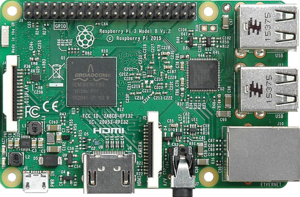
\includegraphics[scale=0.5]{Imagenes/Raspberry_Pi_3_Model_B.png}
% Ponemos Leyenda al gráfico
\caption{Raspberry Pi 3 B}
\label{Raspberry Pi 3 B}
\end{center}
\end{figure}

\subsubsection{Software}
El Raspberry Pi usa mayoritariamente sistemas operativos basados en el núcleo Linux. Raspbian, una distribución derivada de Debian que está optimizada para el hardware de Raspberry Pi, se lanzó durante julio de 2012 y es la distribución recomendada por la fundación para iniciarse.

A la GPU se accede mediante una imagen del firmware de código cerrado, llamado blob binario, que se carga dentro de la GPU al arrancar desde la tarjeta SD. El blob binario está asociado a los drivers Linux que también son de código cerrado. Las aplicaciones hacen llamadas a las librerías de tiempo de ejecución que son de código abierto, y estas librerías hacen llamadas a unos drivers de código abierto en el kernel de Linux. La API del driver del kernel es específica para estas librerías. Las aplicaciones que usan vídeo hacen uso de OpenMAX, las aplicaciones 3D usan OpenGL ES y las aplicaciones 2D usan OpenVG; OpenGL ES y OpenVG hacen uso de EGL y éste último, del driver de código abierto del kernel.

El 24 de octubre de 2012, Alex Bradbury, director de desarrollo Linux de la fundación, anunció que todo el código del driver de la GPU Videocore que se ejecuta en ARM sería de código abierto, mediante licencia BSD modificada de 3 cláusulas. El código fuente está disponible en un repositorio de la fundación en GitHub.

El 5 de noviembre de 2012, Eben Upton anunció el lanzamiento del sistema operativo RISC OS 5 para Raspberry Pi a la comunidad, pudiéndose descargar la imagen de forma gratuita desde la web de la fundación. Su relación con la comunidad RISC OS se remontaba a julio de 2011, cuando habló en ella de una hipotética versión.

El 24 de noviembre de 2012, se anunció en la Minecon de París, el juego Minecraft: Pi Edition para Raspberry Pi, basado en la versión Minecraft: Pocket Edition para teléfonos inteligentes y tabletas.La descarga se hizo disponible de forma oficial y gratuita por primera vez el 12 de febrero de 2013 desde el blog del juego, como versión 0.1.1 alpha, junto a instrucciones para ejecutarlo en Raspbian Wheezy. Una de las características principales de este lanzamiento es poder interaccionar con el juego mediante programación, con la intención de motivar a los niños a aprender a programar.

El 25 de mayo de 2013, la fundación informó de que se estaba trabajando en una versión del servidor gráfico Wayland para Raspberry Pi, para sustituir al sistema de ventanas X. Con este cambio se lograría suavidad al usar la interfaz gráfica del escritorio, ya que el procesamiento lo realizaría la GPU Videocore y no la CPU, sin interferir en el renderizado 3D.

El 3 de junio de 2013, fue lanzado en la web de la fundación para su descarga la aplicación NOOBS (New Out of Box Software), utilidad que facilita la instalación de diferentes sistemas operativos para Raspberry Pi. Se distribuye en forma de archivo zip que se copia descomprimido a una tarjeta SD de 4 GB o superior, y una vez arrancada la placa con la tarjeta por primera vez, aparece un menú en que se da la opción de instalar una de las diferentes distribuciones en el espacio libre de la tarjeta de memoria, o acceder a internet con el navegador Arora integrado. 

El 26 de septiembre de 2013, se añadió a los repositorios de Raspbian una versión oficial de Oracle Java JDK ARM con soporte para coma flotante por hardware, que ofrece bastante más rendimiento que la versión OpenJDK ARM ya existente hasta ese momento y más compatibilidad con aplicaciones. También se anunció que esta versión de Oracle Java JDK se incluiría dentro de la distribución en futuras versiones de Raspbian.


\subsubsection{Accesorios}
\paragraph{Cámara}

 El 14 de mayo de 2013, la fundación y los distribuidores RS Components \& Premier Farnell/Element 14 lanzaron la cámara para la Raspberry Pi con una actualización del firmware para que funcionara. 
Se conecta al puerto CSI de la placa mediante un cable plano flexible. El precio es de unos 20\euro{}, puede capturar video a 1080p, 720p y 640x480p. Sus dimensiones son de 25 mm x 20 mm x 9 mm.
\paragraph{Gertboard}

Este accesorio aunque no es de la fundación, ha tenido el visto de bueno de ellos, diseña con propósitos para la educación, expande los GPIO para poder interactuar con LED's, switches, señales analógicas, sensores y otros dispositivos. También incluye un controlador opcional para Arduino para poder interaccionar con el Raspberry Pi.
 
\paragraph{Cámara de infrarojos}
A finales de octubre de 2013 se puso a la venta un módulo de cámara de infrarrojos, llamada la Pi NoIR.

\paragraph{HAT}

HAT (Hardware Attached on Top) , placas de expansión, junto al modelo B+, inspiradas en las placas de expansión del Arduino, el interface para las HAT fue definido por la fundación Raspberry Pi. Cada HAT tiene que tener una pequeña EEPROM( suelen llevar la CAT24C32WI-GT3) conteniendo los detalles importantes de la placa, de tal manera que el sistema operativo de la Raspberry Pi tiene el conocimiento del HAT, y de sus aspectos tecnicos importantes para el sistema operativo de como interactuar con el HAT.
Las especificaciones mecanicas de un HAT, es que tiene que usar los cuatro agujeros en su formación rectangular.

De esta manera la fundación dejo como se podía ir ampliando el proyecto Raspberry.


Aunque hay muchas placas para expandir la Raspberry vamos a comentar brevemente tres que vemos muy interesante para este proyecto.

\paragraph{DAC}
La calidad del sonido obtenido por la Raspberry depende directamente de la tarjeta de sonido a la que conectemos, la Raspberry Pi tiene dos grandes opciones:

La primera y por defecto es la salida HDMI de esta manera es el monitor y su amplificador el responsable de la calidad final del sonido.

La segunda es la salida analogica que tiene la Raspberry, esta opción no tiene demasiada calidad, pero se ha de pensar en el precio de la Raspberry.
Mucha gente se quejaba de que el sonido no era de gran calidad cuando era la Raspberry la encargada de procesar el sonido para ello salieron varios HATs para que la Raspberry pudiera procesar sonido de alta calidad.

Estas soluciones suelen ser mejores que poner una tarjeta de sonido por USB ya que además de estar seguros que funcionara en la Raspberry, suelen emplear el protocolo I2S para reducir el uso de la CPU.

\paragraph{PianoHAT}

Aquí tenemos un HAT que integra 13 teclas en la disposición de un piano de una octava completa. Y 3 teclas más para modificar este piano.

Juntando esta HAT con una Raspberry se puede tocar el piano en la misma Raspberry. 
Los fabricantes de este HAT han publicado unos programas en el lenguaje Python para que este HAT saque comandos MIDI a través del USB y conectarlo a cualquier sintentizador. 

Este HAT respeta las libertades del usuario, y tiene tanto el hardware como el software abierto y documentado para modificarlo como uno quiera.

\begin{figure}[H]
% Centramos la figura
\begin{center}
% Incluimos el gráfico y definimos el ancho y alto
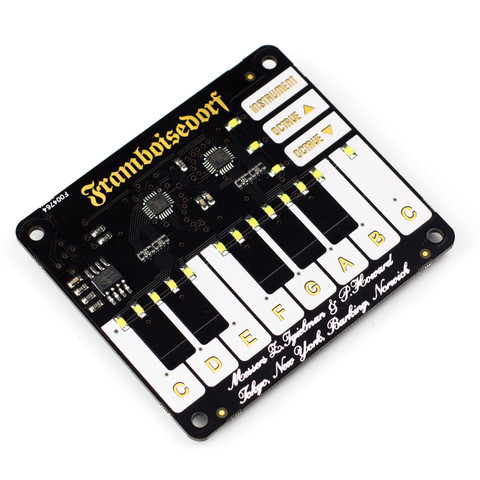
\includegraphics[scale=0.5]{Imagenes/Piano_HAT.jpg}
% Ponemos Leyenda al gráfico
\caption{Piano HAT}
\label{Piano HAT}
\end{center}
\end{figure}



\paragraph{DrumHAT}

Pimoroni los fabricantes del PianoHat viendo su exito se decidieron a hacer lo mismo pero con una batería en vez de un piano de esta manera nació el DrumHAT.

\begin{figure}[H]
% Centramos la figura
\begin{center}
% Incluimos el gráfico y definimos el ancho y alto
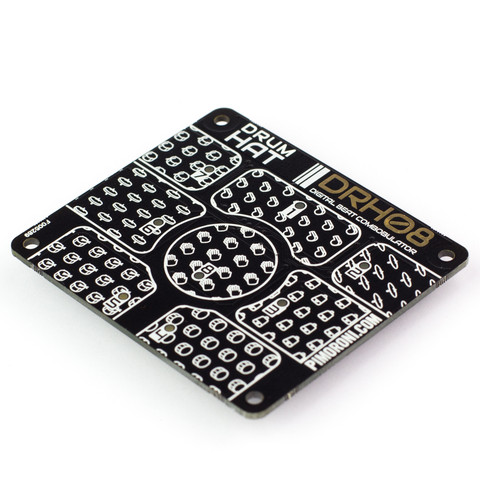
\includegraphics[scale=0.5]{Imagenes/Drum_HAT.jpg}
% Ponemos Leyenda al gráfico
\caption{Drum HAT}
\label{Drum HAT}
\end{center}
\end{figure}

Aunque ha tenido un relativo éxito, no ha tenido tanto como el pianoHat, recordar que el instrumento-MIDI por defecto es el piano, por lo que aunque en teoría es posible los fabricantes no han dado la opción para que el DrumHAT pueda sacar eventos MIDI.

\subsubsection{Comunidad}

La comunidad de Raspberry Pi fue descrita por Jamie Ayre de la compañía AdaCore ligada a FLOSS como una de las partes más excitantes del proyecto. El blogger de la comunidad Russell Davis, dijo que gracias a la fuerza de la comunidad, la fundación puede concentrarse en la documentación y la enseñanza.

Una serie de eventos llamados Raspberry Jam, dirigidos por Alan O’Donohoe han sido organizados en el Reino Unido, y en otras partes del mundo, para involucrar a la gente con la comunidad.

Desde mayo de 2012 es publicada mensualmente una revista gratuita llamada MagPi, que se dedica divulgar información acerca del Raspberry Pi, e incluye proyectos que se pueden desarrollar con él y cursos de programación de diferentes lenguajes. Es publicada mediante licencia Creative Commons BY-SA-NC.

El 2 de agosto de 2012, se añadió al foro oficial de la fundación los subforos en español, portugués y alemán (el de francés ya llevaba tiempo creado).

El 17 de diciembre de 2012, junto a la versión 2012-12-16-wheezy-raspbian de Raspbian, se lanzó la tienda de aplicaciones ``Pi Store'', que en el momento de salida incluía desde aplicaciones como LibreOffice o Asterisk a juegos como Freeciv o OpenTTD. En esta plataforma se puede poner a disposición de todos los usuarios de Raspbian, mediante moderación y posterior lanzamiento, contenidos gratuitos o de pago, como archivos binarios, código python, imágenes, audio o vídeo. Además se quiere incluir documentación acerca del Raspberry Pi como la revista MagPi y tutoriales de proyectos.

\subsubsection{Recepción e influencia}

El escritor sobre tecnología, Glyn Moody, describió el proyecto en mayo de 2011 como un ``potencial BBC Micro 2.0'', no para reemplazar a los ordenadores personales sino como algo suplementario. Alex Hope, coautor de Next Gen Report, sentía esperanzas de que el Raspberry Pi animaría a los niños a aprender a programar, en vez de a usar aplicaciones ya creadas. El coautor Ian Livingstone sugirió que la BBC podría involucrarse en el proyecto, con la posibilidad de hacerlo llamar ``BBC Nano''. Chris Williams que escribe en The Register, ve la inclusión de lenguajes de programación como Kids Ruby, Scratch y Basic como un ``buen comienzo'' para dar a los niños habilidades que necesitarán en el futuro, pero que habrá que ver cómo de efectivo será su uso. El Centro de la historia de la computación da un fuerte apoyo al proyecto y sugiere que podría ``marcar el comienzo de una nueva era''. Antes del lanzamiento del Raspberry Pi, la placa fue mostrada por el CEO de ARM, Warren East, en un evento en Cambridge, haciendo referencia a la filosofía de Google de mejorar la enseñanza de ciencias y tecnología de la computación en el Reino Unido.

Harry Fairhead sugiere que se tendría que dar más énfasis en mejorar el software educacional en el hardware actual, usando herramientas como Google App Inventor, para volver a enseñar programación en las escuelas, en vez de sacar nuevos sistemas. 


En octubre de 2012 el Raspberry Pi ganó el premio T3 ``Innovación del año''.

\subsubsection{SonicPi}

Aunque el formato MIDI es el más usado por los músicos me gustaría añadir un pequeño aporte, a nuevas formas de crear, editar y escuchar música en entornos libres.

Se ha creado el lenguaje musical SonicPi en el cual es más parecido a programar que a enfrentarse a una partitura clásica. El proyecto Raspberry Pi lo ha cogido como una de sus ramas para que los jóvenes aprendan música y esto se merece un pequeño punto en este proyecto.


\subsubsection{Usos}

En enero de 2012, encuestas hechas en el Reino Unido acerca de la penetración en las aulas de Raspberry Pi concluyeron que por cada placa que había en un colegio público, había cinco en colegios privados. Por ello se espera que en un futuro empresas patrocinen la adquisición de placas en colegios públicos.

El CEO de Premier Farnell declaró que el gobierno de un país de medio oriente expresó interés en proveer una placa a cada chica estudiante, con el objetivo de mejorar sus expectativas de empleo en el futuro.

A finales de enero de 2013, se dio a conocer que Google, junto con la ayuda de otros 6 socios, repartiría 15.000 placas entre estudiantes del Reino Unido que mostraran motivación por las ciencias de la computación.


Visto todo esto vemos ahora podemos definir el proyecto en mejores condiciones.

\chapter{Proyecto de canciones DTXMANIA entorno libre}
\section{Planteamiento general}
El planteamiento general es crear un reproductor de canciones del DTXMANIA, DTXMANIA HD y GITADORA en entornos libres.

Para ello se ha decidido usar tanto la Raspberry Pi 3 como principal plataforma arm con la distribución Raspbian y también la plataforma x86-64 con la distribución Fedora.

Para que el proyecto tenga más interés para los baterías reales este proyecto deberá mantener  la principal características del DTXMANIA original, como poder conectar Baterías-MIDI y usar estas para tocar las canciones.

Ya que se ha optado para crear el reproductor de canciones dtx en arquitecturas x86 y arm, por lo que no deberíamos usar características especificas de una plataforma de esta manera se dejara abierto para que en otras posibles plataformas ya sea MIPs o RISCv respetando las librerias que se emplean, debería poder funcionar en ellas. 

Todo el proyecto estará bajo la licencia GPL3.0, y se intentara que todas las librerias usadas también respeten estas libertades.

También se hará compatible con el Drum HAT de Pimoroni, para poder tener el proyecto conservando la filosofía de educación de la Raspberry Pi.

Por lo que los principales objetivos del proyecto se podrían resumir en los siguientes.
\begin{itemize}
\item Dar una posibilidad a los baterías a usar estas en entornos abiertos, como simulación/juego.
\item Conseguir que la comunidad de los entornos libres continué creciendo.
\end{itemize}

El reproductor de canciones dtx tendrá que conservar algunas de sus principales características.

Muy importantes:
\begin{itemize}
  \item Poder conectar baterías-MIDI y configurar estas para su uso en el reproductor.
  \item Poder configurar la velocidad de sincronización de las notas.
  \item Poder configurar el reproductor para poder poner en automático algunas lanes por si la batería-MIDI no tuviera suficientes pads o por si no queremos/sabemos tocar esa parte.
  \item Poner una base para estudiar y mejorar la percusión en entornos abiertos.
\end{itemize}

Importantes:
\begin{itemize}
  \item Si una canción tiene varias dificultades poder escoger que dificultad se quiere reproducir.
  \item Tener temas de interfaz, por si el interfaz por defecto no gusta.
  \item Tener una puntuación para saber lo bien o mal que se ha tocado.
  \item Se tiene que poder modificar el uso del reproductor de tal manera que si nuestra batería-MIDI tiene muchos pads y pedales se tiene que poder dejar de tal manera que el reproductor nos obligue a tocar lo más cercano a una batería acústica.
\end{itemize}

Se ha de tener en cuenta que al ser un proyecto muy enfocado a aspectos musicales, se tendrá que tener mucho cuidado con las latencias que se pueden observar en tiempo de ejecución, tanto a nivel de reproducción de sonidos, como a nivel gráfico, de todas maneras se pondrá siempre el nivel sonoro delante del nivel gráfico, ya que al ser un programa para percusionistas es el sonido lo más importante.

Se tendrá que ver hasta que punto la Raspberry puede con toda la carga y en alta calidad de algunas canciones del DTXManiaHD.

\subsubsection{Entorno de desarrollo}
Pasamos a definir que entorno de desarrollo emplearemos para el proyecto.

\subsubsection{Parte física}

Como componentes físicos para poder probar que el proyecto es funcional.
 
Para el proyecto se emplearan una Raspberry 3, como principal plataforma army y se probara sobre una distribución Fedora en arquitectura x86-64.
Se tendrá un drumHAT para extender la capacidad de las Raspberry y de esta manera tener una batería muy simple en la Raspberry que se puede tocar con los dedos.

Como batería-MIDI se usara la Roland HD-1.

\subsubsection{Python3}

Se escoge Python y más concretamente Python3 como lenguaje para programar este proyecto y se exponen las ventajas y desventajas que nos aportara.

Es el principal lenguaje recomendado y apoyado por la fundación de Raspberry por su simplicidad, por lo que si lo escogemos continuaremos expandiendo la comunidad.

Como es un lenguaje interpretado, ya funcionara en plataformas x86 y arm entre otras sin tener que estar compilando para esa plataforma en concreto.Al ser un leguaje interpretado en general sera más lento que si compilaramos el proyecto para la plataforma en cuestión.

Recordar que python3 no es un lenguaje paralelo aunque tiene algunas librerías para poder ejecutar código en paralelo. Por lo que como la Raspberry modelo 2 y 3 ya tiene cuatro cores, seria interesante ya intentar integrar el paralelismo en parte del código para mejorar latencias y sincronismos.

La gran ventaja de usar un lenguaje interpretado es la rapidez de prototipado de este, ya que fácilmente se puede tener un prototipo funcional para luego más adelante ir optimizando el código.

Recordar que hay implementaciones alternativas de Python3 para que el código sea compilado en tiempo de ejecución (JIT) para la plataforma en concreta, por lo que se programara todo el código de tal manera que se pudiera usar tanto el interprete de Python3 como estas implementaciones, la más famosa de ellas es PyPy (No confundir con PyPI el repositorio de paquetes de python).

\subsubsection{Ninja-IDE}
Como IDE para programar se usara el Ninja-IDE ya que además de darnos las herramientas de un IDE más o menos clásico, coloreado de syntaxis, facilidad para acceder a todos los ficheros del proyecto, etc.

Nos ofrecerá una gran ventaja caracteristica de python ya que mostrara como warnings si no cumplimos un PEP de python (buenas maneras en el código).
De esta manera se integrara con la Guiá de estilo python que emplearemos, esta guía esta como apéndice.


\subsection{Comparaciones funcionales Stepmania/DTXMania}

Como se ha expuesto anteriormente el pydance puede funcionar en una Raspberry  por lo que cogeremos parte como base para nuestro proyecto, para ello compararemos primero las similitudes y luego las diferencias que podremos emplear.

Comparando los juegos musicales originales, para luego comparar las versiones de ordenador.

\subsubsection{DDR/Drummania}
\paragraph{Similitudes generales en los dos juegos}
Como se ha comentado los dos juegos son juegos musicales donde en cada nota se mira la sincronización para dar una puntuación. Hay una barra de vida asociada a la sincronización con cada nota, mientras esta barra de vida no baje hasta su mínimo se continua con la canción.

En los dos juegos buscaron una manera fácil de poner una dificultad a las canciones, en DDR se uso la idea de indicar los BPM (Beats per minute) e indicar además una dificultad en con un valor numérico del 1 al 100, en Drummania se indico la dificultad de la canción con un valor numérico también del 1 al 100.

En los dos juegos puede haber videos, para hacer más ameno la reproducción aunque no es una característica que se tenga en cuenta en este proyecto.

\paragraph{Diferencias en los dos juegos}
En DDR como se ha observado hay 4 \gls{Lanes} mientras que en la versión más básica del Drummania ya salio con 6 \gls{Lanes}.

En versiones avanzadas del Drummania (Gitadora) recordar que hay \gls{Lanes} que pueden ser dobles, el hihat es el mejor ejemplo ya que se tiene que tocar o cerrado o abierto, para no tener otro lane se muestra en el mismo (ya que nunca se toca el hihat al mismo tiempo cerrado y abierto).

El DDR se puede juntar a otras maquinas DDR de la misma versión para poder jugar 2 personas al mismo tiempo o un modo especial de 1 jugador bailando en las 2 máquinas.

El DTXManiaHD en cambio se puede juntar con los GuitarFreaks para tocar varias personas al mismo tiempo una canción, ya en el Gitadora si que se pudo conectar contra otros Gitadora para poder competir dos percusionistas en la misma canción.

El DDR por ser un juego de baile tiene sentido tener que estar manteniendo los pies en alguna posición en concreto, cosa que en una batería no tiene sentido mantener alguna baqueta en contacto con el pad.

En el DDR normalmente solamente suena la canción principal y no hay sonidos extras o silencios dependiendo de lo bien o mal que se este bailando, mientras que en el Drummania toda la parte de la batería de la canción esta totalmente sincronizada a lo que se toca en la batería.

\subsubsection{StepMania/DTXMania}
En las versiones libres de estos juegos musicales tienen otras similitudes que las pasaremos a comentar a continuación.
En los dos juegos hay opción de modificar toda la interfaz mediante temas.

La comunidad que se monto cuando por fin la gente tuvo estos juegos en su ordenador personal, de las primeras modificaciones que se pidieron a los dos programas era desactivar la opción de la barra de vida, ya que ahora no existía el interés económico, la gente quería aprender a bailar/tocar la canción y para ello les interesaba que aunque hubiera un momento muy dificil en la canción poder continuar la practica hasta el final para ir mejorando.
Una segunda modificación referente a la manera de aprender fue pedir, la posibilidad de bajar la velocidad de las canciones para aunque no fuera correcto a nivel de sonido, aprender y una vez se estuviera cómodo en esta velocidad subirla hasta reproducir la canción tal y como tiene que sonar (Esta velocidad no es la misma que la de sincronización de las notas). 

También se puso el detalle de tener canciones con varios niveles de dificultad, que es la misma canción pero una mayor complejidad para tocarla/bailarla, en baile es más fácil de entender, pero en las canciones para batería se puede entender como canciones sin arreglos solamente tocando los ritmos básicos y la canción con todos los arreglos posibles.

\subsection{pydance}
De la implementación libre del DDR, el pydance, y ya que esta implementada de tal manera que funciona directamente en la Raspberry, se empleara para tener una base sobre que librerías se pueden usar para este proyecto.

\url{https://icculus.org/pyddr/index.php}

Ya en la página oficial del proyecto indica que se ha realizado con python, Pygame , libsdl y Vorbis.

Explicaremos brevemente las tres librerías que acabamos de nombrar:

\subsubsection{Pygame}

Pygame es un conjunto de módulos del lenguaje Python que permiten la creación de videojuegos en dos dimensiones de una manera sencilla.
Está orientado al manejo de sprites.

Gracias al lenguaje, se puede prototipar y desarrollar rápidamente. Esto se puede comprobar en las competiciones que se disputan online, donde es cada vez más usado.
Los resultados pueden llegar a ser profesionales.

También puede utilizarse para crear otros programas multimedia o interfaces gráficas de usuario.
Se basa en las librerías libsdl.

\subsubsection{libsdl} 

Simple DirectMedia Layer (SDL) es un conjunto de bibliotecas desarrolladas en el lenguaje de programación C que proporcionan funciones básicas para realizar operaciones de dibujo en dos dimensiones, gestión de efectos de sonido y música, además de carga y gestión de imágenes. Fueron desarrolladas inicialmente por Sam Lantinga, un desarrollador de videojuegos para la plataforma GNU/Linux.

Pese a estar programado en C, tiene wrappers a otros lenguajes de programación como C++, Ada, C\#, BASIC, Erlang, Lua, Java, Python, etc. También proporciona herramientas para el desarrollo de videojuegos y aplicaciones multimedia. Una de sus grandes virtudes es el tratarse de una biblioteca multiplataforma, siendo compatible oficialmente con los sistemas Microsoft Windows, GNU/Linux, Mac OS y QNX, además de otras arquitecturas y sistemas como Sega Dreamcast, GP32, GP2X, etc.

La biblioteca se distribuye bajo la licencia LGPL, que es la que ha provocado el gran avance y evolución de SDL.

Aunque a partir de la versión 2.0 esta librería se encuentra bajo la Licencia ZLib

\subsubsection{Ogg Vorbis} Ogg vorbis forma parte del proyecto Ogg y fue llamado Ogg Vorbis o tan sólo ogg por ser el códec más comúnmente encontrado en el contenedor Ogg.

Vorbis es un códec de audio perceptivo de fines generales previsto para permitir flexibilidad máxima del codificador, permitiéndole escalar competitivamente sobre una gama excepcionalmente amplia de bitrates.

Aun cuando el algoritmo de compresión con pérdida produce una menor cantidad de información, es un procedimiento de codificación que tiene como objetivo eliminar una cierta cantidad de información considerada como irrelevante para disminuir el volumen de datos. Esta idea fue utilizada anteriormente y el ejemplo más famoso es la compresión de mp3.

En la escala de nivel de calidad/bitrate (CD audio o DAT-rate estéreo, 16/24 bits) se encuentra en la misma liga que MPEG-2 y Musepack (MPC) y comparable con AAC en la mayoría de bitrates. Similarmente, el codificador 1.0 puede codificar niveles de calidad desde CD audio y DAT-rate estéreo hasta 48kbps sin bajar la frecuencia de muestreo. Vorbis también está pensado para frecuencias de muestreo bajas desde telefonía de 8kHz y hasta alta definición de 192kHz, y una gama de representaciones de canales (monoaural, polifónico, estéreo, cuadrafónico, 5.1, ambisónico o hasta 255 canales discretos).

Ogg Vorbis es totalmente abierto y libre de patentes; la biblioteca de referencia (libVorbis) se distribuye bajo una licencia tipo BSD por lo que cualquiera puede implementarlo ya sea tanto para aplicaciones propietarias como libres. Aplicaciones de streaming audio como Spotify utilizan el formato Ogg en versión premium.

\subsubsection{Código de pydance}

Se puede observar que el pydance puede reproducir varios formatos ya que son muy parecidos, 3 \gls{Lanes} (DDR Solo beginner), 4 \gls{Lanes} (DDR), 5 \gls{Lanes} (Pump It Up), 6 \gls{Lanes} (DDR Solo), 8 \gls{Lanes} (Technomotion), 9 \gls{Lanes}, Dance ManiaX, EZ2 Dancer, EZ2 Real, y Parapara-style.

Por lo que estaría muy bien hacer lo mismo en nuestro proyecto, y coger los tres grandes estilos de juegos musicales para una batería-MIDI, el DTXMania ,el DTXManiaHD y el Gitadora como principales y si se puede intentar soportar el Rockband y Rockband Pro. Más adelante veremos en detalle el estilo del Rockband que esta orientado hacia un juego y el estilo del DTXMania que es un simulador.

Si miramos las versiones que emplea son Python 2.4 y Pygame 1.8.1 , por lo que esta empleando las versiones de libSDl y de Ogg que estaban enlazadas en ese momentos con esas librerías.

Actualmente estamos en la versión Python 2.7.11 (2015-12-05) y las versiones de Python 3 son Python Python 3.4.4 (2015-12-21) y 3.5.1 (2015-12-07) considerándose la versión beta.
Se aconseja ya no programar en Python 2 a no ser que se tenga mucho código en él.

Mientas que pygame a continuado avanzando y esta en la versión 1.9.2

En su manual \url{https://icculus.org/pyddr/manual.php} indica cosas que el pydance no puede hacer por lo que las tendremos que tener en cuenta, solo exponemos las generales que nos pueden afectar, no diremos ninguna en referencia a los juegos DDR.

\begin{itemize}
  \item Reproducir MP3, indican que algunos se pueden reproducir pero otros dan fallos, aconsejan pasar estos a .ogg o a .wav.
  \item Algunos videos no funcionan.
\end{itemize}

Como podemos observar son fallos fácilmente derivados de DRM.

Algo que se ha observado mientras se analizaba el código del pydance es que indica los archivos que puede reproducir y para evitar los problemas con el DRM ha creado un formato nuevo que no tendrá este problema.

\subsection{DTXMania}
Ahora tenemos que pasar a comentar el principal objetivo del proyecto que seria reproducir las canciones .dtx, para ello se tiene que observar en detalle el reproductor DTXMania ya que este es el principal reproductor de estos archivos, y es la base para el DTXManiaHD.

\subsubsection{Configuraciones} 
Recordar que el DTXMania inicialmente salio al inicio para solamente para las baterías Yamaha de la serie DTX, de hay su nombre DTXMania, ya que su programador tenia una de ellas y quería tener un emulador del DrumMania en su propia casa.

Cuando la gente lo vio fue pidiendo para que cogiera baterías-MIDI en general y que no implementara detalles de las Yamaha.
Para ello se tuvo que dar la opción de poder configurar cada lane con una señal MIDI.

Una opción que se implemento en los inicios fue que su pudiera tocar independiente de la barra de vida, para convertirlo en un ``medidor'' de lo bien o mal que se tocaba una canción, justo con esto se añadió la opción de tener que tocar la canción exactamente como estaba escrita en el archivo o dejar la libertad de poder tocar cualquier \gls{Pads} y que no fuera considerado un fallo.

Una opción interesante que añadió el programador del DTXMania, fue como su batería-MIDI en el hihat tenia la opción de dar dos señales, según tuviera pulsado el pie izquierdo, añadió la opción que algunos \gls{Lanes} pudieran estar físicamente en la misma columna para ello el .dtx tenia que definir por separado esos dos sonidos diferentes, esto a los baterías les gusto mucho ya que les obligaba a tocar como se hace en una batería acústica, a la gente que jugaba con las baterías del Rockband no les gusto ya que no tenían esa posibilidad para ello el programador del DTXMania dio la posibilidad de configurar estos \gls{Lanes} ``dobles'' con la misma señal, de esta manera sí tu batería era más simple se podía continuar jugando y la mayor diferencia es que visualmente la nota que bajaba era distinta, pero se podía tocar esa canción, aunque no fue correcto según una batería acústica.

Los profesionales con baterías-MIDI con mayor calidad fueron viendo que este programa era lo que estaban buscando pero tenían un problema principal, como sus baterías-MIDI tenían muchos \gls{Pads} y algunos con varias señales integradas en un mismo pad, cuando configuraban el DTXMania para poder usarlo con una canción, les molestaba mucho que aunque ellos sabían que tenían que tocar un pad, el DTXMania les obligaba a tocar solo una zona, ya que si tocaba la otra zona el DTXMania se lo indicaba como fallo y no sonaba nada, para ello se tuvo que dar la opción de poder tocar varias señales para un lane, de esta manera ellos si conocían la canción y tenían más \gls{Pads} podían configurar varios de ellos y tocarlo exactamente igual que con una batería acústica.


A partir de estos primeros años los ``grandes'' añadidos fue ir añadiendo \gls{Lanes} pero de tal manera que se podía configurar para juntarlos en un lane y dejarlo como en las versiones más antiguas, de esta manera se tenia contento a los baterías y a los jugadores con sus controles básicos.

Cuando llego por fin el DTXManiaHD además de actualizar las resoluciones gráficas empleadas, aquí se rompió un poco la compatibilidad hacia atrás por lo siguiente, el DTXManiaHD emulaba la máquina DrumManiaXG y como cambiaron el mueble físico de la máquina ya por definición se paso a 9 \gls{Lanes}, pero existe un pequeño conflicto, se pusieron dos pedales, por el derecho no hay problema ya que siempre es el bombo, pero el izquierdo dependiendo de la canción cumple la función de abrir o cerrar el hihat o de doble bombo.
En el DTXMania original como no tenia posibilidad de doble bombo, como ya se había implementado la opción de poner varias señales en la misma lane, la gente creaba canciones y se ponían todas las notas del bombo en la lane correspondiente, cierto es que no obligaba a usar los pasos correctos mientras se marcaran en el momento correcto, no le importaba que señal le venia. Para aclarar este concepto no es lo mismo Derecha-Derecha-Izquierda que Izquierda-Derecha-Derecha. Ahora en el DTXManiaHD si que se codifica que pie se tiene que usar.

Si es una canción del DTXMania con bombo simple no hay problema el DTXManiaHD la pone en el pedal derecho y el resto de los \gls{Lanes} donde correspondan.
El problema esta cuando se coge un archivo codificado del DTXMania con doble bombo en el DTXManiaHD, las bases son las mismas pero al existir el problema anterior se puede optar por varias soluciones:

  Duplicar el lane del bombo y ponerlo tanto en el izquierdo como en el derecho, ya que no podemos saber en que lane exacta debería ir. Esto puede tener problemas en las canciones que también se han de usar el hihat al mismo tiempo que el pie derecho, y además continua sin tener el concepto de izquierda o derecha ya que no obliga al usuario a diferenciarlos. 
  
  Poner el lane del bombo como esta codificado y configurar el lane del pedal derecho con dos señales tanto la del pedal izquierdo como la del derecho, aquí salta otro problema se acaba de duplicar la entrada del pedal izquierdo  por lo que cuando se toca el pedal izquierdo para tocar el hihat, también se tiene que comprobar el lane del bombo, de esta manera estamos perdiendo la opción de obligar al batería a tocar exactamente un pad por lane, de esta manera estamos perdiendo la opción que seria más cercana a una batería acústica.
  
  La opción que tomo el programador fue comentarlo y continuar manteniendo dos programas, la idea era que la gente fuera pasando las codificaciones al DTXManiaHD.

\subsubsection{Menús fuera de la reproducción de las canciones}
Una vez configurada la batería-MIDI todos los menús estaban pensados de tal manera que con los pads se podía navegar por todo el programa.


Un detalle que gusto bastante a la hora de navegar por las canciones es que los usuarios insertaban las canciones en una carpeta especifica y ya el reproductor miraba recursivamente todas estas carpetas.

Para tener agrupadas las canciones se añadió la posibilidad de poner un pequeño fichero de configuración en las carpetas para modificar varias cosas:
El nombre que salia en el menú, tener una imagen para esa carpeta, y ya una opción muy poco usada fue que se podía configurar toda una carpeta con opciones de sincronización propios que eran más prioritarios que la configuración del DTXMania, de esta manera era muy típico tener una carpeta con ritmos de practica con necesidad de tocarlos con un mayor sincronismo y luego ya poder tocar las canciones más tranquilo sin tener que estar modificando todo el tiempo las configuraciones.

\section{Formatos a nivel básico de las canciones en juegos musicales}
Para continuar afianzando las bases de nuestro proyecto pasamos a explicar como están codificadas las canciones para baterias, se comenzara con los otros programas (FoFiX /PhaseShift), por simplicidad, luego se pasara al pydance ya que se puede entender como un .dtx primitivo ya que no tiene la parte del sintentizador del dtx y ya luego se pasara a explicar la base de un .dtx.

\subsection{FoFiX / PhaseShift}

Ahora se mirara el formato que ha empleado FoFiX y el PhaseShift para sus canciones con parte de batería para ver tanto la dificultad de integrarlo en el proyecto como sus ventajas/desventajas.

Si cogemos una canción del FoFiX que tenga parte de batería observaremos que en su directorio hay varios archivos.

Los más importantes son el song.ini, el notes.mid los .ogg, primero miraremos el song.ini

\begin{Verbatim}[frame=single]
[song]
artist = Daisuke Ishiwatari
name = Holy Orders (Be Just or Be Dead)
album = Guilty Gear X (Heavy Rock Tracks)
delay = 0
year = 2001
diff_guitar = 5
diff_bass = 4
diff_guitar_coop = -1
diff_rhythm = -1
diff_drums = 4
diff_vocals = -1
diff_keys = 5
diff_bass_real = -1
diff_guitar_real = -1
diff_dance = -1
diff_bass_real_22 = -1
diff_guitar_real_22 = -1
diff_drums_real_ps = -1
diff_drums_real = 4
diff_vocals_harm = -1
diff_band = 4
multiplier_note = 116
pro_drums = True
genre = Metal
song_length = 191193
charter = GhostByob
banner_link_a = http://jcharting.wix.com/jrockband
link_name_a = J-Rock Band Project site
icon = jrb
\end{Verbatim}

Igual que en otros formatos vemos que en este formato hay un archivo donde indica la dificultad de la canción, en este caso para varios instrumentos, una duración de la canción y detalles como autor o titulo de la canción.

En el notes.mid esta la notación musical de esta canción  para que el programa la interprete en notas que tiene que pulsar el jugador, en este .mid lo que se ha realizado es separar la canción en varias pistas que ya con sus nombres podemos deducir para que son:

\begin{itemize}
\item PART DRUMS - Notación para la batería.
\item PART BASS - Notación para el bajo.
\item PART GUITAR - Notación para la guitarra.
\item PART VOCALS - Notación para la voz.
\item EVENTS - Eventos asociados al juego.
\item BEAT - Ritmo que ha de marcar el juego, se podría entender como los BPM o puntos de sincronización para que todo suene en el mismo momento.
\end{itemize}


El song.ogg que es obligatorio es el archivo musical donde tiene que ir la voz, el teclado y los instrumentos que no están definidos como tocarlos en esta canción.

Para los canciones de los instrumentos disponemos de las siguientes posibilidades:

\begin{itemize}
\item guitar.ogg - La guitarra en la canción.
\item rhythm.ogg - El bajo en la canción
\item drums.ogg - La batería en la canción.
\item preview.ogg - Es la canción que se tocara en el menú de selección
\end{itemize}

Vemos que este formato ha usado el midi adaptándolo a las necesidades del juego, lo bueno es que se puede coger este midi ponerlo en un sintetizador y sonaría la canción, recordar que el midi ``no tiene voz humana'', en el sentido de que el midi se define en base a bancos de sonido e indicamos que banco ha de sonar y en que nota.

En este formato para simplificarlo no han definido los bancos de sonido de los instrumentos si no que usan estos .ogg, como se han incluido estos .ogg que sonaran todos (menos el preview) y el del instrumento que estamos tocando, lo único que ocurre cuando se falla la nota es que bajan el volumen momentáneamente del ogg de nuestro instrumento.

Para una batería esto es un problema mayor ya que, la batería tiene muchos \gls{Pads} por lo que no es raro tener que pulsar dos o tres \gls{Pads} al mismo tiempo, sí nos dejamos alguno sin tocar ese en particular no tendría que sonar, pero los demás si, como el sonido del instrumento se lo hemos indicado en un .ogg lo único que se puede hacer es bajar momentáneamente el sonido de este .ogg pero bajamos el sonido de todo la batería no solamente del pad que hemos pulsado mal.
También esta el problema que no estamos educando al oído correctamente ya que independientemente de cuando pulsemos los pads, estarán sincronizados musicalmente con el resto de canción aunque el programa visualmente nos indique que es un fallo.

Como ventajas indicar que es relativamente fácil pasar cualquier canción ya que solamente poniendo el .ogg de la canción y haciendo un midi con la notas de la batería ya lo tendríamos, si queremos hacerlo mejor tendríamos que tener dos .ogg uno para la canción sin la batería y otro para la batería de la canción, pero al no separar todas las notas de la batería, no se puede independizar que suena o que no debe sonar justo en el momento de la ejecución. 


\subsection{MIDI}

Hemos observado que el formato MIDI es el mayor empleado y estandarizado a nivel musical, como formato de notación para las canciones, aunque en esta parte tendremos que hacer un pequeño inciso. Y ser más especificos en la parte de percusión, ya que se va a exponer las desventajas para utilizarlo como notación para este proyecto.

Se ha de recordar que el formato MIDI para que fuera un formato pequeño tanto en memoria usada como en cpu, lo habitual es que un instrumento solo tenga un sample de sonido y según la nota tocada modificar ese sample mientras suena. Para sintentizadores potentes se usa un sample de sonido para cada nota, de esta manera la calidad es máxima.

MIDI ha pasado varias implementaciones, en su primera especificación ya en el canal 10 que es donde esta asignada la batería o percusión, tiene 8 posibles voces las cuales ya son distintas no como otros instrumentos, por lo que tocar el bombo ya es diferente en sonido que tocar el hihat o el snare. Esta primera implementación ya dicta cuales son estos 8 sonidos, en un sintetizador clásico tiene los siguientes sonidos:

\begin{itemize}
\item 113 Tinkle Bell
\item 114 Agogo
\item 115 Steel Drums
\item 116 Woodblock
\item 117 Taiko Drum
\item 118 Melodic Tom
\item 119 Synth Drum
\item 120 Reverse Cymbal
\end{itemize}

Por lo que vemos que estos sonidos no son los típicos de una batería de rock con múltiples piezas, aunque si se modifica el sintetizador tanto se puede modificar estos samples, como muchos otros detalles.

En la especificación ``General MIDI level 2'' en el canal 10 ya hay 128 voces disponibles.

Aquí es cuando vemos la problemática de usar el MIDI clásico para usarlo directamente en un simulador de una batería de 9 \gls{Lanes}.

El MIDI 1.0 se queda justo en sonidos, cogiendo el MIDI 2.0 se tendria  el siguiente problema, como hay 128 voces disponibles, quien haya creado la canción habrá usado la voz más cercana al instrumento que tiene que sonar, por lo que en nuestro simulador tendríamos varias opciones.

\begin{itemize}
\item Identificar solo 9 sonidos de estos 128 sonidos y asignarlos a nuestros lanes, y el resto de sonidos se tendría que sintetizarlos como un sintetizador MIDI normal, puede pasar que en la canción muchos sonidos los tendría que estar haciendo el batería y no sonando automáticamente.

\item Hacer una relación de estos 128 sonidos a 9 lanes, lo que nos pasaría ahora es que muchas veces coincidirían varios sonidos en el mismo lane y no sabríamos que sonido tendríamos que reproducir cuando se tocara el pad asociado.
\end{itemize}

Para ello como ya veremos más adelante el DTXMania implementa al mismo tiempo la parte de reproducción de un sintetizador y nos obliga a detallar parte de esta información en el formato. Esta parte es que hace que el DTXMania sea un buen simulador de baterías ya que tiene la parte de notación, y de un sintetizador todo en el mismo programa.


\subsection{pyDance}
Cogiendo el formato especifico del pydance, que ya esta un poco saneado comparando con los del DDR clásicos, podremos ver algunas de las características de los formatos, en juegos musicales que ha realizado Konami.

Para ello ya en su página web hay canciones para bajar.


\url{https://icculus.org/pyddr/download.php}

Se puede observar que una canción esta separada en varios archivos.

Un .ogg que como hemos comentado sera la canción para que se escuchara mientras se esta bailando.

Dos ficheros de imágenes un Background y un Banner.

Y el fichero que más nos preocupa que es un fichero .dance.

Abriendo el fichero forkbomb.dance, que es el más sencillo, ya vemos que tiene un preámbulo donde indica datos de la canción:


\begin{Verbatim}[frame=single]
filename forkbomb.ogg
title Forkbomb 
subtitle pydance training song
artist Pajama Crisis
author P2E and piman
banner forkbomb-banner.png
background forkbomb-bg.jpg
cdtitle pydance.png
bpm 136.0
end
\end{Verbatim}

Que gracias a la documentación se obtiene los siguientes datos de la canción.

\begin{itemize}
\item filename - Donde pone el archivo musical de la canción.
\item title - Titulo de la canción.
\item subtitle - Subtitulo de la canción.
\item artist - Artista de la canción.
\item author - El autor de la canción en pydance.
\item banner - Imagen que se empleara en el menú de navegación de archivos.
\item background - Imagen que se empleara ya cuando se esta jugando como fondo de pantalla.
\item cdtitle - Imagen para el menú de navegación de archivos.
\item bpm - Beats per minute de la canción, muy importante ya que nos definirá lo rápido que va la canción, recordar que los bpm es una unidad empleada para medir el tempo en música. Equivale al número de pulsaciones que caben en un minuto.
\item end - Finaliza la zona del archivo para datos genéricos.
\end{itemize}


El archivo continua con los siguientes datos:

\begin{Verbatim}[frame=single]
SINGLE
BEGINNER 0
R
D 8
L 7 Welcome to the pydance beginner tutorial.
L 6 (instructions will be here!)
D 6
L 7 See the platform under your feet?
D 6
L 7 When moving arrows cross over the ones at the top....
D 6
L 6 ....you hit corresponding arrows on the platform.
D 8
L 7 So, get ready to tap the left arrow..
D 3.75
L 7 ...Now!
D 0.25
h 1000
\end{Verbatim}


Se limpia la parte de avisos al jugador ya que en el DTXMania no existe y queda algo parecido a lo siguiente:

\begin{Verbatim}[frame=single]
SINGLE
BEGINNER 0
h 1000
o 0001
o 0110
q 1000
q 0001
q 1000
q 0001
q 1000
q 0001
q 0010
q 1000
q 0100
q 0001
q 0010
q 1000
q 0100
q 0010
q 0001
end
\end{Verbatim}

Hay algunos datos más de la canción pero más referidos a como esta escrita la canción, por lo que esto se puede entender como el nivel de dificultad.

Vemos que juntando los bpm, la canción en formato .ogg y esta especie de partitura se comienza a entender lo que seria una versión simplificada del DTXMania.
Siempre tendremos datos de la canción en un preambulo, datos que más concretos del juego musical y ya al final del archivo lo que se podría entender como una partitura de notas, o acciones a realizar en el juego musical.


\subsection{DTXMania}
Ya estamos en condiciones de estudiar el formato del DTXMania para ello, se va a plantear la siguiente manera de trabajar:

Se comenzara con una canción simple ignorando as dificultades del formato, para cuando ya tengamos un concepto general, pasar a mirar toda la documentación del formato y poder definir claramente como implementar un reproductor en entornos libres.

Usamos un .dtx que es de una canción para practicar ritmos simples, se pasa a indicar solo una parte del fichero, ya que luego se detallara las especificaciones completas del formato.

Como idea inicial  se puede decir que indicando el tempo de la canción y poniendo una ``partitura'' en los lanes, se tendría lo que seria un canción delTXMania básica.

Esta canción de ejemplo no tiene una canción con otros instrumentos por lo que no se observa ningún .ogg.

Como antes ya vemos que se puede subdividir el fichero en dos grandes partes un preámbulo de datos y lo que seria la notación musical.
En la primera parte ya podemos observar dos cosas importantes:

\begin{Verbatim}[frame=single]
; Created by DTXCreator 019

#TITLE: Shuffle
#PANEL: Simple Shuffle
#BPM: 60.00
#DLEVEL: 45


#WAV01: bass_rock3.XA
#WAV02: snare_ambient.xa
#WAV03: snare_tap.xa	;Snare Tap
#WAV04: ride_rock.XA	;Ride - Hvy
#WAV05: ride_light.XA	;Ride - Light
#WAV06: count1.xa
#WAV07: count2.xa
\end{Verbatim}

Ya se puede indicar dos detalles del formato .dtx:

\begin{itemize}
\item Con el punto y coma indicamos que son comentarios que el DTXMania ignora.
\item y si usamos la almohadilla es un comando para que el DTXMania lo interprete.
\end{itemize}

vemos que se define:


\begin{itemize}
\item ; Created by DTXCreator 019  - Indica el programa que se ha usado para crear esta ``partitura''
\item \#TITLE: Shuffle - Titulo de la canción
\item \#PANEL: Simple Shuffle - Subtitulo de la canción.
\item \#BPM: 60.00 - BeatsPerMinute de la canción
\item \#DLEVEL: 45 - Dificultad de la canción
\end{itemize}

Y una segunda parte donde define los sonidos que empleara en los chips.

Se observa que va asignando archivos .xa, estos archivos para definir los de una manera rápida son archivos de sonido codificados en menor calidad, ya que están pensados para ser pequeños tanto en tiempo como en tamaño.


Aquí uno de los grandes problemas de este reproductor en entornos libres, este formato de sonido es un formato japones muy poco usado y casi sin documentación pero se ha mantenido desde los inicios del DTXMania, con el principal uso de que los samples de sonidos de las baterías ocuparan lo mínimo siendo todavía aceptables a nivel de calidad sonora, recordar que el DTXMania original es de cerca de 1999, y tanto la memoria para poner samples de gran calidad en la RAM del ordenador como para luego bajar las canciones de Internet eran cuestiones a tener en cuenta.


Más adelante ya se indicara como tratar este formato en entornos libres.

Se continua con la siguiente parte que es la notación musical:

\begin{Verbatim}[frame=single]
#00061: 06070707
#00113: 01010101
#00116: 040000040005040000040005
#00161: 06070707
#00112: 00020002
#00216: 040000040005040000040005
#00261: 06070707
#00213: 01010101
#00212: 00020002
#00316: 040000040005040000040005
#00361: 06070707
#00313: 01010101
#00312: 00020002
#00461: 06070707
#00416: 040000040005040000040005
#00413: 01010101
\end{Verbatim}

Para entenderla mejor vamos a separarla, por datos tal y como los interpreta el DTXMania

\begin{Verbatim}[frame=single]
#000 61: 06 07 07 07

#001 13: 01 01 01 01
#001 16: 04 00 00 04 00 05 04 00 00 04 00 05
#001 61: 06 07 07 07
#001 12: 00 02 00 02

#002 16: 04 00 00 04 00 05 04 00 00 04 00 05
#002 61: 06 07 07 07
#002 13: 01 01 01 01
#002 12: 00 02 00 02

#003 16: 04 00 00 04 00 05 04 00 00 04 00 05
#003 61: 06 07 07 07
#003 13: 01 01 01 01
#003 12: 00 02 00 02

#004 61: 06 07 07 07
#004 16: 04 00 00 04 00 05 04 00 00 04 00 05
#004 13: 01 01 01 01
\end{Verbatim}

Se definen los tres primeros números como números en sucesión que se tocaran en orden,(el número del compas) tendrá un tiempo de duración según los bpm que le hemos indicado antes, para el ejemplo supongamos cuatro segundos.

Los segundos números son los lanes del DTXMania y por último los números son los samples que se han definido antes, que se distribuirán en los cuatro segundos que tiene cada compás.

Ejemplo para concretar ideas.

\begin{Verbatim}[frame=single]
#000 61: 06 07 07 07
\end{Verbatim}


Con esta instrucción el DTXMania lo que interpreta es que nos pondría en el lane asociado al canal 61, supongamos hihat el sonido 6 una vez y el sonido 7 tres veces. Por tanto mostraría cuatro barras bajando por ese lane espaciadas 1 segundo entre ellas y si pulsamos en orden correcto, escucharíamos el count1.xa una vez y el count2.xa tres veces.

Como idea básica ya tenemos lo que es el formato DTXMania/DTXManiaHD.

\chapter{Posibles configuraciones en el DTXMania}

Ahora que ya tenemos claro que es un .dtx, se tiene que indicar las opciones que se podían configurar en el DTXMania independientemente de las canciones, para indicar si lo tendremos que implementar:

Para ello separaremos en tres tipos las configuraciones de interfaz.

\begin{itemize}
  \item Configuraciones a implementar
  \item Configuraciones para mejorar en un futuro
  \item Configuraciones que se escapan al objetivo del proyecto
\end{itemize}

Separarlas en tres grupos sera una norma en todo el proyecto tanto cuando se exponen características de los formatos a implementar o de las opciones que se tenían en los reproductores de estos formatos.

Para ello nos fijamos en las opciones que se indica en la página web \url{http://www.dtxmania.net/wiki.cgi?page=qa_options_e}

También indicar que ya se implementara una copia del interfaz de gitadora ya que se hizo un gran trabajo de limpieza comparado con el DTXManiaHD.

\section{Configuraciones de Interfaz a implementar}

\subsection{DARK}
Dan las opciones de OFF, estaran activos todos los elementos gráficos durante la reproducción: lanes, fondos de pantalla, video de fondo, barra de vida e iconos de instrumentos.
Half donde no se vera el wallpaper, los \gls{Lanes} coloreados se verán en negro y la barra de vida tampoco.
Full donde además desaparecen los iconos de los instrumentos.

Esta opción también se podría indicar como a mejorar en un futuro, ya que solamente se implementa el estilo Full, por ser la más empleada.

\subsection{Autoplay}
En el DTXMania se podía configurar cada lane como AUTO, de esta manera el DTXMania se haría cargo de tocar el sonido cuando hiciera falta, sin aumentar la puntuación ni bajar la barra de vida, esto era muy útil para no tener que tocar el bombo que al principio es lo más difícil y preocuparse solamente del ritmo de las baquetas, y además ofrecía la posibilidad de en baterías con menos pads poder jugar ignorando algunos lanes.


\subsection{ScrollSpeed}
Esta es una opción obligatoria a implementar ya que esta es la velocidad con que se mide la sincronización a mayor velocidad pongamos más precisos tenemos que ser.

\subsection{Tight}
Marca un miss si no hay \gls{Chips} en el lane concreto que se haya tocado, con esta opción nos obliga a tocar lo que muestra el DTXMania, es una opción que estaría bien implementar en un futuro pero entra en conflicto con el número de \gls{Pads} que se tenga en la bateria-MIDI y que versión de canción estamos tocando, esto se detallara más adelante.


\section{Configuraciones de Interfaz interesantes para un futuro}

\subsection{InputAdjust}
Ajusta el tiempo de entrada para modificar el posible lag algunas baterías-MIDI, es una opción interesante pero no la veo obligatoria.

\subsection{PreviewSoundWait}
Se puede configurar el tiempo cuando comenzaran a sonar la música de preview de las canciones en el menú de selección, esta opción la dejamos como opcional para un futuro.

\subsection{Fullscreen}
Opción que se dejara para poder escoger si la aplicación funciona en fullscreen o en modo ventana.


\subsection{Sudden}
Quita los \gls{Chips} de los \gls{Lanes} hasta que están justo encima de las barras de esta manera obliga al batería a conocerse la canción de memoria. 


\subsection{Hiden}
Quita los \gls{Chips} cuando están a punto de caer en la zona de hit, desaparecen de esta manera el batería tiene que tocar de oído y no estar pendiente de la pantalla.

\section{Configuraciones de Interfaz que se escapan al proyecto}

\subsection{ComboPosition}
Donde estará el marcador de combo, encuentro que no hace falta implementarlo ya que se limpio la interfaz en el Gitadora.

\subsection{Reverse}
Las notas en vez de ir de arriba a abajo van al revés, no se observa el intereses en implementar esta opción, ya que en entornos abiertos suele haber bastantes opciones para girar la pantalla.

\subsection{Position}
Indica donde saldrán las notas de juicio (Perfect, Great, Good, Miss) con la limpieza de la interfaz del Gitadora ha perdido mucho sentido.

\subsection{Guitar/Bass}
El DTXMania tenia la opción de tocar la guitarra o el bajo estilo Konami, son opciones que para el batería no tienen sentido.


\section{Configuraciones de uso a implementar}
Detallamos las opciones de como se podía comportar el DTXMania cuando este reproducía una canción, se indicaran las más importantes.

\subsection{Drums Key Assign}
Opción indispensable para poder asignar teclas/\gls{Pads} a los \gls{Lanes}.

\subsection{HH Group}
Opción con cuatro modalidades que configuran la manera de trabajar en los \gls{Lanes} del hihat, esta opción es para la gente que tiene baterías-MIDI simples con menos \gls{Pads} que los \gls{Lanes} en la canción.
\begin{itemize}
  \item HH-0 Opción en donde los \gls{Lanes} son independientes.
  \item HH-1 El lane Left Cymbal se integra en los lanes HiHat cerrado/abierto de esta manera hemos quitado un lane.
  \item HH-2 El lane asignado al hihat cerrado o abierto se puede tocar indistintamente.
  \item HH-3 Los tres lanes anteriores se pueden tocar indistintamente.
\end{itemize}


\begin{figure}[H]
% Centramos la figura
\begin{center}
% Incluimos el gráfico y definimos el ancho y alto
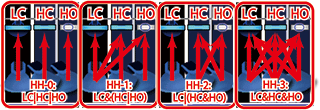
\includegraphics[scale=1.0]{Imagenes/HH_group.png}
% Ponemos Leyenda al gráfico
\caption{Grupo HH}
\label{Grupo HH}
\end{center}
\end{figure}

Obligatoria. Ya se detallara como se ha resuelto esto en el proyecto.

\subsection{HH Priority}
Aquí definimos que ha de sonar cuando tenemos \gls{Lanes} (HH-1, HH-2 o HH-3) integrados el Chip que esta en la canción o el pad que hemos tocado.
.
\subsection{FT Group}
Opción con dos modalidades que configuran la manera de trabajar en los \gls{Lanes} del tom de la izquierda, esta opción es para la gente que tiene baterias-MIDI simples con menos \gls{Pads} que los \gls{Lanes} en la canción.
\begin{itemize}
  \item FT-0 Opción en donde los \gls{Lanes} son independientes.
  \item FT-1 Los dos \gls{Lanes} anteriores se pueden tocar indistintamente.
\end{itemize}


\begin{figure}[H]
% Centramos la figura
\begin{center}
% Incluimos el gráfico y definimos el ancho y alto
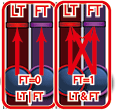
\includegraphics[scale=1.0]{Imagenes/FT_group.png}
% Ponemos Leyenda al gráfico
\caption{Grupo FT}
\label{Grupo FT}
\end{center}
\end{figure}

Obligatoria. Ya se detallara como se ha resuelto esto en el proyecto.


\subsection{FT Priority}
Aquí definimos que ha de sonar cuando tenemos \gls{Lanes} (FT-1) integrados el Chip que esta en la canción o el pad que hemos tocado.

Obligatoria.Ya se detallara como se ha resuelto esto en el proyecto.


\subsection{CY Group}
Opción con dos modalidades que configuran la manera de trabajar en los \gls{Lanes} del platillo de la derecha, esta opción es para la gente que tiene baterías-MIDI simples con menos \gls{Pads} que los \gls{Lanes} en la canción.
\begin{itemize}
  \item CY-0 Opción en donde los \gls{Lanes} son independientes.
  \item CY-1 Los dos \gls{Lanes} anteriores se pueden tocar indistintamente.
\end{itemize}

\begin{figure}[H]
% Centramos la figura
\begin{center}
% Incluimos el gráfico y definimos el ancho y alto
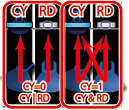
\includegraphics[scale=1.0]{Imagenes/CY_group.png}
% Ponemos Leyenda al gráfico
\caption{Grupo CY}
\label{Grupo CY}
\end{center}
\end{figure}

Obligatoria. Ya se detallara como se ha resuelto esto en el proyecto.

\subsection{CY Priority}
Aquí definimos que ha de sonar cuando tenemos \gls{Lanes} (CY-1) integrados el Chip que esta en la canción o el pad que hemos tocado.

Obligatoria. Ya se detallara como se ha resuelto esto en el proyecto.


\section{Configuraciones de uso para un futuro}

\subsection{BGA}
Opción para activar o desactivar las animaciones de Back ground.

\subsection{FillIn}
Opción para añadir efectos gráficos cuando se da a una nota en el momento justo.


\subsection{DebugInfo}
Opción que muestra información de frames per second, tiempo trasncurrido y total de la canción.


\subsection{HitSound}
Opción que activa o desactiva el sample configurado en cada lane, se suele emplear para cuando el batería ha de escuchar el resto del grupo y no lo que esta tocando él.

\subsection{SaveScore}
Opción para guardar la puntuación si es la mejor que hemos realizado hasta la fecha, esta opción es interesante ya que nos hace ver la evolución que se va teniendo a medida que se va tocando la batería, aunque seria más interesante poder tener un historial para poder analizar la mejora, y en que parte de una canción solemos fallar o estar menos sincronizados.


\subsection{D-MinCombo}
A partir de que número de combo se muestra el numero de combo actual.

\section{Configuraciones de uso que no se implementaran}

\subsection{AVI}
Para ver los videos o desactivar esta opción, se considera que se escapa al objetivo del proyecto ya que la Raspberry con tema de codecs puede tener mucha problemática, y los problemas relacionados con los DRM.

\subsection{Guitar/Bass}
El DTXMania tenia la opción de tocar la guitarra o el bajo estilo Konami, son opciones que para el batería no tienen sentido.

\subsection{StageFailed}
Es una opción que se tendría que mantener para respetar la dualidad juego/simulador si la activamos se comporta como un juego y si baja mucho la barra de vida, sale al menú de selección de canciones.

La ignoramos ya que no estamos centrando en el DTXMania como simulador/entrenador más que como juego.

\subsection{BGMSound}
El DTXMania se podía configurar de tal manera que no había música de fondo y de esta manera solo se escuchaba la batería, es una opción que no suele tener mucho sentido ya que la mayoría de baterías-MIDI tiene una salida de altavoces donde se escucha la batería en sí.



\section{Otras configuraciones}
También existía la opción de crear un archivo con unas características especiales en los directorios de las canciones para conseguir los siguientes beneficios.

Estructura de un archivo box.def de ejemplo:

\begin{Verbatim}[frame=single]
#TITLE: FROM DTX Collection
#ARTIST: FROM
#COMMENT: Dazzling floor-tom sequences.

#PREIMAGE: preimage.jpg  (or #PREMOVIE: premovie.avi)
#PREVIEW: preview.wav
#FONTCOLOR: #FFFFFF
#PERFECTRANGE: 34        (Release 068 (080427) or later)
#GREATRANGE: 67          (Release 068 (080427) or later)
#GOODRANGE: 84           (Release 068 (080427) or later)
#POORRANGE: 117          (Release 068 (080427) or later)
\end{Verbatim}

Se podía obtener varios beneficios:

\begin{itemize}
\item Tener una imagen y información para el directorio de algunas canciones.
\item Una sincronización especifica para un directorio, de esta manera era muy típico tener una carpeta con ritmos básicos para practicar.
\end{itemize}

Seria interesante en un futuro analizar estos archivos.

\chapter{Formato xa}
Anteriormente se vio que el DTXMania emplea el formato xa, se tiene que explicar que es este formato y dar una posible solución para el proyecto.
El formato .xa es un formato de sonido que usaron en BandJAM (programa japones de música, hace mucho en desuso) pero desde el inicio del DTXMania ha usado este formato hasta la actualidad.

Para ello el autor del DTXMania contacto con el autor original para usar este formato, añadió una pequeña documentación en ingles y no ha habido cambios desde entonces.

Las fuentes de este formato están disponibles en \url{http://www.dtxmania.net/wiki.cgi?page=qa_utility_e}

Más concretamente donde se indica donde se puede bajar el xadec.dll asociado a este formato
E indica:

``The original one is made by Shinichi Nakamoto (the author of BandJAM), and I (yyagi and staff) add English docmentations.''

Aquí ya indica que esta librería es para uso del formato xa, usado en GDAC2 DTXC y DTXMania.
Aunque solo hemos pasado por encima del formato del DTXMania ya hemos podido observar que es un archivo de texto, pero para dar facilidad a los músicos para que usaran este formato hay herramientas para creación de canciones en el formato DTXMania, esto sale de la idea de este proyecto.
Estas utilidades para crear canciones para facilidad de los creadores de canciones también usan este .dll.

\section{Problemas}
Como primera opción para resolver este problema, observemos que hizo el único programa que existe para entornos libres, que actualmente no se puede compilar ya que usaba librerías que actualmente están deprecated, el Digiband mencionado anteriormente dentro de su código existen zonas del código que se compilaran dependiendo de la plataforma donde estemos compilando linux o Windows, pasamos a detallar esto.

Dentro del Digiband en el archivo decodexa.C nos encontramos el siguiente código.
\begin{lstlisting}[language=C, frame=single]  
/*Oh... nothing like using a library that you have no idea how it works
 and no idea what to do with the data it gives you and the only documentation 
 you have is a example program.
 Well at least this way I was able to 'hack' it and figure out how it works by
 poking its header file.  Thank you bandjam.net for allowing public use of the 
 codec.  It's just to bad the codec has a round about usage.
*/
#ifndef LINUX
bool decodexa(char soundfile[300])
\end{lstlisting}

Por lo que se podía decodificar estos archivos si se estaba en Windows pero no en Linux.

En la documentación que se puso en aquellos tiempos para poder compilar y crear el xadec.dll se observa lo siguiente:

\begin{lstlisting}[language=C, frame=single]  

#ifndef		_XADEC_H_
#define		_XADEC_H_

/*-------------------------------------------------------------*/
#include	<windows.h>
#include	<windowsx.h>
#include	<mmsystem.h>

/*--------------------------------------------------------------*/
#define		_XAID (ULONG)(('1'<<24)|('D'<<16)|('W'<<8)|'K')
/*--------------------------------------------------------------*/
typedef struct _XASTREAMHEADER {
	UCHAR *pSrc;
	ULONG nSrcLen;
	ULONG nSrcUsed;
	UCHAR *pDst;
	ULONG nDstLen;
	ULONG nDstUsed;
} XASTREAMHEADER;

typedef struct _XAHEADER {
	ULONG id;
	ULONG nDataLen;
	ULONG nSamples;
	USHORT nSamplesPerSec;
	UCHAR nBits;
	UCHAR nChannels;
	ULONG nLoopPtr;
	SHORT befL[2];
	SHORT befR[2];
	UCHAR pad[4];
} XAHEADER;

typedef HANDLE HXASTREAM;
\end{lstlisting}

Donde el autor emplea código asociado a la plataforma Windows para definir bastantes cosas de este formato, ya que aunque se podría pensar que solo poniendo los tamaños correctos se podría compilar, también usa detalles internos del Windows para tener detalles del sonido.

Esta opción se valoro para hacer que el reproductor de DTXMania en entornos libres, funcionara indistintamente de los formatos internos del DTXMania pero tal además de los problemas citados anteriormente no queda bien integrar formatos cerrados en entornos libres.

\section{Solución aportada al proyecto}
Para dar una opción viable en entornos libres, se paso a analizar las utilidades para crear canciones con el formato DTXMania, estas utilidades obligan a tener este xadec.dll (todas las utilidades para crear .dtx están en Windows y japones) y también indican que podemos tener la utilidad xa.exe para poder transformar de .wav a .xa.

El formato DTXMania desde los inicios acepta .xa o .wav indistintamente lo que antes por consumo de memoria a la hora de reproducir la canción y por tamaño a la hora de pasarlo vía Internet se aconsejaba usar los .xa.

Para no perder todas las canciones que si que tienen un o varios .xa lo que se ha comprobado es que esta utilidad para transformar de wav a xa, también puede hacer el sentido inverso.

Se vuelve a  a tener un problema esta utilidad evidentemente esta pensada para Windows.
Lo bueno es que al ser tan simple (es una utilidad vía linea de comandos), se ha probado mediante wine y ha funcionado.

Por lo que con un pequeño script, podemos pasar de canciones DTX ``no libres'' a canciones totalmente ``libres''.


\begin{lstlisting}[language=bash, frame=single]
find . -type f -iname *.dtx -exec sh -c 'iconv -f $(file -bi "$1" |sed -e "s/.*[ ]charset=//") -t utf-8 -o converted "$1" && mv converted "$1"' -- {} \;
find . -iname '*.xa' -execdir wine ../xa122/xa.exe -d -u '{}' \;
find . -iname '*.dtx' -execdir sed -i -e 's/.xa/.wav/g' '{}' \; 
find . -iname '*.dtx' -execdir sed -i -e 's/.XA/.wav/g' '{}' \;
find . -iname '*.dtx' -execdir sed -i -e 's/\\/\//g' '{}' \;
find . -type f -iname "*.mp3" -exec bash -c 'FILE="$1"; ffmpeg -i "${FILE}"  -acodec libvorbis "${FILE%.mp3}.ogg";' _ '{}' \;
find . -iname '*.dtx' -execdir sed -i -e 's/.mp3/.ogg/g' '{}' \; 
\end{lstlisting}

Los trabajos realizados mediante este script son los siguientes:

\begin{itemize}
  \item Convertir los ficheros .dtx desde su codificación de origen a UTF-8.
  \item Usar el programa xa de tal manera que convierta los .xa a .wav, con el comando find ya coge tanto los .xa como los .XA.
  \item Transformar internamente los .dtx para que apunte a los nuevos .wav.
  \item Transformar el caracter especial de directorio de windows al de linux.
  \item Convertir los ficheros de .mp3 a .ogg, y canviar los .dtx en consecuencia.
\end{itemize}


Indicar que esto rompe un poco el espíritu del proyecto ya que esta transformación solo la podemos hacer o en un Windows o con este script en un linux x86, luego una vez transformado si que funcionaria en cualquier plataforma tanto x86 como arm.

\chapter{Formato DTXMania al completo}

Pasamos a indicar las especificaciones formales dentro del formato DTXMania, para ello vamos a la página web \url{http://dtxmania.net/wiki.cgi?page=qa_dtx_spec_e}

\section{Estructura básica}

Como ya se ha visto anteriormente la estructura básica de un archivo .dtx se compone de dos parte cabecera y objetos.

En la cabecera ira la información genérica de la canción y en la parte de los objetos toda la notación musical.


Todos los comandos se definen en lineas.
\begin{itemize}
  \item DTXMania ignora todas las lineas que no comienzan por \#
  \item DTXMania ignora las lineas que no tengan un descriptor definido.
\end{itemize}

Los comentarios dentro de los DTX son a partir del carácter ; hasta el final de la línea.

Se aconseja que no se usen a mitad de la linea ya que antiguamente un creador de dtx no lo soportaba por lo que se podía tener problemas de abrir archivos .dtx en ese creador y que hubiera problemas.

Los formatos de sonido soportados son .wav, .xa, .mp3 y .ogg, ya se ha solucionado el posible problema con los .xa y los .mp3 desde hace un tiempo ya aconseja el propio autor del DTXMania por tema de licencias usar el .ogg antes que el .mp3.

Los ficheros de imágenes soportados por el DTXMania son el .bmp, .png y .jpg.

Los ficheros de video indica que soporta tanto los .VFW (video for Windows) o AVI, recordar que no es el objetivo principal de este proyecto el tratar ficheros de video.

Se tiene que detallar todos los comandos documentados para nuestro reproductor de .dtx, se separan en tres grandes bloques: a implementar, detallar para un futuro o  no implementar por salir de la idea del proyecto.

\section{Cabecera}

Cuando en la documentación se indica zz lo que se define es decimal más letras en mayúsculas por lo que se tiene las siguientes posibilidades (01-ZZ) 

\section{Comandos en cabecera a implementar}

\subsubsection{\#TITLE}
\#TITLE <song title>

\subsubsection{\#PANEL}
\#PANEL <comments on playing screen>

Es un comentario que se vera con un scroll mientras se juega la canción, se suele usar en las canciones para entrenamiento indicar como se tienen que tocar.

Si no existe este parametro se usa \#TITLE

\subsubsection{\#DLEVEL}
\#DLEVEL <level value>

Dificultad de la canción en batería.

\subsubsection{\#BPM}
\#BPM <the value of BPM>

El valor del BPM al inicio de la canción, se puede usar decimales.
\subsubsection{\#BPMzz}
\#BPMzz <the value of BPM>

Posible valor de BPM, durante la canción se modificara mediante el canal 08 apuntando al valor de la ``nota de cambio'' zz.¡

\subsubsection{\#BASEBPM}
\#BASEBPM <the value of BASEBPM>

El valor base de las BPM al cual se añadirán o restaran valores para modificar los BPM durante la canción.


\subsubsection{\#PREIMAGE}
\#PREIMAGE <preview image filename>

Imagen que se mostrara en la pantalla de selección.

\subsubsection{\#WAVzz}
\#WAVzz (WAV, MP3, XA or OGG) filename>


Define el sonido del banco zz. Para que nuestro reproductor del DTXMania sea lo más libre posible recomendamos solamente WAV o OGG.

Cada canal de batería tiene dos-polifonias posibles.


\section{Comandos en cabecera para un futuro}

Define el nombre de la canción.
\subsubsection{\#ARTIST}
\#ARTIST <artist name>

Define el nombre del artista.

\subsubsection{\#GENRE}
\#GENRE <genre name>

Define el genero de la canción.

\subsubsection{\#COMMENT}
\#COMMENT <comments of yours>

Pone un comentario.

\subsubsection{\#STAGEFILE}
\#STAGEFILE <now loading image filename>
Se puede usar archivos en BMP, JPEG o PNG. Y se mostraran en el momento de cargar la canción.


\subsubsection{\#BACKGROUND}
\#BACKGROUND <wallpaper filename>

Wallpaper que se usara mientras se reproduce la canción.


\subsubsection{\#WALL}

\#WALL <wallpaper filename>

Lo mismo que background.

\subsubsection{\#PREVIEW}
\#PREVIEW <preview sound filename>

La música que sonara como muestra en el menú de selección.


\subsubsection{\#BMP}
\#BMP <BGA image file>

Pone la imagen de fondo inicial.


\subsubsection{\#SOUND\_NOWLOADING}
\#SOUND\_NOWLOADING <nowloading sound filename>

Define el sonido que se escuchara mientras estamos en la pantalla de ``now loading''.


\subsubsection{\#SOUND\_STAGEFAILED}
\#SOUND\_STAGEFAILED <stage failed sound filename>

Define el sonido que se escuchara mientras estamos en la pantalla de ``stage failed''.

\subsubsection{\#SOUND\_FULLCOMBO}
\#SOUND\_FULLCOMBO <full combo sound filename> 

Define el sonido que sonara si hacemos un full combo.

\subsubsection{\#RESULTIMAGE}
\#RESULTIMAGE <result screen image filename>

Imagen que se mostrara al final de la canción.
Si no esta definido se usara \#PREIMAGE.
También se puede usar \#RESULTIMAGE\_xx que puede cambiar la imagen resultante dependiendo de que rango se obtenga al tocar la canción.

\begin{Verbatim}[frame=single]
#PREIMAGE resimage0.jpg
#RESULTIMAGE_A resimage1.jpg
#RESULTIMAGE_D resimage2.jpg

;Si tu rango es...
; -SS, S or A: resimage1.jpg 
; -B, C or D: resimage2.jpg 
; -E: resimage0.jpg 

\end{Verbatim}


\subsubsection{\#RESULTIMAGE\_xx}
\#RESULTIMAGE\_xx <result screen image filename>

Mirar \#RESULTIMAGE

\subsubsection{\#RESULTSOUND}
\#RESULTSOUND <result screen sound filename>

Sonido que se usara en la pantalla de resultados.


\subsubsection{\#RESULTSOUND\_xx}
\#RESULTSOUND\_xx <result screen sound filename>

Sonido que se usara dependiendo del rango obtenido, para el uso mirar la sección RESULTIMAGE.


\subsubsection{\#VOLUMEzz}
\#VOLUMEzz <volume percentage>

Ajusta el volumen en el banco de sonido zz.

\subsubsection{\#PANzz}
\#PANzz <panning position parameter>

Ajusta el posicionamiento del stereo en el banco de sonido zz, el uso va de -100 a 100.


\subsubsection{\#SIZEzz}
\#SIZEzz <chip display size percentage>

Sirve para definir el tamaño de las notas en el canal zz. Puede ser útil para mostrar visualmente que las notas aunque esten en el mismo lane, tienen volumen distinto o realmente se tendria que tocar con varios instrumentos.

\subsubsection{\#BMPzz}
\#BMPzz <image filename>

Define la imagen que se empleara para el chip del canal zz. 




\section{Comandos en cabecera que no se implementaran}

\subsubsection{\#GLEVEL}
\#GLEVEL <level value>

Dificultad de la canción en guitarra.

\subsubsection{\#BLEVEL}
\#GLEVEL <level value>

Dificultad de la canción en bajo.

\subsubsection{\#PREMOVIE}
\#PREMOVIE <preview movie filename>

Video que se pondría en el menú de selección. No es el objetivo del proyecto manejar ficheros de video.

\subsubsection{\#HIDDENLEVEL ON}
\#HIDDENLEVEL ON

Pone la dificultad como ??. 


\subsubsection{\#BACKGROUND\_GD}
\#BACKGROUND\_GD <wallpaper filename>

Wallpaper que se usara en el modo guitarra.


\subsubsection{\#RESULTMOVIE}
\#RESULTMOVIE <result movie filename>

La película que se vera cuando se acaba la canción. 

\subsubsection{\#RESULTMOVIE\_xx}
\#RESULTMOVIE\_xx <result movie filename>

La película que se vera dependiendo del rango.


\subsubsection{\#MIDINOTE}
\#MIDINOTE <ON|OFF>

Se puede usar para que salga en el canal 10 de MIDI-OUT. Lo que se esta tocando. No se implementara ya que las dos principales baterías-MIDI que se han tomado por defecto en este proyecto ya tienen formas de tener MIDI-OUT.

\section{Objetos}
Descripción de los objetos


\subsubsection{\#nnncc object list}
Se define la notación de la siguiente manera:

\begin{itemize}
  \item nnn Compas número nnn en decimales (000-999)
  \item cc El canal en hexadecimal (01-FF)
  \item object list - lista de objetos
\end{itemize}

\subsubsection{Formato de lista de objetos}
Se define la lista de objetos como donde y que \gls{Chips} están una barra y un canal distribuidos uniformemente en la barra.
Cada objeto esta definido como una expresión de 2 dígitos en 36-decimales (números y letras) por lo que cada objeto va entre (00-ZZ).

El objeto 00 esta definido como el silencio, y los demás objetos tendrán su banco de sonido asociado mediante el comando en cabecera de \#WAVzz

Para entender esto lo mostraremos con un ejemplo, definiremos la siguiente partitura:


\begin{figure}[H]
% Centramos la figura
\begin{center}
% Incluimos el gráfico y definimos el ancho y alto
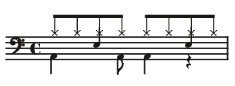
\includegraphics[scale=5.0]{Imagenes/explicacion-lista-objetos.jpg}
% Ponemos Leyenda al gráfico
\caption{Explicación lista objetos}
\label{Explicación lista objetos}
\end{center}
\end{figure}


\begin{Verbatim}[frame=single]
  #WAV01 hihat.wav
  #WAV02 snare.wav
  #WAV03 bass.wav

  #00111 0101010101010101
  #00112 00020002
  #00113 0300000303000000
\end{Verbatim}

Vamos a separar explicar cada línea.

\begin{Verbatim}[frame=single]
"#00111 0101010101010101" -> "#00111 01 01 01 01 01 01 01 01"
\end{Verbatim}

Significa que en el primer compás (001), en el canal (11) que es el del hihat ponemos ocho objetos distribuidos uniformemente de tipo (01) que también se ha definido como el sonido hihat.wav. 

De la misma manera:

\begin{Verbatim}[frame=single]
"#00112 00020002" -> "#00112 00 02 00 02"
\end{Verbatim}

Significa que en el primer compas (001), en el canal (12) definido como el snare ponemos cuatro objetos distribuidos uniformemente (00 02 00 02).


\begin{Verbatim}[frame=single]
"#00113 0300000303000000" -> "#00113 03 00 00 03 03 00 00 00"
\end{Verbatim}

En el primer compás (001) en el canal (13) bombo, ponemos la siguiente lista de objetos (03 00 00 03 03 00 00 00).

Se puede insertar los caracteres \_\_ que no afectan a la semántica pero pueden ayudar a la lectura humana de la partitura.

\begin{Verbatim}[frame=single]
  #00111 01010101_01010101     / or 01010101_01010101
  #00112 0002_____0002         / or 00__02___00__02__
  #00113 03000003_03000000     / or 03000003_03000000
\end{Verbatim}

Si existe varias lista sobre el mismo tiempo y el mismo canal se mezclaran.

Ejemplo:


\begin{figure}[H]
% Centramos la figura
\begin{center}
% Incluimos el gráfico y definimos el ancho y alto
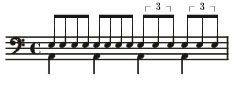
\includegraphics[scale=5.0]{Imagenes/particion_varias_listas.jpg}
% Ponemos Leyenda al gráfico
\caption{Explicación varias lista objetos }
\label{Explicación varias lista objetos}
\end{center}
\end{figure}

\begin{Verbatim}[frame=single]
  #00112 02020202_02020202_00000000_00000000   -> primera parte (dieciséis notas)
  #00112 000000___000000___020202___020202     -> siguiente parte (tripletas)
  #00113 03_______03_______03_______03
\end{Verbatim}

No se permitirá en este proyecto la mezcla en el compás, lane y canal ya que no esta definido que hacer si se mezclan varias notas, y no es una opción muy usada en los .dtx.

\section{Canales definidos por el DTXMania}

Se pasa a definir los canales del DTXMania, para ello se usara la misma manera de separarlos en tres tipos: canales a implementar, canales para un futuro y canales que se escapan al objetivo del proyecto.


\section{Canales a implementar}

\subsection{01 - BGM Back chorus}
Canal empleado para los coros este canal es polifónico, se podrían emplear los canales de 61 al 92 pero esas son monofónicas.

\subsection{03 - BPM}
Se cambiara el número de beats por minuto, esta especificado en hexadecimales (01-FF)
Pensar que este valor se añade a la BASEBPM

\begin{Verbatim}[frame=single]
  #BPM 220
  #BASEBPM 200

  #03103 0042
\end{Verbatim}

Al principio, BPM=220.
A partir del compás 31, 03 mitad de la barra se cambiar los BPM a 266 
(42 hexadecimal = 66 + 200)

Esto es lo indicado en la documentación se ha probado y lo que realmente se tiene que hacer es, si esta en la primera nota del compás cambiar los BPM del compás actual y si no cambiar los BPM para el siguiente compás.


\subsection{08 - Extended tempo(BPM)}
En el canal 03 se ha definido el tempo como un objeto directo, que se tenia que sumar a un valor base, aquí se define el tempo con los valores zz.

Se suele usar el canal 03 para BPM enteros y para BPM reales se usa este canal.

\begin{Verbatim}[frame=single]
#BPM 123.45
#BPM01 234.56
#00303 00007000
#00603 00010000
\end{Verbatim} 

BPM=123.45 Desde el principio de la canción hasta el tercer compás y segundo beat.

BPM=112.00 desde el tercer tiempo, tercer beat. 

(112 decimals = 70 hexadecimals)

BPM=234.56 desde el sexto tiempo segundo beat hasta el final de la canción.

En caso de BASEBPM=0


Esto es lo indicado en la documentación, se ha probado y lo que realmente se tiene que hacer es, si esta en la primera nota del compás cambiar los BPM del compás actual y si no cambiar los BPM para el siguiente compás.


\subsection{11-1A - Notas de la batería}
Canales visuales donde se pondrán los \gls{Chips} que veremos, los canales y los \gls{Lanes} están relacionados de la siguiente manera:


\begin{Verbatim}[frame=single]
11 = HiHatClose
12 = Snare
13 = BassDrum
14 = HighTom
15 = LowTom
16 = Cymbal
17 = FloorTom
18 = HiHatOpen
19 = RideCymbal
1A = LeftCymbal (DTXMania Release 064b061229 or later)
1F = Fill sound drums
\end{Verbatim} 

No se implementara el canal 1F e indicar también que se tiene que implementar los canales 1B y 1C para tener compatibilidad con las canciones del DTXManiaHD y del gitadora, esto no esta en ninguna documentación del DTXManiaHD o del gitadora se ha tenido que obtener vía ingeniería inversa..

El canal 1B es para el pie izquierdo para el doble bombo y el 1C también para el pie izquierdo para el sonido del hihat.

\subsection{61-62- Sonidos en autoplay}
Canales que están definidos en autoplay, se usan para poner sonidos adicionales.

\section{Canales a implementar en un futuro}

\subsection{02 - BAR length}
Este canal controla la longitud de la barra.
El valor puede ser decimal o flotante, pensar que se cambia la longitud de toda la barra.


 \begin{itemize}
   \item Valor de 1 es el de defecto es equivalente a un ritmo 4/4.
   \item 0.75 significaría un ritmo 3/4
   \item 1.0625 significaría un ritmo 17/16.
 \end{itemize}

\begin{Verbatim}[frame=single]
  #01902 0.75
  #01911 010101
  #01912 010101010101010101
\end{Verbatim}

Este valor se mantiene, hasta que haya otro cambio o final de la canción.

\begin{figure}[H]
% Centramos la figura
\begin{center}
% Incluimos el gráfico y definimos el ancho y alto
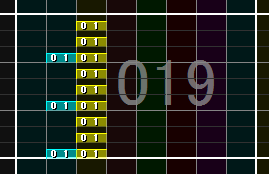
\includegraphics[scale=1.0]{Imagenes/canal_reducido.png}
% Ponemos Leyenda al gráfico
\caption{Explicación barra reducida}
\label{Explicación barra reducida}
\end{center}
\end{figure}


\subsection{04 - BGA}
Canal donde se define el BackGround Animation.

\subsection{07 - BGA/ 2 capa}
Muy parecido al canal 04 pero con dos capas.

\subsection{31-3A - Drums invible object}
Este canal se emplea para que cuando se falle el chip de un canal de batería tener otro sonido definido, tienen una relación directa con los canales de la batería.

\begin{Verbatim}[frame=single]
31 = HiHatClose
32 = Snare
33 = BassDrum
34 = HighTom
35 = LowTom
36 = Cymbal
37 = FloorTom
38 = HiHatOpen
39 = RideCymbal
3A = LeftCymbal (DTXMania Release 059 or later)
\end{Verbatim}

\subsection{50 - BAR line}
Aunque los tiempos son manejados internamente por el DTXMania se puede hacer que se vean los BAR line en la canción explícitamente.

\subsection{51 - Beat Line}
Aunque los tiempos son manejados internamente por el DTXMania se puede hacer que se vean los beats en la canción explícitamente.

\subsection{53 - Fill in}
Define una zona 01 al inicio 02 al final, para escuchar el sonido de ánimos cuando se comienza un combo o se acaba.

\subsection{55-59,60 - BGA / capas}
Lo mismo que el canal 04, pero más capas para poder definir varios fondos.


\subsection{63-69, 70-79,80-89,90-92 - Sonidos en autoplay}
Canales que están definidos en autoplay, se usan para poner sonidos adicionales.

\subsection{B1-B9, BC No-chip default sound}
Parecido a los canales 31-3A
Aquí se define que suena si no hay chip, pero este canal se puede ir definiendo hasta el final de la canción. por lo que se puede ir modificando estos sonidos.

\begin{Verbatim}[frame=single]
B1 = HiHatClose
B2 = Snare
B3 = BassDrum
B4 = HighTom
B5 = LowTom
B6 = Cymbal
B7 = FloorTom
B8 = HiHatOpen
B9 = RideCymbal
BC = LeftCymbal (DTXMania Release 059 or later. Note: it's NOT BA!)
\end{Verbatim}

\subsection{C1 [BEAT-line shifting]}
La linea de BEAT comenzara en ese BAR donde se haya definido en este canal C1 con el valor 02, no afecta al siguiente BEAT.

\subsection{C2 [hide BEAT/BAR lines]}
Se puede ocultar los chips para ello hay que poner el valor 02 en este canal. Para volverlos a mostrar hay que poner el valor 01.

\subsection{C4, C7, D5-D9, E0 [Swapping BGA bitmap] }
Canales para ir cambiando la imagen de fondo.


\section{Canales que no se implementaran}

\subsection{00}
Tempo esta obsoleto.

\subsection{05 - Extend object}
No implementado en el DTXMania.

\subsection{06 - Cambiar la animación de MISS}
No implementado en el DTXMania.

\subsection{09-10 - Reservados por BMS}
Reservado para otros juegos musicales.

\subsection{20-29 y 2F- Notas de la guitarra}
Estos canales son para la guitarra

\subsection{30 - flow-speed drums}
No estaba soportado por el DTXMania por lo que nosotros tampoco lo implementaremos.

\subsection{40 - Reservado por BMS}
Reservado para otros juegos musicales.

\subsection{41-46 Invisible object for the 2nd player}
No implementado en DTXMania.

\subsection{47-49 - Reservado por BMS}
Reservado para otros juegos musicales.

\subsection{52 - MIDI drum chorus}
Para enviar la nota a través de canal MIDI-10.

\subsection{54 - Playback movie}
Para ver una película especificada en \#AVIzz.


\subsection{93-99 - Reservados}
Reservados.

\subsection{A0-A7 - Bass notes}
Canales para el bajo, no se tendrá en cuenta para este proyecto

\subsection{A8 - Wailing (Bass)}
Canal para el bajo, no se tendrá en cuenta para este proyecto

\subsection{AF - Wailing sound (Bass)}
Canal para el bajo, no se tendrá en cuenta para este proyecto

\subsection{BA - No chip default sound (guitar)}
Canal para la guitarra, no se tendrá en cuenta para este proyecto

\subsection{BB - No chip default sound (bass)}
Canal para el bajo, no se tendrá en cuenta para este proyecto.


\section{Comentarios sobre el proyecto}
Ahora que ya se tiene el concepto de que es  un .dtx y debido a todos los posibles canales se  dejara en la salida del terminal todos los objetos que no se han implementado, tanto objetos o canales de esta manera si un .dtx no suena correctamente se podrá observar que características de los .dtx se están intentando emplear y no están implementadas.

También se tendrá que mirar el formato .dtx usado en las canciones del DTXmaniahd y gitadora, ya que se ha ido ampliando el formato, y no se ha ido ampliando la documentación en ingles, se ha implementado dos canales que no estaban en la documentación original.

\chapter{Especificaciones generales de diseño}
\section{Consideraciones generales a python3}

Ahora ya se tiene una idea más clara de todo lo que se tendrá que implementar en el proyecto, por lo que se pueden evaluar las posibles librerías de python a usar.

Primero se detallaran unas consideraciones generales a todo el código python que se escribirá para el proyecto.

El texto empleado en las pantallas estará en ingles, para un mayor acceso a la comunidad de baterías a nivel mundial.

Se ha escogido python y la versión python3 más concretamente para este proyecto, ya que es un lenguaje interpretado y gracias a ello, sin tener que recompilar se tendrá el proyecto tanto en las plataformas x86 como en las plataformas ARM (se tendrá para otras plataformas pero no estará probado).

Ya que python es un lenguaje que tiene muy buen control sobres listas y diccionarios se integrará este control en el proyecto, principalmente para obtener tres objetivos al mismo tiempo:

 \begin{itemize}
   \item Al usar los iterators en las listas para recorrer estas el código es más rápido.
   \item Al usar las keys de los diccionarios para buscar la información de estos, el tiempo es optimo.
   \item Lectura y mantenimiento del código.
 \end{itemize}

  Para mantener este tercer punto de manera integrada en el proyecto, las variables de tipo lista siempre comenzaran sus nombres como:

\begin{lstlisting}
    list_
\end{lstlisting}
  
  
Y las variables de tipo diccionario empezaran por:

\begin{lstlisting}
    dict_
\end{lstlisting}
 
 Se emplearan listas cuando el orden importe, y diccionarios cuando no.
 Para los diccionarios la llave de estos normalmente sera el nombre de la lane asociada de esta manera estará optimizado para su uso, ya que la gran mayoría de búsquedas que se harán en el código se buscara por lane.


Se escogerá la versión de python 3.4 debido a que es la soportada en las principales distribuciones en la raspberry, por lo que no se tendrá que usar ninguna instrucción para versiones superiores.




\subsection{Posibles librerías gráficas y de sonido: pygame / tkinter / Qt5}

Este proyecto tiene una gran carga tanto en sonido como en gráficos, no por complejidad de estos si no más bien debido al tratamiento en tiempo real de estos.

Recordar que en música se indica que un instrumento musical se puede tocar si tiene menos de diez milisegundos de retardo entre la acción y que suene.


En python3 hay tres grandes librerías para tratar los gráficos de una manera rápida y cómoda.

Pygame, librerías especializadas en creación de videojuegos 2d.

PyQT5, wrapper a las librerias Qt5, con toda su documentación y su control multiplataforma.

TkInter, la libreria ``casi'' standard de python.


Tkinter tiene el problemas que para hacer las animaciones se debería programar todo el control de tiempo sobre ellas, al mismo tiempo que se esta teniendo el control del sonido, por lo que se deshecha por demasiado simple.

PyGame tiene la ventaja que al estar pensada para videojuegos tiene un buen control sobre los tiempos, pero tiene dos grandes inconvenientes para este proyecto, el primero y más sencillo es que debido a su bajo nivel, el programador tiene que empezar casi de cero para crear toda una interfaz gráfica, el segundo punto es que no tiene una fácil escalabilidad si la plataforma soporta OpenGL.

PyQT5, tiene una muy buena documentación y escala bien con el OpenGL, por lo que se puede programar de tal manera que si las librerías Qt5 detectan que la plataforma soporta OpenGL automáticamente acelerar toda la interfaz gráfica.

Una gran ventaja de las librerías Qt5 es que en su integración con Python, las llamadas para animar gráficos o reproducir sonidos no bloquean el interprete de python, se puede entender que son llamadas en paralelo, aunque que por el GIL (Global Interpreter Lock) de python esto no es del todo cierto.

 
Aunque se podría usar unas librerías gráficas para los menús y otras librerías gráficas para la parte mientras se esta reproduciendo la canción en sí, es mejor evitarlo para no tener problemas de que librerías recogen los eventos de teclado, ratón, foco de la pantalla.

Para el proyecto se ha decidido usar las librerías Qt5.
 

\subsection{Configuraciones en disco duro: configparser}
Como en este proyecto no hay necesidad de usar unas configuraciones muy complicadas se ha optado por usar la librería de python configparser, para cargarlas y guardarlas en el disco duro. Ya que són las librerias aconsejadas por la comunidad de python para estos casos.


\subsection{MIDI: pygame / Cython y rtmidi2}
Observando las librerías disponibles para tratar el MIDI en python3 se observo que existen solamente dos grandes librerias en python, pygame y rtmidi

El problema con pygame es el comentado anteriormente de usar unas librerias para los menús y otras para la parte de la reproducción de la canción en sí.

Las librerias rtmidi2 es una librería basada en Cython (que es la manera que tiene python de llamar a posibles librerías en C) el detalle es que esta librería es muy poco usada por lo que habitualmente se tendrá que descargar, tanto la librería en C, como compilar para el python instalado en el sistema las librerias Cython y rtmidi2.
 
La gran ventaja de usar este estilo de librerías es que al estar a tan bajo nivel son muy rápidas y se consume poca memoria ya que casi no hay aumento de memoria comparado con las librerías en C.

 
Viendo las posibilidades se ha optado por rtmidi2 que mediante Cython, se podrán usar los comandos de la librería rtmidi de C dentro de python.


\section{Gráficos en qt5}

Una de las grandes ventajas de emplear Qt5 como la base para los gráficos es que en todos los menús, se tiene separado la parte gráfica de la parte funcional, para ello se tienen los archivos .ui, que mediante el creador que da Qt, se puede crear de manera gráfica todos los elementos estilo ventanas, botones , imágenes, y luego mediante un sistema de eventos y señales les podremos dotar una cierta funcionalidad.

Los ficheros .ui estarán en una carpeta llamada ui, dentro del código fuente.

Cada vez que se quiera hacer un cambio gráfico en el proyecto se tendrá que generar los .py asociados a estos .ui mediante pyuic5, de esta manera en entornos de poco recursos se optimizara ya que estos python ya estarán generados, como buena practica de programación se aconseja no tocar estos ficheros generados por Qt, por lo que se tendrá que tener clases que se deriven de estos python generados.

\section{Animaciones en qt5}
Qt5 tiene un motor para hacer sus animaciones, dentro de los widgets gráficos, estan animaciones tanto pueden ser animaciones secuenciales como paralelas entre ellas.


Recordar que el lenguaje python es interpretado y tiene un garbaje collector por lo que tendremos que tener especial cuidado en no dejar de apuntar a los objetos a los que todavía tenemos que hacer referencia, aunque sea de las librerías de Qt, ya que si el garbage collector de python elimina esos objetos se podrán observar fallos gráficos.

El mismo Qt5 indica que sus timers y animaciones son aproximadas, en el aspecto que depende de la CPU su buen funcionamiento, siempre entendiendo que el refresco gráfico tiene que tener la CPU libre, para ello el mismo QT indica que lo mejor es dejar que sea su maquina de estados la encargada de actualizar todos los elementos gráficos, si se han de animar estos elementos gŕaficos Qt da la manera de ir agrupandolos en animaciones tanto paralelas como secuenciales, y la maquina de estados de Qt, animara de una manera o de otra dependiendo de si están en pantalla estos elementos o no.

Como python3 tiene el GIL, Global Interpreter Lock, se entiende que aunque hay llamadas a otras librerías que si que podrían estar ejecutándose en paralelo, no es del todo así, si no que para evitar fallos de concurrencia solo hay 1 thread vivo al mismo tiempo y solo se emplea una cpu. Si queremos tener un python realmente paralelo se debería cambiar de interprete y no usar el interprete por defecto.

En referencia a los timers de Qt5 en la documentacion de Qt indican que estos tiempos no son exactos y que su exactitud depende de la plataforma y como se hayan compilado las librerias Qt, para que se pinte la pantalla se tiene que parar el interprete de python y que este deje la CPU cierto tiempo libre.

Esto puede derivar que en el algunas canciones con muchas notas y mucha velocidad, dependiendo de la cpu se pueden observar pequeñas diferencias visuales entre notas. A nivel de sonido y de comprobación de sincronización esto no afecta ya que esta lógica se hará mediante python por lo que al tener más prioridad el tiempo sera correcto.

Ahora entendiendo esto se puede plantear la animación de una canción de cuatro maneras distintas:

\subsection{Ningún timer, una gran animación}

Una posible implementación, de una canción y dada una velocidad de sincronización en concreto, es pensar en analizar la canción y crear todas las notas visuales en su lane correspondiente y en su tiempo asignado creando una animación para cada nota y que cada nota llegue al punto cero en el momento que debería ser tocada, evidentemente esto tiene el gran inconveniente de que tenemos que tener todos estos elementos gráficos en memoria aunque no estén en pantalla.

Ya que no tiene que tener la canción durante toda su duración el mismo tempo, esto junto a que se entiende como tiempo de sincronización el tiempo que tarda una nota en recorrer la pantalla visible, complica el colocar las notas en su tiempo correspondiente, ya que no todos los compases tienen la misma longitud (Dependiendo que en la canción haya cambios de tempo).

Esto en la raspberry al tener una cpu lenta, se observo que no era viable. 

\subsection{Todas las notas con su timer}

Otra posible implementación es hacer que cada nota tuviera un timer asociado de cuando debería aparecer en pantalla, de esta manera una vez creado todos los timers, el reproductor solo tendría que crear una animación para esa nota, cuando el timer se disparase.

El problema de esta implementación es que los timers no son lo suficientemente precisos, ya que aunque se puede indicar una precisión menor a  milisegundos cuando se han de disparar se nota que es una aproximación, esto sobretodo se observa en la raspberry ya que en notas dobles, que deberían sonar al mismo tiempo pero visualmente se observaban como notas separadas.


\subsection{Un timer para el siguiente compás}

Como se han comprobado con los dos casos anteriores, tener mucha información gráfica que no estamos viendo o tener muchos timers nos puede llevar a tener retardos tanto gráficos como a nivel sonoro.

Para ello se va a reducir en lo posible estos dos elementos.

Entendiendo las animaciones como bloques se puede juntar como una animación para cada compás, creando un timer para el siguiente compás, se puede entender la reproducción como animar el compás, y esperar a este timer del siguiente compás.

El problema de esta implementación es que aunque solo tengamos un timer este va acumulando retrasos en tiempo de ejecución, y eran distinguibles en una canción un poco larga ya en un ordenador en la plataforma x86 por lo que no merece la pena comentar los retrasos que se producían al probar el código en una raspberry.

\subsection{Un timer único para el control del tiempo}
Viendo que los timers proporcionados por Qt, no tienen los requerimientos de tiempo real, que si que se tienen en este proyecto, se van a implementar las animaciones y el control del tiempo usando un solo timer que sera el control de tiempo, de esta manera si que se puede saber cuando tiempo llevamos reproduciendo la canción.

Por tanto se pasa a tener un programa que en muchas partes de su código dependerá del tiempo actual que llevamos reproduciendo.

Se codificara una lista de compases por analizar, un compás analizandose en el momento actual, y una lista de chips separadas en lanes que se están animando o se ha de reproducir sin lane visual.

Por tanto se crearan los chips visuales lo más cercano posible al momento que se han de comenzar a ver.

Comentar que siempre se tratara con dos tiempos, el tiempo según el .dtx original y el tiempo donde realmente tiene sonar la nota, que sera el tiempo original más el tiempo de sincronización.
Una vez realizado un análisis del .dtx, se obtiene todas las notas en sus compases y se calcula el tiempo en el que debería sonar cada 
nota, y los tiempos de inicio de estos compases. 
Por tanto el bucle principal a la hora de reproducir, es comprobar el tiempo que llevamos de canción reproducida, si hemos alcanzado el tiempo del primer compás de la lista de compases analizar, quitar este compás y pasar a estar analizando este.
En el compás que se esta analizando tiene notas con los tiempos originales en el .dtx, cuando se llega al tiempo de una nota, se tiene que pasar esta nota a su lane correspondiente aumentado el tiempo correspondiente con el tiempo de sincronización.
 

Gracias a esta implementación se tiene solamente como memoria gráfica lo que tiene que estar en pantalla o que en breve tiene que desaparecer, recordar que sera el garbage collector el encargado de liberar esta memoria, lo que si que hay que indicar es que tenemos la cpu muy activa para tener un control de sonido muy preciso y cuando se ha acabo de comprobar las tareas de sonido y de control del reproductor se puede hacer la pausa para que el qt, pinte la pantalla.


\section{Sonidos en qt5}
Qt5, ya da la facilidad de reproducir sonidos, pero se tendrá que tener en cuenta si son .ogg o .wav ya que Qt5, no los trata igual, ya que uno tiene que descomprimir el archivo y reproducirlo mientras que en el otro solo tiene que reproducirlo.

Para un mejor funcionamiento del programa todos los sonidos los pondremos en un banco de memoria, de esta manera una vez ya comenzada la reproducción del .dtx solo tener que reproducir el sonido sin tener que hacer la carga a memoria.

Por definición de los sonidos en los dtx, los lanes visuales tendrán sonidos asociados estilo .wav, ya que los sonidos de la batería tienen que tener la menor latencia posible.
Lo que no se puede asegurar de los sonidos asociados a los lanes no visuales, ya que se suelen poner los .ogg en canciones donde hay más música aparte de la batería, pero en las canciones de practica se suele poner los sonidos de un metrónomo con el formato .wav.

\chapter{pyDTX}
\section{Ideas generales}
Ahora que se esta definido el lenguaje a usar, las librerías que se emplearan y el formato .dtx se detallaran las ideas generales, para efectuar el proyecto.
\section{Pantalla principal}
Se trabaja con un Main Aplication dentro de Qt5, se pondrá un MainWindow ya que usaremos entorno gráfico, en este MainWindow se creara un stackedwidget, dentro del cual se tendra unos widgets independientes, de esta manera se aumenta el tiempo inicial pero luego como ya están todos los menús creados ahorramos en tiempo de computación. Como todos los widgets son bastante independientes seria muy fácil coger este código y modificarlo para otros proyectos de estilo musical, o modificar los gráficos manteniendo la estructura y lógica de python.

Dentro de este stackwidget se crearan los siguientes widgets:

 \begin{itemize}
   \item Widget Inicial
   \item Widget para configurar bateria-MIDI
   \item Widget para configurar pyDTX
   \item Widget Pantalla Navegación
   \item Widget Reproducción
 \end{itemize}


 
\section{Pantalla Inicial}
Para la pantalla incial se empleara un widget muy básico donde se pondrán cuatro botones centrados, y estos botones activaran el widget correspondiente de esta manera podemos cambiar de widgets.


Qt5 se encargara automáticamente de que solo el widget actual reciba los eventos de teclado y ratón.

El widget de la pantalla inicial tendrá una imagen de fondo dependiendo de la configuración del pydtx, aquí decir que se hará mediante .css ya que es lo más independiente del sistema y es lo que aconseja Qt5 actualmente.

\begin{figure}[H]
% Centramos la figura
\begin{center}
% Incluimos el gráfico y definimos el ancho y alto
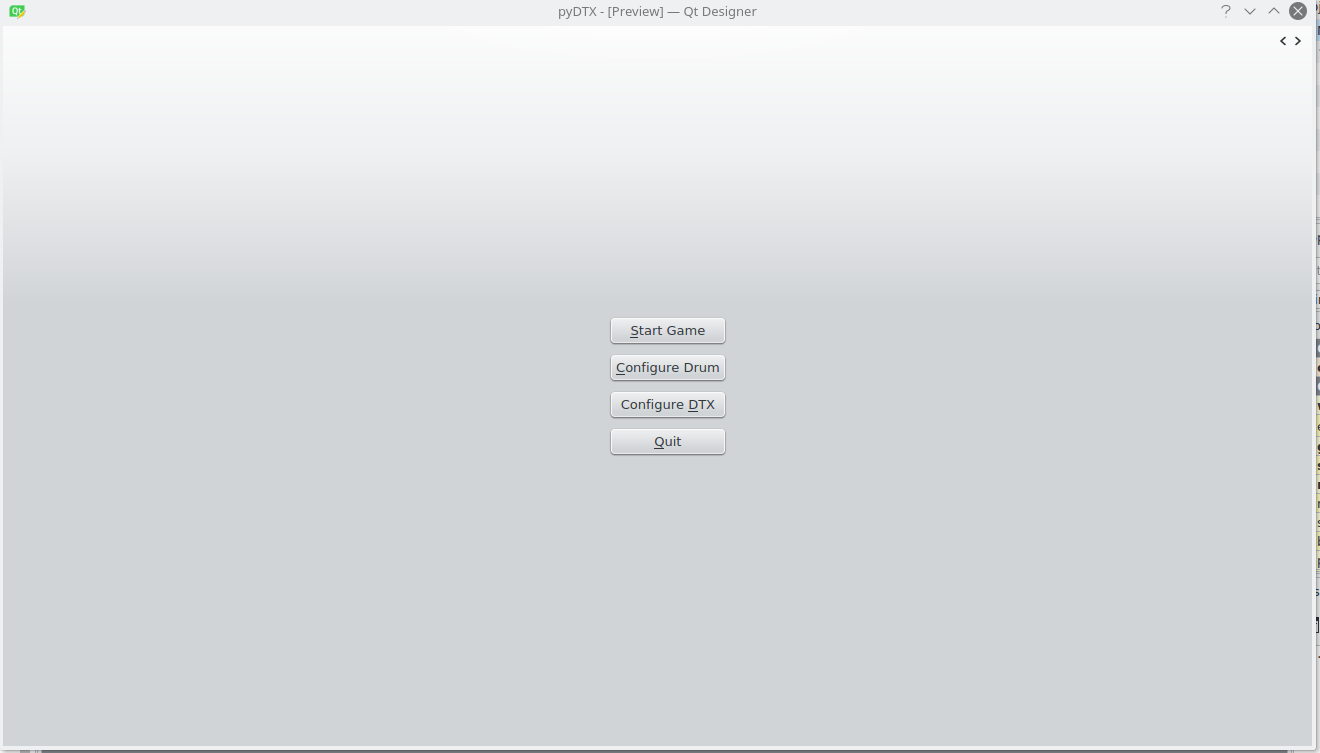
\includegraphics[scale=0.4]{Imagenes/Main_window.png}
% Ponemos Leyenda al gráfico
\caption{Pantalla Inicial}
\label{Pantalla Inicial}
\end{center}
\end{figure}


\section{Pantalla configuración batería-MIDI}
El widget que se usara para configurar la batería-MIDI tiene que poder dejar al usuario definir las posibles teclas, para cada lane visual de este pyDTX.

Como pantalla de configuración se tiene que leer el fichero de configuración, poner los elementos gráficos en concordancia y un posible de botón para guardar para que todos estos valores gráficos transformarlos en un fichero de configuración.

Además se podrá definir los lanes que configuraremos en Auto para que el mismo pyDTX, haga sonar todos los chips asociados a este lane pero continúen siendo visuales.

En esta pantalla ya hay dos cosas relacionadas con la batería-MIDI, la primera un botón para poder ver cuantos instrumentos-MIDI esta viendo el sistema operativo y de esta manera poder configurar el que queremos usar para tocar los .dtx.

Para que sea más cómodo para el usuario se pondrá un botón, para poder tocar la batería-MIDI y que en la pantalla se pueda ver que nota asociada esta emitiendo la bateria-MIDI. De esta manera el usuario podrá configurar los lanes visuales con los eventos que emite su batería-MIDI.

\begin{figure}[H]
% Centramos la figura
\begin{center}
% Incluimos el gráfico y definimos el ancho y alto
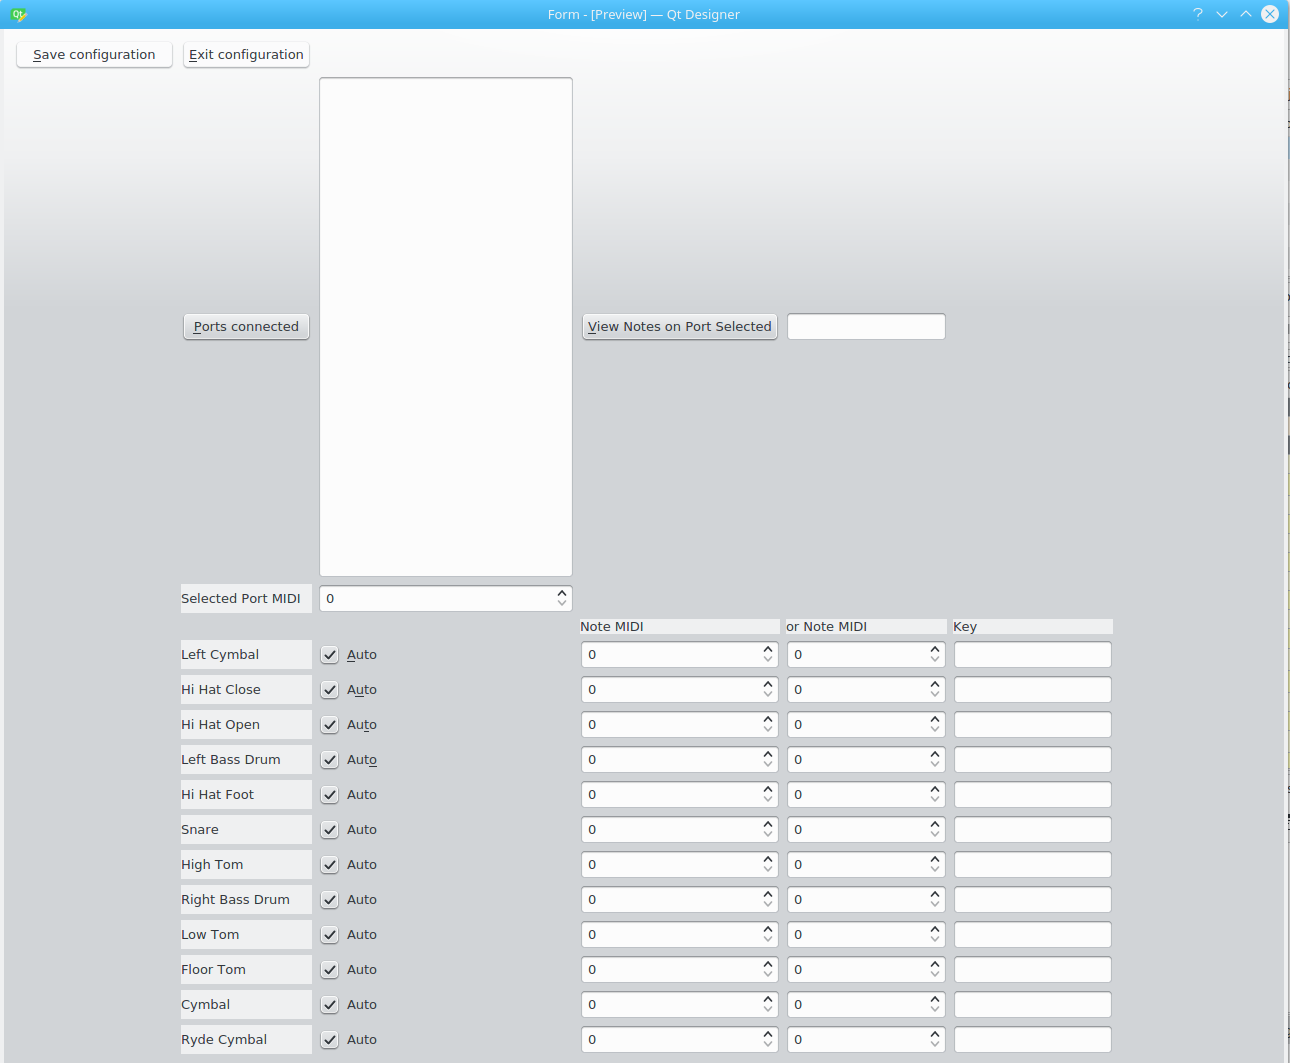
\includegraphics[scale=0.4]{Imagenes/WidgetConfigurarDrum.png}
% Ponemos Leyenda al gráfico
\caption{Widget Configurar Drum}
\label{Widget Configurar Drum}
\end{center}
\end{figure}


\subsection{MIDI} 
Antes de continuar se tiene que hacer una pequeña introducción a la comunicación MIDI enfocada a instrumentos-MIDI puros.

En la comunicación MIDI de un instrumento, hay mensajes diferenciados en 3 tipos:

\begin{itemize}
   \item Nota-on
   \item Variación de nota
   \item Nota-off
 \end{itemize}
 
y en cada mensaje hay la nota en sí, y su volumen.
 
Lo habitual es una Nota-on, y luego al cabo de X tiempo dependiendo del instrumento un Nota-off, dependiendo del instrumento se puede meter una o varias variaciónes de la nota antes de emitir el Nota-off.

Estos mensajes según el instrumento puede ser múltiples, ya que ese instrumento esta pensado para estar sonando varias notas al mismo tiempo, esto se suele determinar por el instrumento en sí  o por limitaciones del sintetizador MIDI que normalmente tienen un limite de notas al mismo tiempo.

En el proyecto por simplicidad y por como suele funcionar una batería, solo miraremos los mensajes tipo Nota-on.

Cada Intrumento-MIDI no emite sonidos, emite estos mensajes y es el sintetizador MIDI que teniendo sus bancos de sonidos configurados, puertos y notas es el encargado de reproducir los sonidos.

Pensar que este pyDTX, es la mezcla de un sintetizador enfocado a estos instrumentos-MIDI y a estos ficheros .dtx como partitura.

\subsection{Configuración MIDI en pyDTX}
Se tiene que exponer uno de los primeros problemas con el MIDI y su tratamiento.

Gracias a usar las librerías Qt, estas mismas librerías se encargan de que los eventos del teclado y ratón solo disparen los objetos gráficos visibles, pero si queremos implementar eventos MIDI, el programa tiene que saber que widget esta activo o solo implementar la escucha de los mensajes MIDI en parte de reproductor.

La manera que se ha resuelto es la siguiente, cada vez que estamos en un widget que tiene que escuchar los mensajes MIDI, se tiene una función que se llama al entrar en el widget (recordar que los widgets están creados todos al inicio para mejorar la fluidez del programa). En este widget de configuración de la batería-MIDI se ha resuelto esta problemática con un botón que es el que activa el escuchar los mensajes-MIDI y lo tenemos que desactivar siempre cuando volvemos al menú principal.


\subsection{Baterías-MIDI y Lanes}
Aunque lo mejor seria que el número de lanes visuales de los .dtx a tratar fueran los mismos que el número de Notas MIDI a configurar, ya que se podría hacer una relación uno a uno. Se tiene que tratar varios casos distintos bastantes comunes.

El número de lanes que se trata como lanes visuales son 12. Aunque visualmente solo tenemos 9 columnas visuales ya que hay lanes que comparten columna visual y los chips de estos lanes visualmente son de colores distintos para diferenciarlos.

La lista completa de los lanes visuales tratados es la siguiente:

\begin{itemize}
   \item 1A Left Cymbal
   \item 11 Hi Hat Close
   \item 18 Hi Hat Open
   \item 1C Left Bass Drum
   \item 1B Hi Hat Foot
   \item 12 Snare
   \item 14 High Tom
   \item 13 Right Bass Drum
   \item 15 Low Tom
   \item 17 Floor Tom
   \item 16 Cymbal
   \item 19 Ride Cymbal
 \end{itemize}

Conviene hacer un pequeño repaso de como se fue ampliando los 6 lanes visuales del inicio del formato .dtx hasta los 12 actuales (recordar que la maquina actual del gitadora solo tiene 7 pads y doble pedal).

Los primeros cambios ya fue separa el Hi-hat en posición abierto o cerrado, dependiendo del número de pads de la batería-MIDI y su capacidad, se necesitaría tocar de manera distinta o solo era una marca visual de que son notas distintas, como nunca se puede tocar el hi-hat al mismo tiempo en abierto y en cerrado se puso en la misma columna visual.


El siguiente cambio fue en los platillos, originalmente solo existía el lane 16 colocado a la derecha, se añadieron los lane 1A y 19 se definió el lane 1A como el platillo izquierdo y el 19 Como el platillo derecho.
Para no perder la compatibilidad con los .dtx anteriores a este cambio, se dejo el lane 16 a la derecha de todo. Aunque la maquina de Gitadora solo tiene 1 pad simple para el platillo izquierdo y otro pad simple para el platillo derecho. 

Si se reproduce un .dtx, anterior a este cambio se observaran el sonido de los platillos siempre a la derecha, pero el usuario no vera ninguna diferencia.

Como este lane no se ha desactivado, son los autores de los .dtx quienes tiene que escoger como usar este lane 16. 

Hay tres principales maneras de entender este lane antiguo en canciones más complicadas, la primera y mas sencilla es ignorarlo y emplear solamente los lanes de platillo izquierdo o derecho, la segunda opción es usar este lane antiguo como un tercer platillo adicional y la tercera opción es como este lane esta a la derecha junto al platillo derecho, emplearlo para tener dos notaciones en este lane de esta manera se puede simular y mostrar con una marca visual el tocar arriba del platillo o el tocar más al borde. 


En este proyecto por simplicidad se han juntado en la misma columna el lane 16 y 19, se marcan con notas de colores distintos pero no esta contemplado el caso de que haya al mismo tiempo dos notas simultaneas para estos dos lanes.

Cuando salio el gitadora se amplio la máquina árcade un doble pedal para ello se insertaron los Lane 1B y el 1C que serian los dos para el pie izquierdo, tanto para el hi-hat como para el doble bombo, como no es habitual tener una batería-MIDI con triple pedal y ya que lo más común es tocar canciones con doble bombo o usar el pie izquierdo para el Hi-hat, aunque a nivel visual comparten la misma posición y en el gitadora comparten color, se ha decidido igual que en el caso anterior hacer que las notas visualmente serán de colores distintos para las canciones donde si que hay tanto doble bombo como hi hat,y de esta manera saber visualmente que son notas distintas y si se tiene una batería-MIDI más cercana a una batería acústica con estas características poder tocar exactamente como en la batería acústica.
 
Ya que hay multitud de baterías-MIDI en el mercado se ha de tratar dos principales problemas:

Cuando hay menos pads que lanes o al revés y los dos casos tienen sus complicaciones, que ahora se expondrán.
 
\subsubsection{Pocos Pads para muchos lanes} 
El primer caso se solventa dejando que se pueda configurar una nota-MIDI en múltiples lanes, esto complica saber la sincronización de cuando se activa esta nota-MIDI con los lanes asociados.
Ya que esta configuración obliga a cuando se dispara la nota-MIDI comprobar en varios lanes si hay notas, para ello se tendrá que comprobar en todos los lanes asociados, y como suponemos la mejor sincronización posible solo se pondrá a hit el mejor tiempo de todos los lanes asociados, también hay que tener cuidado ya que hay canciones donde puede ser que se tengan que tocar estos dos lanes simultáneamente, y si hemos configurado estas dos lanes en la misma nota-MIDI serán dos hits.

\subsubsection{Muchos Pads para pocos lanes}

El otro caso es tener una batería-MIDI muy completa, y querer usarla para tocar los .dtx, si solo se puede configurar una nota-MIDI para cada lane, esto obliga al batería a tener que ser muy exacto ya que todos los pads con zonas múltiples, solamente se deberían tocar en una zona concreta, la solución más simple es dejar que en cada lane, se puedan configurar dos notas-MIDI al mismo tiempo.

\subsubsection{Casos especiales por respetar los dos al mismo tiempo}

Estos casos independientemente tienen su sentido pero el tener que respetar los dos al mismo se tiene una serie de ventajas y desventajas.

La desventaja clara es que nos complican el comprobar la sincronización entre tocar notas-MIDI y su relación con los chips de la partitura.

La ventaja de tener estas opciones además de las comentadas es que con el mismo programa no tendremos problemas a la hora de poner canciones del dtxmania original, dtxmaniaHD o del gitadora.

Ya que el principal inconveniente era el doble bombo, si se tiene una batería-MIDI con el doble bombo. 
Se puede configurar de la siguiente manera: el hihat y el bombo izquierdo se configuran en el pie izquierdo, pero además este pie izquierdo se puede poner también en el bombo derecho, con esto se ha conseguido que en la misma configuración poder llamar a canciones antiguas del dtxmania original, con doble bombo y se puede tocar con los dos pies, aunque no se respeta izquierda o derecha ya que esta asociado al mismo lane y debe ser el que toca saber que pie debería ser tocado. 

Con la misma configuración si la usamos para un dtx del dtxmaniaHD o del gitadora como estos ya diferencia pie izquierdo y derecho, la podemos usar y el pydtx indicara visualmente que pie se debería tocar, aunque con esta configuración en concreto se puede tocar el lane del bombo derecho correctamente o usar el pie izquierdo. Por lo que se observa que no hay manera de respetar todos los casos posibles y con una sola configuración obligar al mismo tiempo que la pulsaciones en los pads sean las que tendrían que ser en una batería acústica.

\section{Pantalla configuración pyDTX}
En este widget se dejara las opciones para que usuario configure los valores por defectos del pyDTX.

El usuario puede configurar el directorio donde se buscara el tema gráfico del pyDTX.

También se puede configurar el directorio inicial donde se buscaran los subdirectorios que interiormente tienen las canciones de dtx, detallar que por comodidad a la hora de navegar si queremos ir a un directorio superior de este directorio inicial se volvera a ir al menú principal.

Aunque se dejara cambiar la velocidad de sincronización antes de reproducir cualquier canción, se tiene una velocidad por defecto para ya tenerla configurada cada vez que se arranque el pyDTX.
Para tener claro que relación hay entre esta velocidad, que es el tiempo que tardara un chip en recorrer la pantalla desde el punto más alto a la parte inferior, y los tiempos de sincronización se pondrán unas indicaciones en pantalla para saber los margenes que se aplicaran para las posibles sincronizaciones Perfect, Great, Good y Poor.

Se creara la opción para seleccionar si para las animaciones de los chips gráficos durante la reproducción de la canción usaremos OpenGL, ya que esto es una asignatura pendiente en muchas plataformas arm y si obligamos a usar OpenGL, como se crean todas los widgets al inicio para mejorar los tiempos, el programa fallaría sin ni siquiera ver la pantalla de inicio (de todas maneras se puede cambiar el fichero de configuración ya que es un fichero de texto con extensión .ini)
 
\begin{figure}[H]
% Centramos la figura
\begin{center}
% Incluimos el gráfico y definimos el ancho y alto
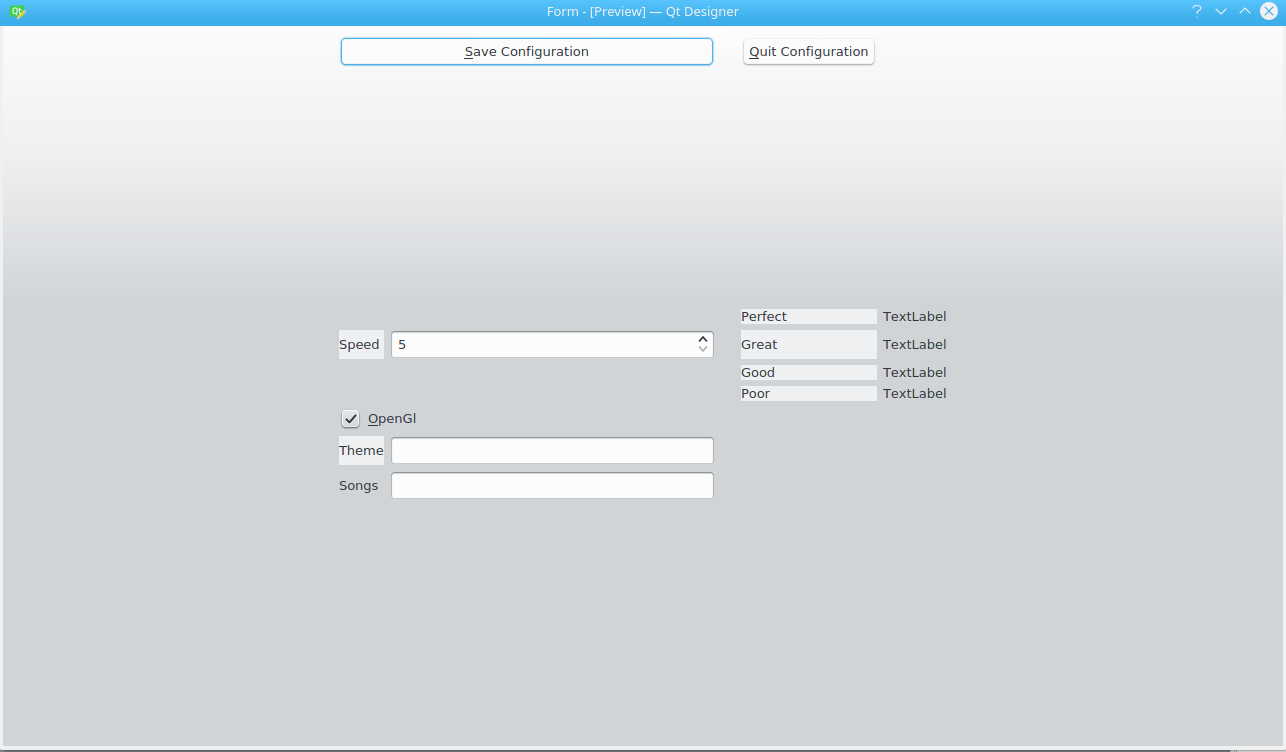
\includegraphics[scale=0.4]{Imagenes/WidgetConfigurarDTX.png}
% Ponemos Leyenda al gráfico
\caption{Widget Configurar DTX}
\label{Widget Configurar DTX}
\end{center}
\end{figure}
 
\section{Pantalla Navegación}
Se tiene que definir el  widget que el usuario empleara para seleccionar la canción a reproducir. Se copiara en medida de lo posible la navegación que se usaba en el dtxmania original, para ello este widget se dividirá en tres grandes partes, información de la canción actualmente seleccionada, una botonera para cambiar entre canciones o directorios, y una lista de los directorios y canciones del directorio seleccionado actualmente.

\begin{figure}[H]
% Centramos la figura
\begin{center}
% Incluimos el gráfico y definimos el ancho y alto
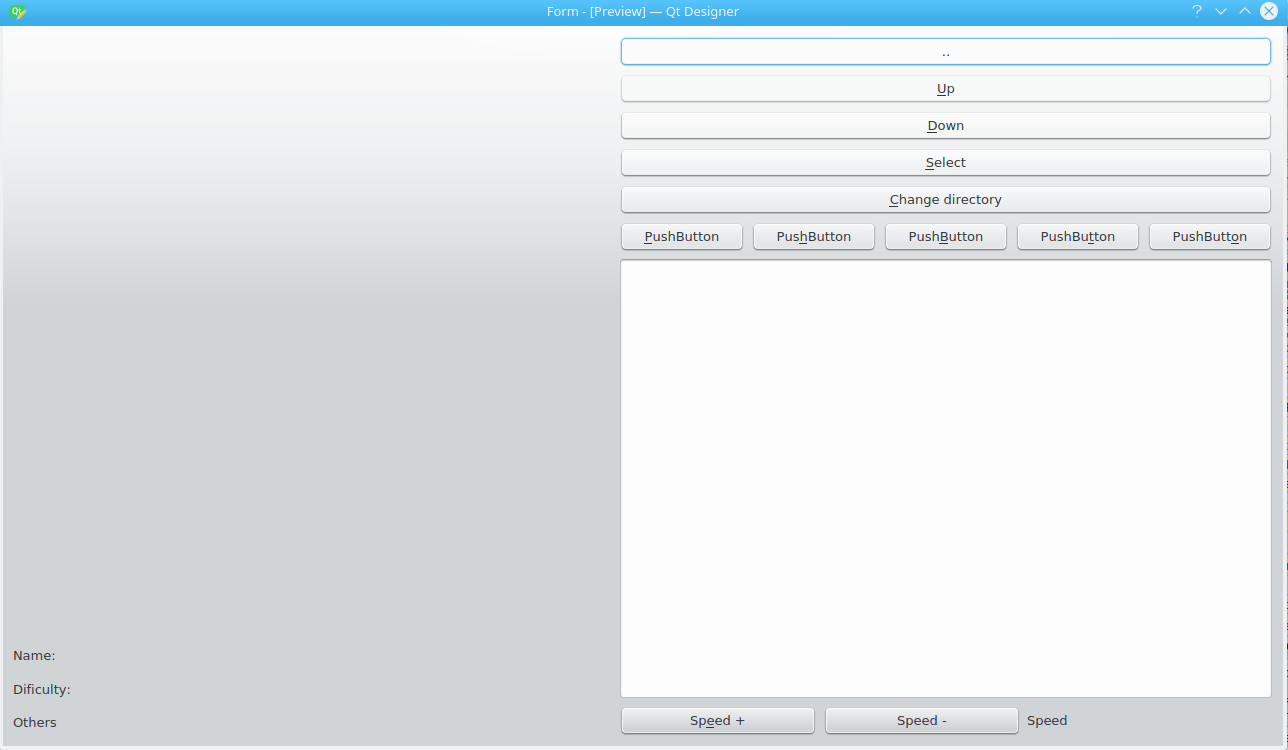
\includegraphics[scale=0.4]{Imagenes/WidgetNavegacion.png}
% Ponemos Leyenda al gráfico
\caption{Widget Navegacion}
\label{Widget Navegacion}
\end{center}
\end{figure}

Tenemos que definir más en detalles estas tres partes:

\subsubsection{Información de la canción}
Sera una columna a la izquierda donde se pondrá la información de la canción seleccionada, hay espacio para una imagen y varios textos (etiquetas gráficas en Qt5) para indicar autor de la canción, dificultad y uno de información extra.

Se tendrá en cuenta cada vez que se cambie el directorio o la canción seleccionada actualizar estos cuatro elementos gráficos.

\subsubsection{Lista de las canciones y directorios actuales}
A la derecha de la información gráfica y abajo de la botonera.

Se obtendrá la información de todos los subdirectorios que estén dentro del directorio actual de canciones, cuando se crea el widget sera del directorio indicado en la configuración.

Para una mayor comodidad en la navegación se entenderá que un directorio que tenga un set.def o un único .dtx contiene al menos una canción (esto se indica por el posible caso de varios .dtx pero ningún set.def).

Si solo hay un .dtx es tan sencillo como obtener la información del .dtx y ponerlo en la lista de selección, y si tiene un set.def obtener la información de los posibles cinco labels y de sus cinco posibles .dtx asociados.

Esta parte sera la encargada de tener una lista de los directorios actuales, cada ítem de esta lista sera uno de los siguientes casos:

\begin{itemize}
   \item Si dentro del directorio hay un set.def, se obtendrá una lista de 5 elementos, las 5 posibles etiquetas de estos elementos y la información de los .dtx asociados.
   \item Si no tiene un set.def se buscara un .dtx dentro del directorio y el primero que se encuentre se pondra la información de esta canción (la información para los 4 elementos gráficos).
   \item Si es un directorio sin set.def o .dtx, guardaremos su path.
 \end{itemize}
 
 
De esta manera tendremos una lista con toda la información del directorio actual ya guardada en memoria para no tener que estar pidiendo la información al sistema operativo, mientras que el usuario no se mueva de este directorio.

\subsubsection{Botonera para cambio de directorios o seleccionar canciones}
A lar derecha de la información gráfica y en la parte superior se colocaran los botones para poder navegar en la estructura de directorios.

En esta parte se colocaran los botones para realizar acciones sobre la canción seleccionada, velocidad de sincronización o sobre los directorios.

Comentar que no siempre veremos todos los botones ya que es más intuitivo si los botones que no tienen sentido, se esconden y solo se muestran los botones que si pueden realizar acciones sobre el directorio o canción seleccionada.

El primero y más sencillo es el botón de ir a un nivel de directorio superior, si lo usamos y ya se esta en el directorio configurado como directorio de las canciones volveremos al menú principal, si no subiremos un nivel el path de directorio y volveremos a crear toda la lista de directorios y canciones del directorio actual.

Se crearan dos botones para subir o bajar en la lista de directorios/canciones, ya que de esta manera se deja abierto la manera de seleccionar estos directorios, se dejara seleccionar vía ratón pero también se puede seleccionar vía teclado, mediante la tabulación entre botones, recordar que de esta manera sera sencillo hacer que una batería-MIDI simule estas ordenes si solo dejáramos la vía del ratón, se debería cambiar mucho código para que funcionara mediante la batería-MIDI.

Abajo se crearan dos botones para variar la velocidad de sincronización actual y un elemento gráfico para ver la sincronización actual. De esta manera el usuario no tiene que ir hasta al menú de configuración para cambiar el valor de la sincronización.

Se creara un botón para reproducir la canción actual, este botón solo se mostrara en el caso de que estemos seleccionando un directorio que no tiene un set.def y al menos tiene un .dtx, cuando se pulsa empezaremos a reproducir la canción con la velocidad de sincronización actual.

Se creara un botón para cambio de directorio, solo se mostrara si estamos seleccionado un directorio sin set.def o .dtx, si se pulsa cambiaremos de directorio y se tendrá que rehacer toda la lista de posibles directorios/canciones

También se tiene cinco posibles botones para los directorios que tienen un set.def, como el programa original no indicaba nada en las canciones que hay por internet estos cinco posibles .dtx no tienen un orden ya que dependía del creador de los .dtx y del set.def cuantos y como se empleaban estas cinco posibilidades (hay canciones en internet que solo definen el segundo label y el tercero por ejemplo), en cada una de estas posibilidades se puede apuntar a un .dtx y poner un texto para información, además de la información que tiene el .dtx.
Para ello cuando se crea la información de un directorio con un set.def se obtendrá toda la información disponible y también indicar donde no se ha  podido obtener, para mostrar solamente los botones que tienen asociada información.

Se actualizara la información mostrada de la canción con el primer botón que tiene asociada información.
 
Se ha tenido que usar una opción del Qt5 para cuando hay focus en uno de estos botones ya que se tiene que actualizar toda la información mostrada de la canción seleccionada.

Esto se ha realizado de esta manera para integrar el uso del ratón y del teclado o posible batería-MIDI ya que si solo se tiene en cuenta el ratón siempre se pulsaba directamente los botones y no se podía ver la información de los .dtx, o se tendría que haber puesto dos botones más para poder navegar entre los posibles .dtx de un set.def, se ha preferido para simplificar el menú mediante esta reprogramación de los eventos si hay focus en uno de estos botones, poner la información del .dtx relacionado.

\section{Reproducción de la canción}

\subsection{Inicialización básica y detalles de Qt5}
El widget donde se reproducirá la canción seleccionada, sera un widget gráfico ya que sera el encargado de tener los lanes visuales y dentro de ellos los chips visuales, además del widget de puntuación.

Este widget gráfico ya estará creado, y según la configuración se usara OpenGl o no, se tiene que desactivar las opciones del qt5 de las barras de scroll del QgraphicsView, ya que por defecto si se añaden elementos gráficos en los limites de la visión, aparecerían barras de scroll para poder ver todo.

Otra cosa a evitar es el evento resiseEvent, ya que si se redimensiona la pantalla, se ha pensado que siempre estaremos usando la misma resolución interna, de esta manera sera el Qt5 el encargado de mantener la relación de aspecto.

No se puede inicializar nada más ya que se depende de la canción seleccionada y del tiempo de sincronización.

\subsection{Inicialización con una canción}
Cuando se llama a este widget con un .dtx concreto y una velocidad de sincronización. Es cuando se tiene que reproducir el dtx, para ello se tiene que hacer varias tareas que paso a describir.

Se tiene que leer los ficheros de configuración, para tenerlos en memoria.

Como toda la parte gŕafica sera mediante Qt5, se crea una scene y se ira añadiendo los elementos gráficos a esta scene para que Qt5 sea quien los pinte.

Se tiene que configurar el teclado y el instrumento MIDI.

\subsection{Teclado}
\subsubsection{Configurar teclado}
Se crea un diccionario donde se guardara la relación de teclas con su lane correspondiente.

Recorriendo todas las lanes visuales, se comprueba si la lane esta configurada sin automático, si fuera de esta manera se inserta su tecla asociada a su lane en este diccionario de teclas. 

\subsubsection{Evento de teclado}
Se configura el evento keyPressEvent de Qt5, para que cuando se pulse una tecla lancé este evento.

Se comprueba si es la tecla especial Escape, si fuera esta se tiene que parar la reproducción actual y volver a el menú de selección de canciones.

Si no fuera así, se comprueba que tecla se ha pulsado y si esta en el diccionario de teclas que se ha configurado, se tiene que comprobar el tiempo actual y comprobar la puntuación en el lane asociado, esto se explicara más concretamente cuando definamos los lanes visuales y que funciones tienen.

\subsection{MIDI}
\subsubsection{Configurar MIDI}
Se crea un diccionario donde se guarda las notas midis y la lista de sus lanes correspondientes.

Recorriendo todas las lanes visuales, si la lane esta configurada sin automático, se comprueba su dos posibles MIDI y entonces se añaden a este diccionario de MIDI, con cuidado ya que una nota MIDI puede activar múltiples lanes, por eso en este caso son listas dentro de un diccionario y no un diccionario simple.

\subsubsection{Evento MIDI}
Mediante rtmidi2 se define una función que se dispara cada vez que vea un evento MIDI, del instrumento MIDI que esta en la configuración.

Cuando se dispara este función es comprobar el tipo de mensaje MIDI que tiene, los eventos tipo '153' Note-On serán los que se traten.

Si fuera de esta manera, se comprueba si la nota de este evento esta definida dentro de nuestro diccionario.

Aquí hay que tener mucho más cuidado que con el teclado ya que hay dos posibles casos:
Que haya solamente un lane asociado a esta nota-midi por lo que es lo mismo que el caso con el teclado o, puede ser que haya varios lanes asociados a esta nota-midi por lo que se tendrá que hacer una doble pasada sobre los lanes asociados: una primera para obtener el tiempo menor comparando con el tiempo actual, para saber a que lanes iría esta nota, y luego ya ir a los lanes y marcarlos como hit, recordar que pueden existir notas en varios lanes en el mismo tiempo. 

\subsection{Lanes}
 Una vez configurados los métodos de entrada teclado y midi. Se tiene que crear los lanes tanto automáticos como visuales.

\subsection{Ideas básicas de los lanes}
Se entiende un lane como una lista de chips, los lanes se separan en dos grandes grupos lanes automáticos y lanes visuales, los cuales tendrán a su vez asociados chips auto y chips visuales, pasamos a describir los chips ya que son más sencillos y luego se describirán con más exactitud los lanes.

\subsubsection{Chips Auto}
Se tiene que crear una clase Chip Auto.

Los chips auto son los chips que tendrán los lanes automáticos puros, que son los que se emplean para o poner la música de fondo o para ir añadiendo sonidos simples en la canción, ejemplo clásico metrónomo para canciones de practica.

Un chip auto es una nota (un sonido que estará en un banco de sonidos definido en el dtx) y un tiempo donde debería ser tocada.

Se crearan dos funciones en esta clase para leer el tiempo y su nota en sí.

\subsubsection{Chips Visuales}
Se crea una clase que se extiende de QGrapchicsWidget, para que Qt5 pueda manejar toda la parte gráfica y se pondrán los mismos datos y funciones que la clase Chip Auto.

Esta clase es un tipo de Chip pero visual, donde además de la información anterior si tiene que tener la información de si el chip ya ha sido pulsado, una animación, un color de chip y una posición horizontal en pantalla.

Los datos de color y posición son dependientes del lane donde estará este chip.

Las funciones que se definen además de las de un chip auto son:


paint: función que usara Qt5 para pintar este chip en concreto donde se indica que pinta un rectangulo, con un color.

animar: función donde se tienen que crear una propiedades de animación para que qt5 lo trate, básicamente es poner un chip, arriba de la pantalla con su posición horizontal de la lane donde está e indicar que tiene que acabar esta animación en la misma posición horizontal pero al final de la pantalla, indicando que tiene que tardar el tiempo de sincronización.

Esta función tiene que devolver la animación en sí, ya que sera la scene de Qt5 donde se tiene que tratar.

\subsubsection{Lanes Auto}
Se creara una clase lane Auto donde se tendrán dos datos una lista de chips, y un banco de sonidos.

Las funciones asociadas a esta clase son las siguientes:

insertar\_chip: Para poder insertar chips en la lista de chips.

insertar\_sonidos: Para poder insertar el banco de sonidos en la lane auto.

reproducir: Donde se buscara el primer chip de la lista y si su tiempo es igual o menor al tiempo actual, se tendrá que reproducir su nota asociada y eliminar este chip.

\subsubsection{Lanes visuales}
Extendiendo la clase de Lane Auto se definirá la clase Lane visual estos lanes, tendrán una lista de chips y una función para reproducir los sonidos por si estuvieran configurados como automático, se tendrá que añadir toda la información gráfica y funciones para comprobar la puntuación obtenida según el sincronismo.

Los datos de un lane visual son los de un lane automático y además color, posición horizontal y el tiempo de sincronización, de este último se calcula el tiempo máximo a mantener una nota en memoria, ya que una nota que ya ha pasado su tiempo donde tendría que haber sido tocada y el margen de puntuación en ``poor'', esa nota es un  ``miss'' y se puede borrar de memoria.


Además de funciones para leer datos del estilo leer\_color y leer\_pos.

Hay tres funciones adicionales para estos lanes visuales:

comprobar\_y\_poner\_hit:

Función para buscar la nota más cercana al tiempo actual, y ponerla a hit, se devolverá la diferencia del tiempo actual al tiempo de la nota, para poder puntuar.

comprobar\_tiempo:

Función que se usara para cuando una nota-midi esta en varios lanes visuales, se comprueba en la lista la nota más cercana al tiempo actual y se devolverá el tiempo de diferencia; de esta manera se podra saber el lane donde esta la nota más cercana.


eliminar\_nota\_antigua:

Con el tiempo actual se comprueba si la primera de la lista ya ha superado su tiempo y el tiempo de margen de hasta una nota en calificación ``poor'', se borra esta nota de las lista de notas si ha superado este tiempo. Y se devuelve true si se ha eliminado una nota que no haya sido pulsada, esto es para poder indicar a la puntuación que hay una nota más en miss.

\subsubsection{Reproducir una canción}
Ahora que se han definido tanto los chips como los lanes, se puede indicar tranquilamente que se tienen que crear los lanes automáticos, 01, 61 y 62, que son los lanes automáticos más comunes en los .dtx. y los se ponen en un diccionario de lanes automáticos.

Se crean los lanes visuales 11, 12 , 13, 14, 15,16,17,18,19 ,1A, 1B y 1C con sus colores y posiciones, siempre mirando si en la configuración esta puesto como lane automático, si fuera de esta manera además de en el diccionario de lanes visuales, se tendría que añadir también al diccionario de lanes automáticos.


Se pone el número de compases a cero, y se tiene que obtener la información básica del .dtx, para ello se tendrá que hacer varias pasos.


En el primer paso se obtendrán los siguientes datos:

Todos los bancos de sonidos que están definidos como ordenes WAVxx, si el sonido es un .ogg o un .wav se creara un banco de sonido con un reproductor asociado al tipo del sonido; de esta manera cuando se tenga que reproducir el sonido ya estará cargado en memoria y preparado.

Toda la información de los posibles cambios de BPM en la canción y de los BPM por defecto.

Se obtendrá la información del nombre de la canción para ponerlo en el widget de la puntuación.

Se ira tratando la información de los compases poco a poco para ello, primero obtendremos sus notaciones, en que lane son estas notas y en que compás.

Como todas las notaciones deberían estar colocadas por compás y no hace falta que estén ordenadas por lane, lo que se hará mientras se recorren todas las notaciones en el archivo .dtx es lo siguiente, si es un compás mayor que el actual se pondrá en esta lista de compases en el sitio del compás un diccionario con la key 'lanes' vacía, y luego se insertara los datos en el compás, y en este diccionario ya se pone usando la lane como key, las notaciones u ordenes sin tratar todavía(tal y como están en el archivo .dtx), también recordar que en los ficheros .dtx se pueden saltar compases si no hay ninguna nota en esos compases, pero para el proyecto ya se crea en esta lista de compases, compases que internamente tendrá una key 'lanes' pero no llegaran a tener notaciones internas.

Ahora ya se tiene una lista de compases y en cada compás un diccionario con una key 'lanes', y con las notaciones separadas por lanes.


Ahora creamos la puntuación.
\subsubsection{Puntuación}
Usamos un widget por comodidad, donde tendremos los siguientes datos:

Datos visuales:
Titulo de la canción
Número de notas en perfect
Número de notas en great
Número de notas en good
Número de notas en poor
Número de notas en miss
Número de notas en combo
Número de notas máximas en combo

Datos a guardar en este widget:
Los tiempos de margenes calculados a partir del tiempo de sincronización.

\begin{figure}[H]
% Centramos la figura
\begin{center}
% Incluimos el gráfico y definimos el ancho y alto
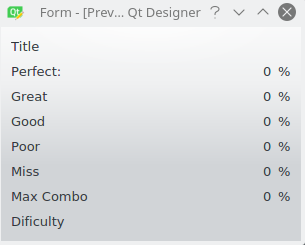
\includegraphics[scale=0.8]{Imagenes/WidgetPuntuacion.png}
% Ponemos Leyenda al gráfico
\caption{Widget Puntuación}
\label{Widget Puntuación}
\end{center}
\end{figure}


Con las siguientes funciones:

comprobar\_puntuacion:
Con el tiempo de margen que nos pasan, se miran los tiempos de sincronización y se actualizan los datos en consecuencia.

actualizar\_puntuacion:

Función para actualizar los elementos gráficos de la puntuación.

aumentar\_miss: 
Función que se empleara cuando hay una nota que se tiene que eliminar por tiempo, ya directamente se sabe que es un miss.


\subsubsection{Continuamos actualizando los compases}

Insertamos los bancos de sonidos en todos los lanes.

Ahora se tiene que poner en todos los compases los tiempos, para ello se ira recorriendo la lista de compases y si hay una nota en los lanes 03 o 08 ya que estos modifican los BPM de la canción; lo más habitual es que se cambie al inicio del compás o justo en la última nota del compás para el compás siguiente, se ha implementado tanto el lane 03 como el 08, ya que aunque parece que se quiere dirigir el formato hacia cambios absolutos, para tener retrocompatibilidad se ha implementado los cambios de BPM con sumas o restas al BPM actual, para ello en el diccionario que es el compás actual ahora añadimos dos keys, que son la key 'bpm' asociada al bpm del compás actual y la key 'tiempo' que es el tiempo donde se debería iniciar el compás según el .dtx.

Ahora se tiene que recorrer otra vez la lista de compases y ahora se puede coger todas las notaciones de los lanes y compases, y separarlos en notas con un tiempo, quitando las notas 00 que son silencios en los .dtx.

Se crea un evento para salir del reproductor cuando se acabe el tiempo de la canción más el doble tiempo de sincronización, para tener un margen extra.

Se inicia el control del tiempo, ya que se tiene todos los datos ya tratados para comenzar la reproducción del .dtx.

Se anima el primer compás, ahora se explicara que se considera animar un compás, se quita de la lista de compases pasándolo a ser el compas que se esta comprobando actualmente, y se pasa al bucle principal de la reproducción, usando un timer de Qt5 para cada milisegundo volver al bucle principal.


\subsubsection{Animar un compás}
Para animar un compás en la reproducción de un .dtx, se necesita un compás, y el tiempo actual.

Para animar el compás actual lo que se tiene que hacer es repasar todos sus lanes, mirar la primera nota de cada uno de esos lanes y si su tiempo es menor que el tiempo actual, quitarla del compás a animar y pasar esta nota a su lane correspondiente modificando el tiempo de esta nota (sumando el tiempo de sincronización), pensar que se estará animando este compás mientras no se llege al tiempo del siguiente compás.

Hay que separar las notas en dos grandes grupos:

Las que están en lanes puros automáticos (01,61 y 62).

Y las notas para los lanes visuales, en este caso se tendrá que crear una nota visual con sus propiedades gráficas dependiendo del lane y añadirla a la scene asociada al Qt5.

Si fuera una nota no asociada a ningún lane implementado se pondrá esta información en el terminal.

\subsubsection{Bucle principal de la reproducción}
En el bucle principal de la reproducción se tiene que hacer varias cosas:

Coger el tiempo actual, continuar animando el compás actual, ya que puede tener todavía notas a animar.

Comprobar que no se esta en el tiempo del siguiente compás. Si fuera de esta manera se actualiza el compás actual y se quita de la lista de compases.

Se da la orden de reproducción en todos los lanes auto, tanto los puramente auto como los configurados por el usuario.

Se comprueba que no se tiene que eliminar ninguna nota por tiempo, en los lanes visuales.

Y se vuelve a usar un timer de Qt5 para hacer una parada en la CPU y que Qt5 pueda actualizar todos los elementos gráficos y después se volverá a llamar a este bucle principal.

\chapter{Detalles de la implementación}
\section{Transformar .dtx a .dtx libre}

La idea es bajarse canciones de internet y ejecutando alguno de los dos scripts de transformar a .dtx libre estos se encargaran de varias tareas:

\begin{itemize}
   \item Codificar los .dtx en utf-8
   \item Transformar los .xa a wav
   \item Transformar los .mp3 a .ogg
   \item Cambiar internamente los .dtx apuntando a estos archivos en formatos libres
 \end{itemize}

Se dan dos posibles scripts ya que hay .dtx que tienen los sonidos .xa o .wav dentro de una subcarpeta para mejorar la estructura de ficheros.

Las canciones tendrían que estar dentro de la carpeta que contiene estos scripts ya que el wine necesita tener los path relativos para encontrar tanto los ficheros a transformar como el xa.exe para poder transformar de .xa a .wav.

\section{DRUM-HAT MIDI}

Se ha conseguido un código independiente que si esta en cpu al mismo tiempo, que el pyDTX, el Drum-HAT emite señales MIDI que se pueden tratar en este o otros programas que reciban información MIDI.

\section{pyDTX}

Se ha configurado un script de python con la opción de optimización, para que se mejore en lo posible la ejecución, viendo las ideas generales, el mayor problema de este proyecto es el buen uso de los timers y de la capacidad de la cpu para reproducir simultáneamente todos sonidos en los lanes, de esto se encargara las librerías Qt5, en segundo plano queda el tema gráfico que también se encarga el Qt5.

Son las librerías Qt5 que según su código y sistema operativo donde se esta ejecutando, según los recursos disponibles obtendrán acceso a la pantalla y al sonido. 

Se ha implementado el control MIDI vía Cython por lo que esta bastante optimizado.

La programación se ha realizado de tal manera que siempre el sonido tiene prioridad, sobre los gráficos.

Debido al poco uso de dobles lineas en un .dtx para un mismo compás y lane en concreto, no se ha implementado, aunque este descrito en el formato, la descripción no indica que hacer si por error se crean dos notas al mismo tiempo en el mismo lane.

\section{Instalación}

\subsection{Fedora 25 - x86 64bits}
En una distribución fedora 25, las librerías necesarias y sus instrucciones para instalarlas son las siguientes:

\begin{Verbatim}[frame=single]
    sudo dnf install alsa-lib-devel  
    sudo dnf install python3-Cython 
    sudo dnf install rtmidi-2*
    sudo dnf install rtmidi-devel-
    sudo dnf install redhat-rpm-config  
    sudo dnf install gcc-c++
    sudo pip3 install rtmidi2
\end{Verbatim}

En un linux mint se tuvo que añadir las siguientes librerías para poder compilar el Cython:

\begin{Verbatim}[frame=single]
sudo apt-get install python3-setuptools
sudo apt-get install g++
sudo apt-get install python3-dev
\end{Verbatim}


\subsection{Raspberry3 - armv7}

En la raspberry3 en la distribución Raspbian y ubuntu, están son las librerías a instalar para este proyecto:

\begin{Verbatim}[frame=single]
  sudo apt-get install librtaudio-dev
  sudo apt-get install librtmidi-dev
  sudo apt-get install librtmidi2   
  sudo pip3 install Cython 
  sudo pip3 install rtmidi2
  sudo apt-get install libqt5multimedia5
  sudo apt-get install libqt5multimedia5-plugins
  sudo apt-get install python3-pyqt5
  sudo apt-get install python3-pyqt5.qtmultimedia
  sudo apt-get install python3-pyqt5.qtopengl  
\end{Verbatim}

Indicar que la instalación de las librerias Cython dura unos 20 minutos.

En la distribución Raspbian la instrucción:
\begin{Verbatim}[frame=single]
  sudo apt-get install librtmidi2   
\end{Verbatim}

No es necesaria ya que en la instrucción anterior por dependencias ya se la instala pero se ha dejado para tener las instrucciones tanto en raspbian como en ubuntu en el mismo lugar.

\subsection{Conseguir el código fuente}

Para conseguir el código fuente del proyecto se puede usar las siguientes ordenes
\begin{Verbatim}[frame=single]
    git clone https://github.com/kapoira/pyDTX.git
\end{Verbatim}


Para conseguir el código fuente del script para transformar los .dtx de internet se puede usar la siguiente orden:

\begin{Verbatim}[frame=single]
  git clone https://github.com/kapoira/Transformar-DTX-libre.git
\end{Verbatim}

Si se quiere conseguir la utilidad para que el DrumHat genere señales MIDI, se puede obtener con la siguiente orden:

\begin{Verbatim}[frame=single]
    git clone https://github.com/kapoira/MIDI-out-DrumHat.git
\end{Verbatim}

\subsection{Problemas encontrados con .dtx de internet}
Se ha de comentar que además de no tener toda la documentación en ingles, ya que el autor ha ido ampliando el formato según quería adaptarlo a las nuevas versiones del dtxmania hd o del gitadora, el autor también ha ido añadiendo posibles comandos de los que no hay ninguna documentación.

Un claro ejemplo es el comando:

\begin{Verbatim}[frame=single]
#DTXC_CHIPPALETTE: 
\end{Verbatim}


Hay .dtx en internet donde no se cumple la documentación de los .dtx con errores del estilo:

No poner el caracter ``:'' cuando esta definido en la documentación ejemplo : \#L1LABEL en vez de \#L1LABEL:

Apuntar a canales de sonido no definidos en el mismo .dtx.

Todos estos errores no son tratados por el script que pasa de .dtx a .dtx libres, por lo que según que errores pueden hacer que este reproductor tenga fallos, se ha dejado la salida del terminal activa para poder tener controlados estos fallos y modificar el .dtx en consecuencia.

\subsection{Comentarios finales en la Raspberry}

Para que funcione en raspbian se tiene que llamar al demonio pulseaudio, y si además se quiere usar el drumHat al mismo tiempo, también se tendrá que llamar al programa MIDI-out-DrumHat.

En la raspberry3 este proyecto funciona pero el sonido se entrecorta, se puede usar como lector de partituras pero no se aconseja estar pendiente del sonido que saca la rapsberry.

Como se puede observar el código esta funcionando por lo que solo es cuestión de tiempo o de alguna de las siguientes opciones:
\begin{itemize}
  \item El interprete de python pypy3 tenga soporte para las librerias qt5.
  \item Raspbian tenga un kernel en arm64 (La raspberry3 tiene una cpu capaz pero por no tener que mantener doble código por ahora la comunidad oficial solo dan la opción de armv7).
  \item Se obtenga la aceleración OpenGL completa, de esta manera se liberara la cpu y se podrá mejorar los tiempos de latencia que afectan al sonido.
  \item Se mejore el pulseaudio en la distribución Raspbian (Raspbian por ahora soporta ALSA de base ya que consume menos recursos).
  \item Si sale una raspberry más potente.
\end{itemize}

También se podría probar en otros microordenadores como los ODROID, ya que estos tienen una cpu más potente que la Raspberry, aunque también se tendría que mirar su compatibilidad con OpenGL y las librerías Qt5.

\subsection{Comentarios finales al proyecto}
Ahora que se ha tenido que implementar un reproductor de .dtx en entornos libres, se han observado carencias en el formato o puntos flojos ya que se han ido añadiendo comandos a medida que pasaba el tiempo que no estaban pensados en un origen.

Aquí se expone una lista de posibles mejoras para un futuro formato.

\begin{itemize}
  \item Un detalle que poco a poco se han dado cuenta es evitar los formatos con DRM, aunque eso muchas canciones continúan usando los .xa o .mp3. 
  \item Referente a esto en los lanes visuales se suele usar sonidos del estilo rápido ya que es donde se colocan los sonidos de la batería, pero estaría bien tener un lane o varios que fueran específicamente para la música de fondo, de esta manera se simplificaría la parte de control de sonidos por si son .wav o .ogg.
  \item Simplificar el cambio de tempo dejando solo cambiar con valores absolutos, ya que es mucho más simple para el ordenador de programar.
  \item Se podría mejorar el tratamiento de los .dtx generando un fichero intermedio, ya que cada vez que queremos reproducir un .dtx, tenemos que repasar todo el .dtx para generar todos los compases, todas sus notas y asignar tiempos a estas notas, como todo esto no depende del tiempo de sincronización se podría crear un fichero que mientras no se modifique el .dtx asociado, y quitarnos tiempo de computación.
  \item Definir bien los lanes asociados a los platillos izquierdo y derecho, como ya se hizo con los pies, el problema de esto es que hay que rehacer canciones para tenerlas en el formato correcto.
\end{itemize}

\chapter{Posibles mejoras en el futuro}

Cuando se actualice la versión de python en las distribuciones de la raspberry, se podría actualizar la manera de revisar los ficheros existentes en los directorios de las canciones, fue un gran cambio en el paso a pyhton 3.5 pero no se ha usado en este proyecto para no dejar a las grandes distribuciones de raspberry colgadas.

El siguiente gran cambio en python 3.6 seria actualizar la manera de ver las notas ya que se actualizo la manera de entender los números ya que se contempla a partir de esa versión poner el carácter guión bajo para una mejor lectura de los números: 1\_000\_000 ahora se acepta como número y esta característica se podría emplear para limpiar la parte de coger objetos y notas de un .dtx.

Ampliar las ordenes del .dtx y los lanes implementados para tener un mayor porcentaje de compatibilidad con los .dtx que hay en internet.

Una opción que seria muy interesante y no esta implementada es conseguir que también en el menú de navegación de las canciones poder usar el instrumento-MIDI configurado como entrada para de esta manera poder arrancar el pyDTX y si esta la batería-MIDI bien configurada, poder usar todo el pyDTX sin dejar las baquetas.

Aunque se muestra la puntuación no se guarda en ningún sitio ni hay una pantalla de final canción para comprobar tranquilamente lo bien o mal, que se ha tocado una canción, aquí según como se quiera entender el aprendizaje de la batería se debería implementar de distintas maneras ya que la básica de solo guardar la puntuación máxima, y no poder ver que parte de la canción ha sido donde se ha fallado no es del todo correcta.

Actualmente no hay ninguna animación para cuando se toca un Pad, esto es bueno en el aspecto que minimiza todo el uso de cpu para carga gráfica pero estaría bien tener una animación para cada lane para poder comprobar que nivel de sincronización tenemos en cada nota, ya que en las notas dobles es difícil saber que nota es la que no se ha tocado bien.

No se analizan los box.def que pueden existir en las carpetas superiores de las canciones para tener o una imagen (de todo el álbum) o más información que solo el nombre de la carpeta.

Para dejar todo más elegante estaría bien poner también unos fondos de pantalla en las pantallas de configuraciones, dependientes del tema.

Un detalle para los baterías seria indicar al reproductor, que haga marcas visuales de en que compás esta la canción y marcar visualmente el inicio de cada compás.

Seria interesante implementar este proyecto usando QtQuick2 ya que Qt5 se esta enfocando en su lenguaje QML, más que en los widgets, de esta manera logran todavía más una mayor independencia del sistema operativo y en teoría una mejor optimización de los recursos empleados.

\appendix


\chapter{Código fuente}
\section{Transformar .dtx a .dtx libre}

\lstinputlisting[language=bash]{../Transformar-DTX-a-DTX-libre/Transformar-dtx-a-dtxlibre.sh}

\section{DRUMHAT en instrumento midi}

\lstinputlisting[language=Python]{../MIDI-out-DrumHat/MIDI-out-DrumHat.py}
\section{pyDTX}

No se indica el código fuente generado desde los .ui

\subsection{ChipAuto.py}

\lstinputlisting[language=Python]{../src/pyDTX/ChipAuto.py }

\subsection{Chip.py}

\lstinputlisting[language=Python]{../src/pyDTX/Chip.py }

\subsection{LaneAuto.py}

\lstinputlisting[language=Python]{../src/pyDTX/LaneAuto.py }

\subsection{LaneVisual.py}

\lstinputlisting[language=Python]{../src/pyDTX/LaneVisual.py }

\subsection{main.py}

\lstinputlisting[language=Python]{../src/pyDTX/main.py }

\subsection{UtilidadesDTX.py}

\lstinputlisting[language=Python]{../src/pyDTX/UtilidadesDTX.py }

\subsection{MyMainWindowQt5.py}

\lstinputlisting[language=Python]{../src/pyDTX/MyMainWindowQt5.py }

\subsection{MyWidgetConfigurarDrum.py}

\lstinputlisting[language=Python]{../src/pyDTX/MyWidgetConfigurarDrum.py }

\subsection{MyWidgetConfigurarDTX.py}

\lstinputlisting[language=Python]{../src/pyDTX/MyWidgetConfigurarDTX.py }

\subsection{MyWidgetNavegacion.py}

\lstinputlisting[language=Python]{../src/pyDTX/MyWidgetNavegacion.py }

\subsection{MyWidgetPuntuacion.py}

\lstinputlisting[language=Python]{../src/pyDTX/MyWidgetPuntuacion.py }

\subsection{ReproductorDTX.py}

\lstinputlisting[language=Python]{../src/pyDTX/ReproductorDTX.py }


\chapter{Guía de estilo python}
Aquí esta la guía de estilo que se utilizara durante el proyecto para escribir código, ya que de esta manera tanto la lectura, como el mantenimiento del código sera mucho más sencillo.
Uno de los grandes problemas de python es que no se esta obligado a seguir un estilo de programación, a la hora de escribir código se puede generar verdaderos desastres y si encima se junta que se puede crear variables en tiempo de ejecución y en mitad del código, mejor no pensar en las barbaridades con las que uno se puede encontrar.

Para ello se va a exponer las normas que se usaran para generar código python.

Una de las ideas es que el código se suele leer mucho más de lo que se escribe. Las guías de estilo que proporciona este documento están dirigidas a mejorar la legibilidad del código y hacerlo consistente a lo largo del amplio espectro del código python. Como dice el Zen de python, ``La legibilidad cuenta''.
Una guía de estilo nos ayuda a lograr consistencia. Ser consistente con esta guía de estilo es importante.
La consistencia dentro de un proyecto es aún más importante. La consistencia dentro de un módulo o función es la más importante.

Dos buenas razones para romper una regla en particular son:

\begin{enumerate}
\item Que al aplicar la regla el código se haga menos legible, incluso para alguien que esté acostumbrado a leer código que sigue las normas.
\item Para ser consistente con código relacionado que también la rompe (quizás por razones históricas) -- aunque esto también es una oportunidad de arreglar el desaguisado de otra persona (al más puro estilo XP).
\end{enumerate}

\section{Formateo del código}
\subsection{Indentación}
Usa 4 espacios por cada nivel de indentación

\subsection{Tamaño máximo de línea}
Limita todas las líneas a un máximo de 79 caracteres.

\subsection{Líneas en blanco}
Separa las funciones no anidadas y las definiciones de clases con dos líneas en blanco.

Las definiciones de métodos dentro de una misma clase se separan con una línea en blanco.

Se pueden usar líneas en blanco extra (de forma reservada) para separar grupos de funciones relacionadas. Las líneas en blanco se pueden omitir entre un grupo de funciones con una sola línea (por ejemplo, con un conjunto de funciones sin implementación).

Usa líneas en blanco en las funciones, de forma limitada, para indicar secciones lógicas.

\subsection{Codificación de caracteres}

Usaremos UTF-8

\subsection{Imports}
\begin{itemize}
\item Normalmente los imports deberían colocarse en distintas líneas, por ejemplo:
Sí:
\begin{lstlisting}
    import os
    import sys
\end{lstlisting}
No:
\begin{lstlisting}
    import sys, os2
\end{lstlisting}
aunque también es correcto hacer esto:
\begin{lstlisting}
    from subprocess import Popen, PIPE
\end{lstlisting}
\item Los imports se colocan siempre en la parte superior del archivo, justo después de cualquier comentario o cadena de documentación del módulo, y antes de las variables globales y las constantes del módulo.

Los imports deberían agruparse siguiendo el siguiente orden:
\begin{itemize}
\item   1. imports de la librería estándar
\item   2. imports de proyectos de terceras partes relacionados
\item   3. imports de aplicaciones locales/imports específicos de la librería
\end{itemize}
Deberías añadir una línea en blanco después de cada grupo de imports.

Si es necesario especificar los nombres públicos definidos por el módulo con \_\_all\_\_ esto debería hacerse después de los imports.

\item Es muy desaconsejable el uso de imports relativos para importar código de un paquete. Utiliza siempre la ruta absoluta del paquete para todos los imports

\item Cuando importes una clase de un módulo, normalmente es correcto hacer esto
\begin{lstlisting}
          from myclass import MyClass
          from foo.bar.yourclass import YourClass
\end{lstlisting}
      Si esto causa colisiones de nombres con objetos locales, utiliza en su lugar
\begin{lstlisting}
          import myclass
          import foo.bar.yourclass
\end{lstlisting}
      y usa ``myclass.MyClass'' y ``foo.bar.yourclass.YourClass'' en el código
\end{itemize}

\subsection{Espacios en blanco en expresiones y sentencias}
Evita espacios en blanco extra en las siguientes situaciones:
\begin{itemize}
\item Inmediatamente después de entrar en un paréntesis o antes de salir de un paréntesis, corchete o llave.

Sí:
\begin{lstlisting}
    spam(ham[1], {eggs: 2})
\end{lstlisting}
No:
\begin{lstlisting}
    spam( ham[ 1 ], { eggs: 2 } )
\end{lstlisting}
\item Inmediatamente antes de una coma, punto y coma, o dos puntos:

Sí:
\begin{lstlisting}
    if x == 4: print x, y; x, y = y, x
\end{lstlisting}
No:
\begin{lstlisting}
    if x == 4 : print x , y ; x , y = y , x
\end{lstlisting}
\item Inmediatamente antes de abrir un paréntesis para una lista de argumentos de una llamada a una función:

Sí:
\begin{lstlisting}
    spam(1)
\end{lstlisting}
No:
\begin{lstlisting}
    spam (1)
\end{lstlisting}
\item Inmediatamente antes de abrir un paréntesis usado como índice o para particionar ( \emph{slicing}):

Sí:
\begin{lstlisting}
    dict['key'] = list[index]
\end{lstlisting}
No:
\begin{lstlisting}
    dict ['key'] = list [index]
\end{lstlisting}
\item Más de un espacio alrededor de un operador de asignación (u otro operador) para alinearlo con otro.

Sí:
\begin{lstlisting}
    x = 1
    y = 2
    long_variable = 3
\end{lstlisting}
No:
\begin{lstlisting}
    x             = 1
    y             = 2
    long_variable = 3
\end{lstlisting}
\end{itemize}
\subsection{Otras Recomendaciones}
\begin{itemize}
\item Rodea siempre los siguientes operadores binarios con un espacio en cada lado: asignación (=), asignación aumentada (+=, -= etc.), comparación (==, <, >, !=, <>, <=, >=, in, not in, is, is not), booleanos (and, or, not).
\item Usa espacios alrededor de los operadores aritméticos:

Sí:
\begin{lstlisting}
    i = i + 1
    submitted += 1
    x = x * 2 - 1
    hypot2 = x * x + y * y
    c = (a + b) * (a - b)
\end{lstlisting}
No:
\begin{lstlisting}
    i=i+1
    submitted +=1
    x = x*2 - 1
    hypot2 = x*x + y*y
    c = (a+b) * (a-b)
\end{lstlisting}
\item No uses espacios alrededor del signo '=' cuando se use para indicar el nombre de un argumento o el valor de un parámetro por defecto.

Sí:
\begin{lstlisting}
    def complex(real, imag=0.0):
        return magic(r=real, i=imag)
\end{lstlisting}
No:
\begin{lstlisting}
    def complex(real, imag = 0.0):
        return magic(r = real, i = imag)
\end{lstlisting}
\item Generalmente se desaconsejan las sentencias compuestas (varias sentencias en la misma línea).

Sí:
\begin{lstlisting}
    if foo == 'blah':
        do_blah_thing()
    do_one()
    do_two()
    do_three()
\end{lstlisting}
Preferiblemente no:
\begin{lstlisting}
    if foo == 'blah': do_blah_thing()
    do_one(); do_two(); do_three()
\end{lstlisting}
\item Aunque a veces es adecuado colocar un if/for/while con un cuerpo pequeño en la misma línea, nunca lo hagas para sentencias multi-clausula.

Preferiblemente no:
\begin{lstlisting}
    if foo == 'blah': do_blah_thing()
    for x in lst: total += x
    while t < 10: t = delay()
\end{lstlisting}
Definitivamente no:
\begin{lstlisting}
    if foo == 'blah': do_blah_thing()
    else: do_non_blah_thing()

    try: something()
    finally: cleanup()

    do_one(); do_two(); do_three(long, argument,
                                list, like, this)

    if foo == 'blah': one(); two(); three()
\end{lstlisting}
\end{itemize}
\section{Comentarios}
Los comentarios que contradicen el código son peores que no tener ningún comentario. ¡Manten siempre como prioridad el mantener los comentarios actualizados cuando cambies el código!

Los comentarios deberían ser frases completas. Si un comentario es una frase o sentencia, la primera palabra debería estar en mayúsculas, a menos que sea un identificador que comience con una letra en minúsculas (¡nunca alteres el identificador sustituyendo mayúsculas o minúsculas!).

Si un comentario es corto, se puede omitir el punto al final. Los comentarios de bloque generalmente consisten en uno o más párrafos construidos con frases completas, y cada frase debería terminar con un punto.
\subsection{Comentarios de bloque}
Los comentarios de bloque generalmente se aplican al código que se encuentra a continuación, y se indentan al mismo nivel que dicho código. Cada línea de un comentario de bloque comienza con un \# y un único espacio (a menos que haya texto indentado dentro del comentario).

Los párrafos dentro de un comentario de bloque se separan por una línea conteniendo un único \#.
\subsection{Comentarios en línea}
Utiliza comentarios en línea de forma moderada.

Un comentario en línea es un comentario que se encuentra en la misma línea que una sentencia. Los comentarios en línea deberían separarse por al menos dos espacios de la sentencia que comentan. Deberían comenzar con un \# y un espacio.

Los comentarios en línea son innecesarios y de hecho sólo sirven para distraer si indican cosas obvias. No hagas cosas como esta:
\begin{lstlisting}
    x = x + 1                 # Incrementa x
\end{lstlisting}
Aunque a veces, algo como esto puede ser de utilidad:
\begin{lstlisting}
    x = x + 1                 # Compensa por el borde
\end{lstlisting}
\section{Cadenas de Documentación}
\begin{itemize}
\item Escribe docstrings para todos los módulos, funciones, clases, y métodos públicos. Los docstrings no son necesarios para métodos no públicos, pero deberías tener un comentario que describa lo que hace el método. Este comentario debería aparecer antes de la línea "def".
\item Es importante notar, que el \verb@"""@ que finaliza un docstring de varias líneas debería situarse en una línea separada, y preferiblemente precederse por una línea en blanco, por ejemplo:

\begin{lstlisting}
    """Return a foobang

    Optional plotz says to frobnicate the bizbaz first.

    """
\end{lstlisting}
\item Para cadenas de documentación de una línea, es adecuado mantener el '''''' de cierre en la misma línea.
\end{itemize}
\section{Convenciones de nombres}
Las convenciones de nombres de la librería de python son un pequeño desastre, así que nunca conseguiremos que sea completamente consistente -- aún así, aquí tenéis los estándares de nombrado recomendados en la actualidad. Los nuevos módulos y paquetes (incluyendo los frameworks de terceras personas) deberían acomodarse a estos estándares, pero donde exista una librería con un estilo distinto, se prefiere la consistencia interna.
\subsection{Descriptivo: Estilos de Nombrado}
Hay un montón de estilos de nombrado distintos. Ayuda el poder reconocer qué estilo de nombrado se utiliza, independientemente de para lo que se utilice.

Podemos encontrarnos con los siguientes estilos de nombrado más comunes:
\begin{itemize}
\item b (una sola letra en minúsculas)
\item B (una sola letra en mayúsculas)
\item minúsculas
\item minúsculas\_con\_guiones\_bajos
\item MAYÚSCULAS
\item MAYÚSCULAS\_CON\_GUIONES\_BAJOS
\item PalabrasEnMayusculas (CapWords o CamelCase). Algunas veces también se llaman StudlyCaps.
Nota: Cuando se usan abreviaturas en CapWords, mantén en mayúsculas todas las letras de la abreviatura. Por lo tanto HTTPServerError es mejor que HttpServerError.
\item Mayusculas\_Con\_Guiones\_Bajos
\end{itemize}
También existe un estilo en el cuál se utiliza un prefijo único corto para agrupar nombres relacionados de forma conjunta. Esto no se suele utilizar mucho en Python, pero se menciona con el objeto de que el texto sea lo más completo posible. Por ejemplo, la función os.stat() devuelve una tupla cuyos elementos tradicionalmente han tenido nombres como st\_mode, st\_size, st\_mtime y similares. (Esto se hace para enfatizar la correspondencia con los campos de la estructura de la llamada a sistema POSIX, lo cual es de utilidad para los programadores que están familiarizados con ella.)

La librería X11 utiliza una X inicial para todas sus funciones públicas. En Python, este estilo generalmente se considera innecesario porque los atributos y métodos se preceden por el objeto al que pertenecen, y los nombres de funciones se preceden del nombre del módulo.

Además se reconocen las siguientes formas especiales usando guiones bajos al inicio o final del nombre (generalmente estos se pueden combinar con cualquier convención de capitalización):
\begin{itemize}
\item \_guion\_bajo\_al\_inicio : indicador débil de ``uso interno''. Por ejemplo ``from M import *'' no importa objetos cuyos nombres comiencen con un guión bajo.
\item guion\_bajo\_al\_final\_ : usado por convención para evitar conflictos con palabras clave de Python, por ejemplo
\begin{lstlisting}
    Tkinter.Toplevel(master, class_='ClassName')
\end{lstlisting}
\item \_\_doble\_guion\_bajo\_al\_inicio : cuando se use para nombrar un atributo de clase, invoca la característica de "planchado de nombres" (dentro de la clase FooBar, \_\_boo se convierte en \_FooBar\_\_boo; ver abajo).

\item \_\_doble\_guion\_bajo\_al\_inicio\_y\_fin\_\_ : objectos "mágicos" o atributos que viven en espacios de nombres controlados por el usuario. Por ejemplo \_\_init\_\_, \_\_import\_\_ o \_\_file\_\_. Nunca inventes nombres como estos; utilizalos sólo como están documentados.
\end{itemize}
\subsection{Prescriptivo: Convenciones de Nombrado}
\subsubsection{Nombres a Evitar}
Nunca utilices los caracteres ``l'' (letra ele minúscula), ``O'' (letra o mayúscula), o ``I'' (letra i mayúscula) como nombres de variables de un solo carácter.

En algunas fuentes, estos caracteres son indistinguibles de los numerales uno y cero. Cuando estés tentado de usar ``l'', utiliza una ``L'' en su lugar.
\subsubsection{Nombres de Paquetes y Módulos}
Los módulos deberían tener nombres cortos formados en su totalidad por letras minúsculas. Se puede utilizar guiones bajos en el nombre del módulo si mejora la legibilidad. Los paquetes Python también deberían tener nombres cortos formados de letras minúsculas, aunque se desaconseja el uso de guiones bajos.

Dado que los nombres de los módulos se mapean a nombres de archivos, y algunos sistemas de ficheros no diferencian entre mayúsculas y minúsculas y truncan los nombres largos, es importante que los nombres de los módulos que se elijan sean suficientemente cortos -- esto no es un problema en Unix, pero puede ser un problema cuando el código se porta a versiones antiguas de Mac o Windows, o a DOS.

Cuando un módulo de extensión escrito en C o C++ tenga un módulo Python asociado que proporcione una interfaz de más alto nivel (por ejemplo, más orientado a objetos), el módulo C/C++ debería comenzar con un guión bajo (por ejemplo \_socket).
\subsubsection{Nombres de Clases}
Casi sin excepciones, los nombres de clases usan la convención CapWords. Las clases de uso interno tienen además un guión bajo al principio del nombre.

\subsubsection{Nombres de Excepciones}
Dado que las excepciones deberían ser clases, se aplica la convención relativa al nombrado de clases. De todas formas, deberías usar el sufijo ``Error'' en los nombres de las excepciones (si la excepción es realmente un error).
\subsubsection{Nombres de Variables Globales}
(Esperamos que estas variables estén destinadas a ser usadas sólo dentro de un módulo.) Las convenciones son prácticamente las mismas que para las funciones.

Los módulos diseñados para ser utilizados usando ``from M import *'' deberían usar el mecanismo \_\_all\_\_ para prevenir que se exporten variables globales, o bien usar la convención antigua de añadir un guión bajo como prefijo a dichas variables globales (puede que quieras hacer esto para indicar que estas variables son ``variables no públicas del módulo'').
\subsubsection{Nombres de Funciones}
Los nombres de funciones deberían estar en letras minúsculas, con palabras separadas mediante guiones bajos según sea necesario para mejorar la legibilidad.

Sólo se acepta capitalizaciónMezclada en contextos en los que ya se trate del estilo principal (por ejemplo threading.py), para mantener la compatibilidad hacia atrás.
\subsubsection{Argumentos de funciones y métodos}
Utiliza siempre 'self'  como primer argumento de los métodos de instancia.

Utiliza siempre 'cls'  como primer argumento de métodos de clase.

Si el nombre de un argumento de una función colisiona con una palabra reservada, generalmente es mejor añadir un guión bajo al final del nombre en lugar de usar una abreviatura o modificar la grafía. Por lo tanto ``print\_'' se considera mejor que ``prnt''. (Quizás utilizar sinónimos sea una forma incluso mejor.)
\subsubsection{Nombres de métodos y variables de instancia}
Utiliza las reglas de los nombres de funciones: minúsculas con palabras separadas por guiones bajos cuando sea necesario para mejorar la legibilidad.

Utiliza guiones bajos al inicio sólo para métodos no públicos y variables de instancia.

Para evitar colisiones de nombres con subclases, utiliza dos guiones bajos al principio del nombre para invocar las reglas de planchado de nombres de Python.

Python une estos nombres con el nombre de la clase: si la clase Foo tiene un atributo llamado \_\_a, no se puede acceder utilizando Foo.\_\_a. (Un usuario insistente podría acceder utilizando Foo.\_Foo\_\_a.) Generalmente, sólo se debería usar un doble guión al inicio para evitar conflictos de nombres con atributos en clases diseñadas para que se herede de ellas.

Nota: existe controversia sobre el uso de \_\_nombres (ver debajo)
\subsubsection{Diseñar para la herencia}
Decide siempre si los métodos y variables de instancia de una clase (llamados de forma colectiva ``atributos'') deberían ser públicos o no públicos. Si dudas, elige que sea no público; es más sencillo convertirla en público más tarde que hacer no público un atributo que antes era público.

Los atributos públicos son aquellos que esperas que sean utilizados por los clientes de tu clase, y para los cuales te comprometes a evitar cambios que provoquen incompatibilidades hacia atrás. Los atributos no públicos son aquellos que no están destinados a que sean utilizados por terceras personas; no ofreces ninguna garantía de que los atributos no públicos no vayan a cambiar o a eliminarse.

No utilizamos el término ``privado'' aquí, dado que ningún atributo es realmente privado en Python (sin un trabajo añadido generalmente innecesario).

Otra categoría de atributos son aquellos que son parte de la ``API de las subclases'' (a menudo llamado ``protected'' en otros lenguajes). Algunas clases se diseñan para que se herede de ellas, bien para extender o bien para modificar aspectos del comportamiento de la clase. Cuando se diseña una clase de esta forma, es necesario tomar algunas decisiones explícitas sobre qué atributos van a ser públicos, cuáles son parte de la API de la subclase, y cuáles están pensados para ser utilizados exclusivamente dentro de la clase actual.

Teniendo esto en cuenta, aquí están las líneas a seguir:
\begin{itemize}
\item Los atributos públicos no deberían tener guiones bajos al inicio del nombre.
\item Si el nombre de tu atributo público colisiona con el de una palabra reservada, añade un único guión bajo al final del nombre del atributo. Esto es preferible a abreviar o cambiar la grafía de la palabra.

Nota 1: Ver la recomendación anterior para métodos de clase.
\item Para campos públicos simples, es mejor exponer sólo el nombre del atributo, sin complicaciones de métodos para accederlos y modificarlos (accessors y mutators). Ten en cuenta que Python proporciona una forma sencilla de modificarlo, en caso de que dentro de un tiempo lo necesites. En ese caso, utiliza propiedades para ocultar la implementación funcional con una sintaxis simple de acceso a atributos de datos.

Nota 1: Las propiedades sólo funcionan en las nuevas clases.

Nota 2: Intenta mantener el comportamiento funcional libre de efectos colaterales, aunque funcionalidad colateral como el cacheo generalmente es aceptable.

Nota 3: Evita usar propiedades para realizar operaciones que requieran de grandes cálculos; el utilizar la notación de atributos hace que la persona que accede al atributo piense que el acceso es (relativamente) barato en tiempo computacional.
\end{itemize}
\section{Recomendaciones para la programación}
\begin{itemize}
\item El código debería escribirse de forma que no pusiera en desventaja otras implementaciones de Python (PyPy, Jython, IronPython, Pyrex, Psyco, y similares).

Por ejemplo, no te apoyes en la eficiencia de la implementación de la concatenación de cadenas con a+=b o a=a+b en CPython. Estas órdenes se ejecutan más lentamente en Jython. En partes de la librería en las que el rendimiento sea importante, se debería utilizar en su lugar la forma ''.join(). Esto asegura que el tiempo necesario para la concatenación es del mismo orden en diferentes implementaciones.

\item Las comparaciones con  \emph{singletons} como None siempre deberían llevarse a cabo con 'is' o 'is not', nunca con operadores de igualdad.

También es importante tener cuidado con escribir ``if x'' cuando lo que realmente queríamos decir es ``if x is not None'' -- por ejemplo, cuando comprobemos si a una variable o argumento que tiene como valor por defecto None se le ha dado otro valor. ¡El otro valor podría tener un tipo (como un contenedor) que podría ser falso en un contexto booleano!

\item Utiliza excepciones basadas en clases.

Los módulos o paquetes deberían definir sus propias clases excepción específicas para el dominio del problema, las cuales deberían heredar de la clase Exception. Incluye siempre una cadena de documentación para la clase. Por ejemplo:
\begin{lstlisting}
    class MessageError(Exception):
        """Base class for errors in the email package."""
\end{lstlisting}
En este caso se aplican las convenciones de nombrado de las clases, aunque deberías añadir el sufijo ``Error'' a las clases excepción, si la excepción se trata de un error. Las excepciones que no sean errores, no necesitan ningún sufijo especial.

\item Cuando lances una excepción, utiliza ``raise ValueError('mensaje')'' en lugar de la forma antigua ``raise ValueError, 'mensaje'''.

Se prefiere la forma con paréntesis porque cuando los argumentos de la excepción son largos o incluyen formateo de cadenas, no necesitas usar caracteres para indicar que continúa en la siguiente línea gracias a los paréntesis. La forma antigua se eliminará en Python 3000.
\item Cuando captures excepciones, menciona excepciones específicas cuando sea posible en lugar de utilizar una clausula 'except:' genérica.

Por ejemplo, utiliza:
\begin{lstlisting}
    try:
        import platform_specific_module
    except ImportError:
        platform_specific_module = None
\end{lstlisting}
Una cláusula 'except:' genérica capturaría las excepciones SystemExit y KeyboardInterrupt, complicando el poder interrumpir el programa usando Control-C, y pudiendo ocultar otros problemas. Si quieres capturar todas las excepciones relativas a errores en el programa, utiliza 'except Exception:'.

Una buena regla a seguir es limitar el uso de las claúsulas `except' genéricas a dos casos:
\begin{itemize}
\item Si el manejador de la excepción imprimirá o registrará el traceback; de esta forma al menos el usuario sabrá que ha ocurrido un error.
\item Si el código tiene que realizar algún trabajo de limpieza, pero en ese caso tenemos que hacer que la excepción se propague hacia arriba usando 'raise'. La construcción `try...finally'  es una mejor forma de tratar con este caso.
\end{itemize}
\item Adicionalmente, para todas las clausulas try/except, es necesario limitar la clausula `try' a la mínima expresión de código necesaria. De nuevo, esto se hace para evitar ocultar bugs.

Sí:
\begin{lstlisting}
    try:
        value = collection[key]
    except KeyError:
        return key_not_found(key)
    else:
        return handle_value(value)
\end{lstlisting}
No:
\begin{lstlisting}
    try:
        # ¡Demasiado amplio!
        return handle_value(collection[key])
    except KeyError:
        # También capturará la excepción KeyError lanzada por handle\_value()
        return key_not_found(key)
\end{lstlisting}
\item Utiliza métodos de cadenas en lugar del módulo string.

Los métodos de las cadenas son siempre mucho más rápidos y comparten la misma API con las cadenas unicode. Ignora esta regla si es necesaria compatibilidad hacia atrás con versiones de Python anteriores a la 2.0.

\item Utiliza ''.startswith() y ''.endswith() en lugar del particionado de cadenas para comprobar prefijos y sufijos.

startswith() y endswith() son más limpios y menos propensos a errores. Por ejemplo:

Sí:
\begin{lstlisting}
    if foo.startswith('bar'):
\end{lstlisting}
No:
\begin{lstlisting}
    if foo[:3] == 'bar':
\end{lstlisting}
\item Las comparaciones del tipo de objeto siempre deberían utilizar isinstance() en lugar de comparar tipos directamente.

Sí:
\begin{lstlisting}
    if isinstance(obj, int):
\end{lstlisting}
No:
\begin{lstlisting}
    if type(obj) is type(1):
\end{lstlisting}

\item Para secuencias, (cadenas, listas, tuplas), aprovecha el que las secuencias vacías son equivalentes al falso booleano.

Sí:
\begin{lstlisting}
    if not seq:
    if seq:
\end{lstlisting}
No:
\begin{lstlisting}
    if len(seq)
    if not len(seq)
\end{lstlisting}
\item No compares valores booleanos con True o False usando ==

Sí:
\begin{lstlisting}
    if greeting:
\end{lstlisting}
No:
\begin{lstlisting}
    if greeting == True:
\end{lstlisting}
Peor:
\begin{lstlisting}
    if greeting is True:
\end{lstlisting}
\end{itemize}

\chapter{GNU GENERAL PUBLIC LICENSE}

\begin{center}
GNU GENERAL PUBLIC LICENSE
\end{center}
            
\begin{center}
Version 3, 29 June 2007
\end{center}


 \begin{center}
 Copyright (C) 2007 Free Software Foundation, Inc. <\url{http://fsf.org/}>
 \end{center}

 Everyone is permitted to copy and distribute verbatim copies of this license document, but changing it is not allowed.


\url{http://www.gnu.org/licenses/gpl-3.0.html}



\printnoidxglossaries

\chapter {Bibliografía}
\begin{thebibliography}{99}
\bibitem{Not so short Latex} The Not So Short Introduction to LATEX: \url{tobi.oetiker.ch/lshort/lshort.pdf}
\bibitem{Wikipedia} Wikipedia: \url{www.wikipedia.es}
\bibitem{Guias de estilo python} Guia estilo python : \url{http://mundogeek.net/traducciones/guia-estilo-python.htm}
\bibitem{Proyecto DTXMANIA} Proyecto DTXMania: \url{https://osdn.jp/projects/dtxmania/}
\bibitem{Pineado Drum HAT} Pineado Drum HAT : \url{https://pinout.xyz/pinout/drum_hat}
\end{thebibliography}


\end{document}
